% Options for packages loaded elsewhere
\PassOptionsToPackage{unicode}{hyperref}
\PassOptionsToPackage{hyphens}{url}
%
\documentclass[
]{book}
\usepackage{amsmath,amssymb}
\usepackage{lmodern}
\usepackage{ifxetex,ifluatex}
\ifnum 0\ifxetex 1\fi\ifluatex 1\fi=0 % if pdftex
  \usepackage[T1]{fontenc}
  \usepackage[utf8]{inputenc}
  \usepackage{textcomp} % provide euro and other symbols
\else % if luatex or xetex
  \usepackage{unicode-math}
  \defaultfontfeatures{Scale=MatchLowercase}
  \defaultfontfeatures[\rmfamily]{Ligatures=TeX,Scale=1}
\fi
% Use upquote if available, for straight quotes in verbatim environments
\IfFileExists{upquote.sty}{\usepackage{upquote}}{}
\IfFileExists{microtype.sty}{% use microtype if available
  \usepackage[]{microtype}
  \UseMicrotypeSet[protrusion]{basicmath} % disable protrusion for tt fonts
}{}
\makeatletter
\@ifundefined{KOMAClassName}{% if non-KOMA class
  \IfFileExists{parskip.sty}{%
    \usepackage{parskip}
  }{% else
    \setlength{\parindent}{0pt}
    \setlength{\parskip}{6pt plus 2pt minus 1pt}}
}{% if KOMA class
  \KOMAoptions{parskip=half}}
\makeatother
\usepackage{xcolor}
\IfFileExists{xurl.sty}{\usepackage{xurl}}{} % add URL line breaks if available
\IfFileExists{bookmark.sty}{\usepackage{bookmark}}{\usepackage{hyperref}}
\hypersetup{
  pdftitle={Kvantitatiivne andmeanalüüs},
  pdfauthor={Marko Sõmer},
  hidelinks,
  pdfcreator={LaTeX via pandoc}}
\urlstyle{same} % disable monospaced font for URLs
\usepackage{color}
\usepackage{fancyvrb}
\newcommand{\VerbBar}{|}
\newcommand{\VERB}{\Verb[commandchars=\\\{\}]}
\DefineVerbatimEnvironment{Highlighting}{Verbatim}{commandchars=\\\{\}}
% Add ',fontsize=\small' for more characters per line
\usepackage{framed}
\definecolor{shadecolor}{RGB}{248,248,248}
\newenvironment{Shaded}{\begin{snugshade}}{\end{snugshade}}
\newcommand{\AlertTok}[1]{\textcolor[rgb]{0.94,0.16,0.16}{#1}}
\newcommand{\AnnotationTok}[1]{\textcolor[rgb]{0.56,0.35,0.01}{\textbf{\textit{#1}}}}
\newcommand{\AttributeTok}[1]{\textcolor[rgb]{0.77,0.63,0.00}{#1}}
\newcommand{\BaseNTok}[1]{\textcolor[rgb]{0.00,0.00,0.81}{#1}}
\newcommand{\BuiltInTok}[1]{#1}
\newcommand{\CharTok}[1]{\textcolor[rgb]{0.31,0.60,0.02}{#1}}
\newcommand{\CommentTok}[1]{\textcolor[rgb]{0.56,0.35,0.01}{\textit{#1}}}
\newcommand{\CommentVarTok}[1]{\textcolor[rgb]{0.56,0.35,0.01}{\textbf{\textit{#1}}}}
\newcommand{\ConstantTok}[1]{\textcolor[rgb]{0.00,0.00,0.00}{#1}}
\newcommand{\ControlFlowTok}[1]{\textcolor[rgb]{0.13,0.29,0.53}{\textbf{#1}}}
\newcommand{\DataTypeTok}[1]{\textcolor[rgb]{0.13,0.29,0.53}{#1}}
\newcommand{\DecValTok}[1]{\textcolor[rgb]{0.00,0.00,0.81}{#1}}
\newcommand{\DocumentationTok}[1]{\textcolor[rgb]{0.56,0.35,0.01}{\textbf{\textit{#1}}}}
\newcommand{\ErrorTok}[1]{\textcolor[rgb]{0.64,0.00,0.00}{\textbf{#1}}}
\newcommand{\ExtensionTok}[1]{#1}
\newcommand{\FloatTok}[1]{\textcolor[rgb]{0.00,0.00,0.81}{#1}}
\newcommand{\FunctionTok}[1]{\textcolor[rgb]{0.00,0.00,0.00}{#1}}
\newcommand{\ImportTok}[1]{#1}
\newcommand{\InformationTok}[1]{\textcolor[rgb]{0.56,0.35,0.01}{\textbf{\textit{#1}}}}
\newcommand{\KeywordTok}[1]{\textcolor[rgb]{0.13,0.29,0.53}{\textbf{#1}}}
\newcommand{\NormalTok}[1]{#1}
\newcommand{\OperatorTok}[1]{\textcolor[rgb]{0.81,0.36,0.00}{\textbf{#1}}}
\newcommand{\OtherTok}[1]{\textcolor[rgb]{0.56,0.35,0.01}{#1}}
\newcommand{\PreprocessorTok}[1]{\textcolor[rgb]{0.56,0.35,0.01}{\textit{#1}}}
\newcommand{\RegionMarkerTok}[1]{#1}
\newcommand{\SpecialCharTok}[1]{\textcolor[rgb]{0.00,0.00,0.00}{#1}}
\newcommand{\SpecialStringTok}[1]{\textcolor[rgb]{0.31,0.60,0.02}{#1}}
\newcommand{\StringTok}[1]{\textcolor[rgb]{0.31,0.60,0.02}{#1}}
\newcommand{\VariableTok}[1]{\textcolor[rgb]{0.00,0.00,0.00}{#1}}
\newcommand{\VerbatimStringTok}[1]{\textcolor[rgb]{0.31,0.60,0.02}{#1}}
\newcommand{\WarningTok}[1]{\textcolor[rgb]{0.56,0.35,0.01}{\textbf{\textit{#1}}}}
\usepackage{longtable,booktabs,array}
\usepackage{calc} % for calculating minipage widths
% Correct order of tables after \paragraph or \subparagraph
\usepackage{etoolbox}
\makeatletter
\patchcmd\longtable{\par}{\if@noskipsec\mbox{}\fi\par}{}{}
\makeatother
% Allow footnotes in longtable head/foot
\IfFileExists{footnotehyper.sty}{\usepackage{footnotehyper}}{\usepackage{footnote}}
\makesavenoteenv{longtable}
\usepackage{graphicx}
\makeatletter
\def\maxwidth{\ifdim\Gin@nat@width>\linewidth\linewidth\else\Gin@nat@width\fi}
\def\maxheight{\ifdim\Gin@nat@height>\textheight\textheight\else\Gin@nat@height\fi}
\makeatother
% Scale images if necessary, so that they will not overflow the page
% margins by default, and it is still possible to overwrite the defaults
% using explicit options in \includegraphics[width, height, ...]{}
\setkeys{Gin}{width=\maxwidth,height=\maxheight,keepaspectratio}
% Set default figure placement to htbp
\makeatletter
\def\fps@figure{htbp}
\makeatother
\setlength{\emergencystretch}{3em} % prevent overfull lines
\providecommand{\tightlist}{%
  \setlength{\itemsep}{0pt}\setlength{\parskip}{0pt}}
\setcounter{secnumdepth}{5}
\usepackage{booktabs}
\ifluatex
  \usepackage{selnolig}  % disable illegal ligatures
\fi
\usepackage[]{natbib}
\bibliographystyle{plainnat}

\title{Kvantitatiivne andmeanalüüs}
\author{Marko Sõmer}
\date{2022-02-17}

\begin{document}
\maketitle

{
\setcounter{tocdepth}{1}
\tableofcontents
}
\hypertarget{sissejuhatus}{%
\chapter{Sissejuhatus}\label{sissejuhatus}}

Siia on koondatud õppematerjalid kursusele ``Kvantitatiivne andmeanalüüs II''.

\begin{Shaded}
\begin{Highlighting}[]
\NormalTok{bookdown}\SpecialCharTok{::}\FunctionTok{serve\_book}\NormalTok{()}
\end{Highlighting}
\end{Shaded}

\hypertarget{lineaarne-regressioon}{%
\chapter{Lineaarne regressioon}\label{lineaarne-regressioon}}

\hypertarget{lihtne-lineaarne-regressioon}{%
\section{Lihtne lineaarne regressioon}\label{lihtne-lineaarne-regressioon}}

Lihtne lineaarne regressioon (\emph{simple linear regression}) on statistiline meetod mis võimaldab hinnata ja kvantifitseerida kahe arvtunnuse vahelist suhet. Regressioonsuhte puhul eeldatakse, et üks tunnustest oleks nn sõltuv tunnus ja teine sõltumatu\footnote{Inglisekeelses terminoloogias kasutatakse sõltuva tunnuse puhul peale \emph{dependent variable} ka nimetusi \emph{response} või \emph{outcome variable} ja sõltumatu tunnuse puhul peale \emph{independent variable} ka \emph{predictor} või \emph{explanatory variable}. Prediktor on ka eesti keeles kasutusel.}, kus sõltuva tunnuse väärtus on mõjutatud (sõltub) sõltumatu tunnuse väärtusest. Kui sõltumatuid tunnuseid on rohkem kui üks, on tegemist mitmese regressiooniga (sellest hiljem), ühe sõltumatu tunnuse korral nn ``lihtsa'' regressiooniga (\emph{simple linear regression}). Keskendume esialgu ``lihtsale'' variandile.

Kasutame näitena Piaaci andmestikku. Tõmbame andmestiku sisse ja uurime graafiliselt sissetuleku (\emph{sissetulek}) ning matemaatilise kirjaokuse (\emph{numeracy}) vahelist seost.

\begin{Shaded}
\begin{Highlighting}[]
\CommentTok{\# Loeme kõigepealt sisse vajalikud paketid}
\FunctionTok{library}\NormalTok{(dplyr)}
\FunctionTok{library}\NormalTok{(ggplot2)}
\FunctionTok{library}\NormalTok{(readr)}

\CommentTok{\# Tõmbame  sisse andmestiku}
\NormalTok{piaac }\OtherTok{\textless{}{-}} \FunctionTok{read\_csv}\NormalTok{(}\StringTok{"data/piaac.csv"}\NormalTok{)}

\NormalTok{piaac }\SpecialCharTok{\%\textgreater{}\%} 
  \FunctionTok{ggplot}\NormalTok{(}\FunctionTok{aes}\NormalTok{(}\AttributeTok{x =}\NormalTok{ numeracy, }\AttributeTok{y =}\NormalTok{ sissetulek))}\SpecialCharTok{+}
  \FunctionTok{geom\_point}\NormalTok{(}\AttributeTok{size =} \FloatTok{0.5}\NormalTok{, }\AttributeTok{alpha =} \FloatTok{0.3}\NormalTok{)}\SpecialCharTok{+}
  \FunctionTok{theme\_minimal}\NormalTok{()}
\end{Highlighting}
\end{Shaded}

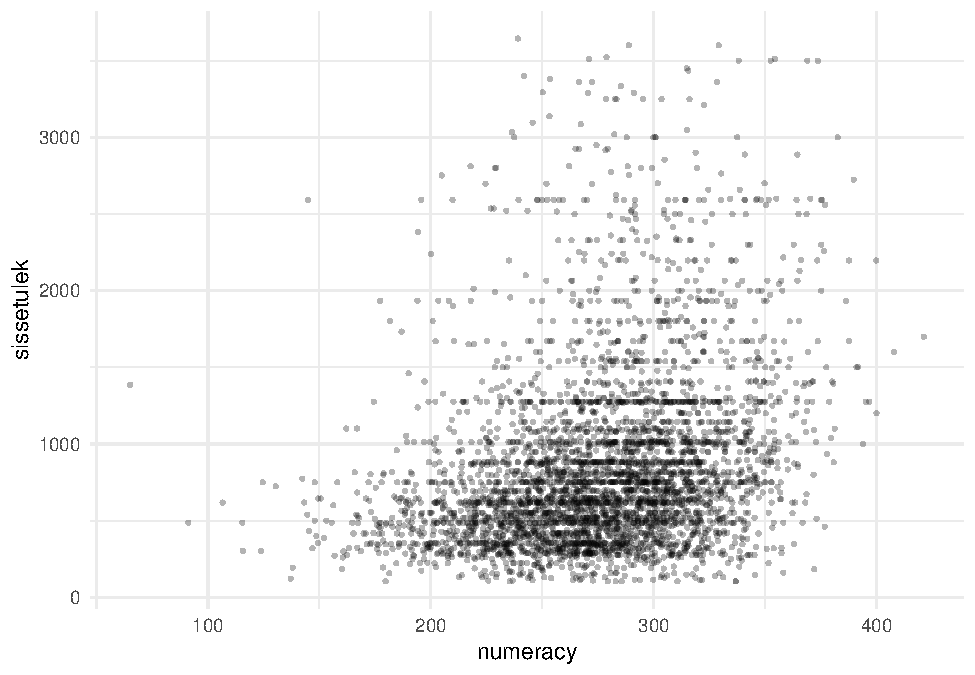
\includegraphics{01-regressioon_files/figure-latex/reg-plot-1-1.pdf}

Tundub, et nende kahe tunnuse vahel on seos olemas. Mida kõrgem on matemaatilise kirjaoskuse skoor, seda kõrgem on sissetulek. Me saame selle suhte kokku võtta regressioonisirge abil. ggplotis on olemas vastav funktsioon \texttt{geom\_smooth()}, mis selle joone meile graafikule paneb. Kuna me tahame saada lineaarse regressiooni sirget, siis peame \texttt{geom\_smooth}'is kasutama argumenti \texttt{method\ =\ "lm"}\footnote{\emph{Defaultis} annab \texttt{geom\_smooth} meile mittelineaarse regressioonijoone (vastavalt sellele palju vaatlusi on, kas \emph{gam} või \emph{loess}), mis üritab tunnustevahelist suhet andmete kõikides punktides võimalikult täpselt kirjeldada.}

\begin{Shaded}
\begin{Highlighting}[]
\NormalTok{piaac }\SpecialCharTok{\%\textgreater{}\%} 
  \FunctionTok{ggplot}\NormalTok{(}\FunctionTok{aes}\NormalTok{(}\AttributeTok{x =}\NormalTok{ numeracy, }\AttributeTok{y =}\NormalTok{ sissetulek))}\SpecialCharTok{+}
  \FunctionTok{geom\_point}\NormalTok{(}\AttributeTok{size =} \FloatTok{0.3}\NormalTok{, }\AttributeTok{alpha =} \FloatTok{0.2}\NormalTok{)}\SpecialCharTok{+}
  \FunctionTok{geom\_smooth}\NormalTok{(}\AttributeTok{method =} \StringTok{"lm"}\NormalTok{, }\AttributeTok{se =}\NormalTok{ F, }\AttributeTok{color =} \StringTok{"\#972D15"}\NormalTok{)}\SpecialCharTok{+}
  \FunctionTok{theme\_minimal}\NormalTok{()}
\end{Highlighting}
\end{Shaded}

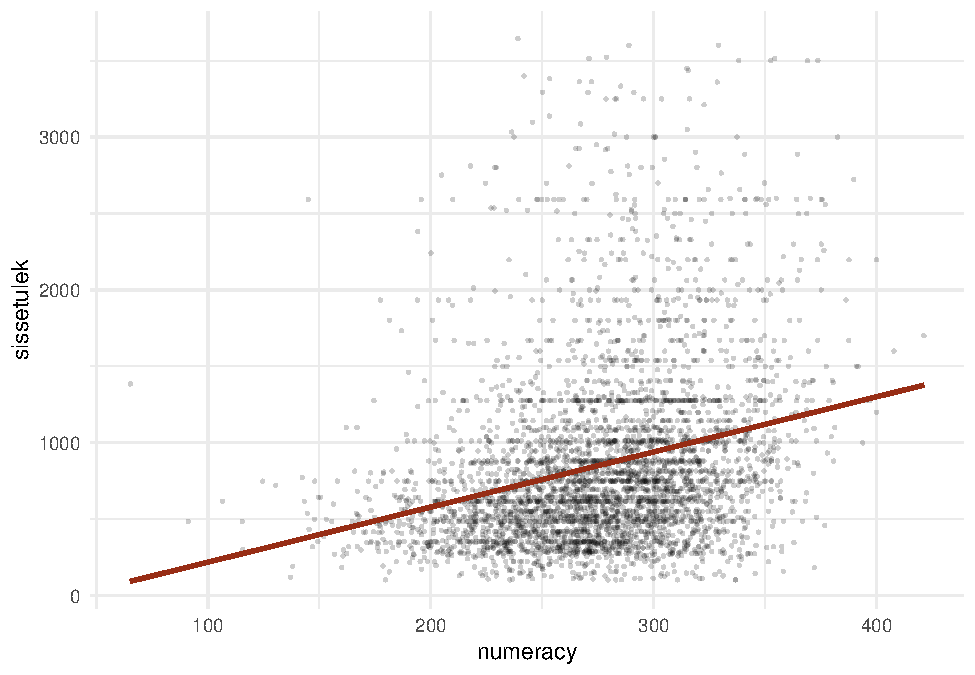
\includegraphics{01-regressioon_files/figure-latex/reg-plot-2-1.pdf}

Regressioonisirge on väljendatav tavalise joone võrrandiga:

\begin{equation}
Y=a+bX
\end{equation}

kus \(a\) on vabaliige (\emph{intercept}) ja \(b\) on sirge tõus (\emph{slope}). Regressiooni kontekstis kutsutakse seda sirge tõusu regressioonikoefitsiendiks või regressioonikordajaks. Vabaliige tähistab \(Y\) väärtust juhul kui \(X\) on \(0\) (sirge lõikumine y-teljega) ja sirge tõus ühikulist muutust \(Y\) väärtuses kui \(X\) väärtus muutub ühe ühiku võrra. Eelneva näite puhul oleks vabaliige võrdne sissetulekuga (\(Y\)) juhul kui matemaatilise kirjaoskuse tase (\(X\)) oleks \(0\) ja sirge tõus võrdne keskmise sissetuleku muutusega, mis lisandub iga matemaatilise kirjaoskuse punktiga. Kui sirge tõus on positiivne, siis \(X\)'i väärtuse kasvades \(Y\) väärtus suureneb, kui negatiivne, siis kahaneb. Kui sirge tõus on aga \(0\), siis seos kahe tunnuse vahel puudub (iga \(X\) väärtuse korral on keskmine \(Y\) sama).

Linaarse regressioonanalüüsi eesmärgiks ongi leida parim võimalik sirge (st leida vabaliige ja regressioonikoefitsient, mis seda sirget määratlevad) tunnustevahelise lineaarse suhte kirjeldamiseks. Parim võimalik tähendab siinjuures seda, et see sirge läheb punktiparvest läbi võimalikult keskelt, st kirjeldab kõiki punkte võimalikult hästi.

\hypertarget{regressioon-r-is}{%
\section{Regressioon R-is}\label{regressioon-r-is}}

R-is käib lihtsa regressioonimudeli tegemine \texttt{lm()} (\emph{linear model}) funktsiooniga. Loomulikult on ka teisi funktsioone, mis regressiooni jooksutamisega hakkama saavad ja hea tahtmise korral võib vastava funktsiooni ka mõningase vaevaga ise valmis kirjutada. Kuid jätame teised variandid hetkel kõrvale.

\texttt{lm()} funktsioonis tuleb defineerida regressioonivõrrand. Selleks peame määratlema sõltuva tunnuse, seejärel kasutama tildet (\texttt{\textasciitilde{}}) ning seejärel määratlema sõltumatu(d) tunnuse(d): \texttt{sõltuv\_tunnus\ \textasciitilde{}\ sõltumatu\_tunnus}\footnote{Hiljem, kui meil on mitu sõltumatut tunnust, eristame tunnused plussiga: \texttt{sõltuv\_tunnus\ \textasciitilde{}\ sõltumatu\_tunnus\_1\ +\ sõltumatu\_tunnus\_2\ +\ ...}}. Võtame eelpool toodud näite sissetuleku ja matemaatilise kirjaoskuse seosest ning defineerime regressioonimudeli, millega hindame matemaatilise kirjaoskuse mõju sissetulekule\footnote{Tegelikult ei ole selline mudel korrektne. Sissetuleku jaotus ei vasta hästi regressiooni nõuetele. Miks ei vasta ja kuidas see vastama panna, sellest natuke hiljem. Kuid hetkel kasutame seda puhtalt didaktilistest kaalutustest lähtuvalt.}:

\begin{Shaded}
\begin{Highlighting}[]
\FunctionTok{lm}\NormalTok{(sissetulek }\SpecialCharTok{\textasciitilde{}}\NormalTok{ numeracy, }\AttributeTok{data =}\NormalTok{ piaac)}
\end{Highlighting}
\end{Shaded}

\begin{verbatim}
## 
## Call:
## lm(formula = sissetulek ~ numeracy, data = piaac)
## 
## Coefficients:
## (Intercept)     numeracy  
##    -140.887        3.606
\end{verbatim}

Lihtsalt \texttt{lm()} funktsiooni jookustades saame kaks numbrit - vabaliikme (\emph{intercept}), mis antud näite puhul on \(-140\), ja regressioonikoefitsiendi (\emph{regression coefficient}), mis antud näite puhul on \(3.6\). Mida need meile ütlevad? Nagu eelnevalt juttu oli, siis vabaliige on \(Y\) väärtus kui \(X\) on \(0\), ehk siis inimesel, kelle matemaatilise kirjaoskuse skoor on \(0\), peaks meie mudeli kohaselt sissetulek olema \(-140\). Regressioonikoefitsient aga annab meile teada kui palju \(Y\) muutub, kui \(X\) muutub ühe ühiku võrra, ehk siis kui matemaatilise kirjaoskuse skoor tõuseb ühe punkti võrra, tõuseb sissetulek keskmiselt \(3.6\) euro võrra.
Nüüd, kui teame mudeli parameetreid, saame nende abil regressioonijoone graafikule kanda ka ilma \texttt{geom\_smooth}'ita:

\begin{Shaded}
\begin{Highlighting}[]
\NormalTok{piaac }\SpecialCharTok{\%\textgreater{}\%} 
  \FunctionTok{ggplot}\NormalTok{(}\FunctionTok{aes}\NormalTok{(}\AttributeTok{x =}\NormalTok{ numeracy, }\AttributeTok{y =}\NormalTok{ sissetulek))}\SpecialCharTok{+}
  \FunctionTok{geom\_point}\NormalTok{(}\AttributeTok{size =} \FloatTok{0.3}\NormalTok{, }\AttributeTok{alpha =} \FloatTok{0.2}\NormalTok{)}\SpecialCharTok{+}
  \FunctionTok{geom\_abline}\NormalTok{(}\AttributeTok{slope =} \FloatTok{3.6}\NormalTok{, }\AttributeTok{intercept =} \SpecialCharTok{{-}}\DecValTok{140}\NormalTok{, }\AttributeTok{color =} \StringTok{"\#972D15"}\NormalTok{)}\SpecialCharTok{+}
  \FunctionTok{coord\_cartesian}\NormalTok{(}\AttributeTok{xlim =} \FunctionTok{c}\NormalTok{(}\DecValTok{0}\NormalTok{,}\DecValTok{450}\NormalTok{), }\AttributeTok{ylim =} \FunctionTok{c}\NormalTok{(}\DecValTok{0}\NormalTok{,}\DecValTok{3500}\NormalTok{))}\SpecialCharTok{+}
  \FunctionTok{theme\_minimal}\NormalTok{()}
\end{Highlighting}
\end{Shaded}

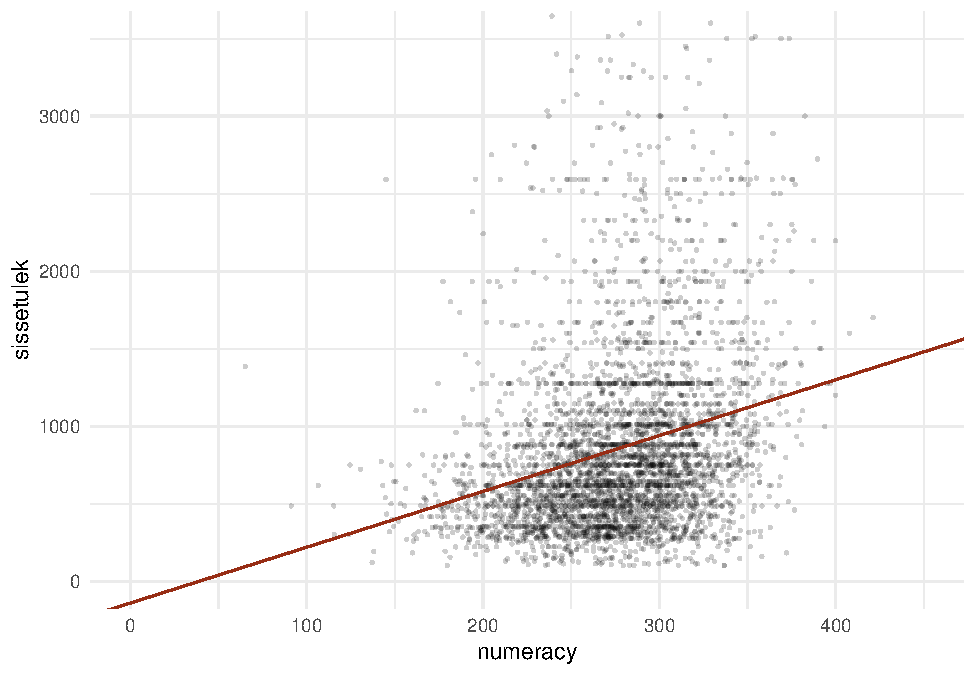
\includegraphics{01-regressioon_files/figure-latex/reg-plot-3-1.pdf}

Kui me teame regressioonisirge tõusu ehk regressioonikoefitsienti ja vabaliiget, siis lähtuvalt sõltumatu tunnuse väärtustest saame prognoosida sõltuva tunnuse väärtuse:

\begin{equation}
\hat{y}_i=b_0+b_1x_i
\end{equation}

\(\hat{y}_i\) antud võrrandis tähistab hinnatud või prognoositud \(y\) väärtust (sellest ka see müts \(y\) peal) vaatlusele \(i\). Kui meil on regressioonivõrrand \(\hat{y}_i=-140+3.6x_i\) ja meil on mingi vaatlus \(i\), kelle \(x\) väärtus on näiteks \(200\), siis saame sellele vaatlusele prognoosida \(y\) väärtuseks \(-140+3.6\times200=580\). Ehk siis inimesel, kelle matemaatilise kirjaoskuse skoor on 200, peaks meie mudeli järgi sissetulek olema \emph{ca} 580 eurot. Inimesel, kelle matemaatilise kirjaoskuse skoor on 400, peaks sissetulek olema keskmiselt \(-140+3.6\times400=1300\) eurot

\begin{figure}
\centering
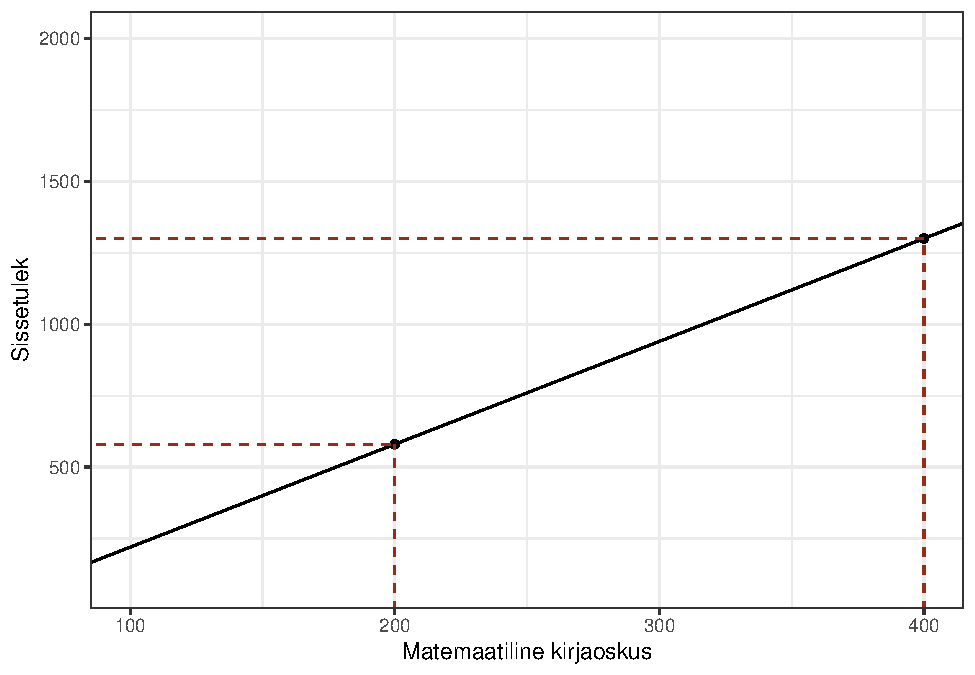
\includegraphics{01-regressioon_files/figure-latex/reg-plot-4-1.pdf}
\caption{\label{fig:reg-plot-4}Prognoosimine y väärtust kui x on 200}
\end{figure}

\hypertarget{regressiooni-juxe4uxe4gid}{%
\section{Regressiooni jäägid}\label{regressiooni-juxe4uxe4gid}}

Samas on muidugi võimatu ühe sirgega kõiki punkte ideaalselt kirjeldada. Iga punkti ja sirge vahele jääb alati mingi viga või teisisõnu, kõik punktid (või vähemalt enamus neist) hälbivad suuremal või vähemal määral regressioonisirgest.

Mida suuremad need hälbed on, seda vähem suudab on meie mudel (regressioonisirge) kirjeldada sõltuva tunnuse variatsiooni ja seda suurem on vea määr meie mudelis. Neid hälbeid kutusutakse \textbf{regressiooni jääkideks} (\emph{regression residuals}).

\begin{figure}
\centering
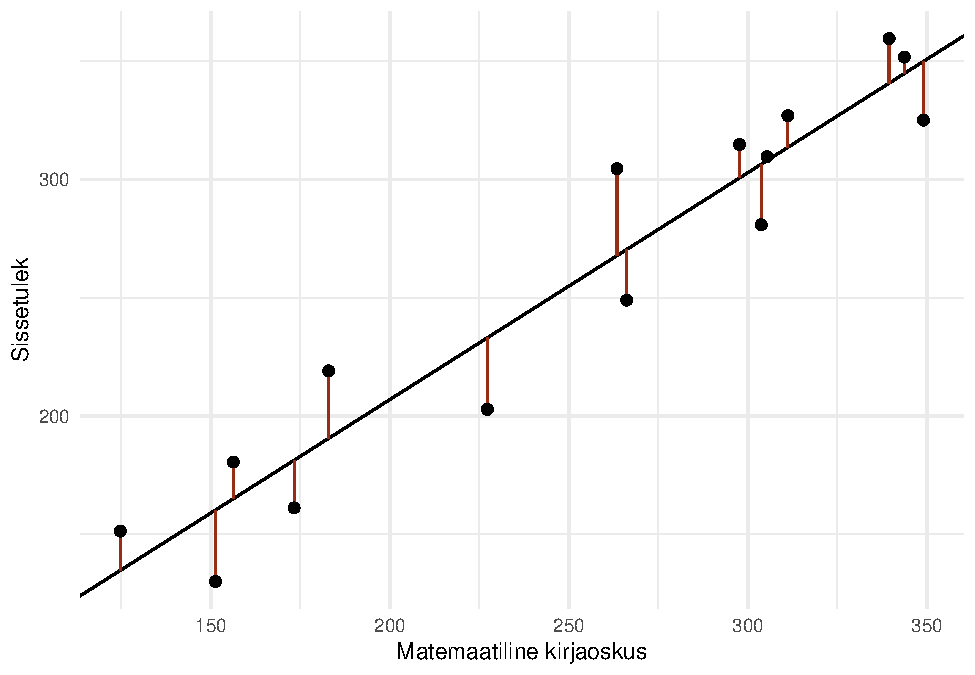
\includegraphics{01-regressioon_files/figure-latex/reg-plot-5-1.pdf}
\caption{\label{fig:reg-plot-5}Regressiooni jäägid}
\end{figure}

Ehk siis iga kord, kui prognoosime \(\hat{y}_i=\beta_0+\beta_1x_i\) abil \(y_i\) väärtust, teeme me mingi vea\footnote{Mida saab väljendada kui \(\epsilon_i=y_i-\hat{y}_i\)}. Seetõttu tuleb regressioonivõrrandile lisada vea komponent (\(\epsilon\)) ning võrrand ise muutub vastavalt:

\begin{equation}
\hat{y_i}=\beta_0+\beta x_i+\epsilon
\end{equation}

Kõige parem regressioonisirge annab joon, mille puhul jäägid on minimaalsed, ehk siis joon, mille puhul kõikide vaatluste jääkide summa oleks võimalikult väike. Kuna me ei saa jääke kokku võtta neid lihtsa kokku liites (\emph{ca} pooled jäägid on väiksemad kui regressioonijoon ja \emph{ca} pooled suuremad, seega nende summa oleks \(0\)), siis tuleb nad enne liitmist ruutu panna. Ja meie eesmärgiks on nüüd leida regressioonisirge, mis minimeeriks \textbf{ruutjääkide summa} (\emph{residual sum of squares} ehk \(RSS\)) ehk siis regressioonisirge, mille puhul \(RSS\) oleks võimalikult väike\footnote{\(RSS= = e_1^2 + e_2^2 + ... + e_n = \sum_{i=1}^{n}(y_i-\hat{y}_i)^2\)}.

Eelnevast lähtuvalt on ka küllaltki loogiline, et meetodit, millega \(RSS\) minimeeritakse ja regressioonisirge ning vastavad koefitsiendid leitakse, nimetatakse \textbf{vähimruutude meetodiks}.

\begin{itemize}
\tightlist
\item
  Kasutades ggplot'i ja tehke punktdiagramm \texttt{geom\_point()} matemaatilise kirjaoskuse (\emph{numeracy}) ja funktsionaalse lugemisoskuse (\emph{literacy}) vahelisest seosest. Pange \emph{numeracy} x-teljele ja \emph{literacy} y-teljele.\\
\item
  Kasutades \texttt{geom\_abline()}'i, lisage joonisele lineaarne regressioonijoon (seega peate eelnevalt \texttt{lm()} funktsiooniga leidma regressioonijoone vabaliikme ja regressioonikoefitsiendi)
\end{itemize}

\color{black}

\hypertarget{regressioonimudeli-sobitumine}{%
\section{Regressioonimudeli sobitumine}\label{regressioonimudeli-sobitumine}}

Olles leidnud joone, mis kirjeldab kahe tunnuse vahelist seost kõige paremini, võiks ju eeldada, et ülesanne on täidetud. Aga kas ikka on? Ükskõik, millisest punktiparvest võib regressioonijoone läbi panna. Kuid tulenevalt regressioonijääkide (vaatluste hälbed regressioonijoonest) suurusest saame selle joone kohta teha väga erinevaid järeldusi. Kui jäägid on väikesed, siis võime suhteliselt täpselt prognoosida sõltuva tunnuse väärtust või teha järeldusi seose kohta. Kuid mida suuremad on jäägid, seda ebatäpsem on ka meie prognoos/järeldus.

Üldjuhul kasutame regresioonanalüüsi, et teha valimi baasil järeldusi mingi üldkogumi kohta. Meid huvitab, kas see seos, mida näeme oma valimi andmete põhjal, kehtib ka üldkogumis. Saame küll eeldada, et valimipõhiselt leitud regressioonisirge on suhteliselt sarnane üldkogumi sirgele (sirge, mille me saaksime, kui kaasaksime analüüsi kõik üldkogumi liikmed), aga kui sarnane, seda me ei tea. Kui me võtaksime samast üldkogumist teise valimi, siis juhul, kui mõlemad valimid on võetud korrektselt\footnote{Korrektse valimi võtmise all peame siinkohal silmas eelkõige juhuvalikut. Kõikidel populatsiooni liikmetel/elementidel peab olema võrdne võimalus valimisse sattuda. Kui üldpopulatsiooniks on Eesti elanikkond, aga valimisse võtaksime ainult Tallinna elanikud, siis antud valimi põhjal tehtavad järeldused ei oleks kuidagi üldistatavad kõigile Eesti elanikele, vaid ikkagi ainult tallinnlastele. Lisaks juhuvalimile on veel terve rida spetsiifilisemaid valimidisaine (stratifitseeritud valim, klastervalim jne) mida me hetkel ei käsitle. Kuid tuleb meeles pidada, et keerulisemate valimidisainide puhul tuleb hilisemas analüüsis ja järelduste tegemise käigus valimi moodustamise loogikat arvesse võtta.} ja valimid on piisavalt suured, siis peaksid nende põhjal leitud regressioonisirged olema suhteliselt sarnased, aga identsed ei ole nad praktiliselt kunagi. Kõikide võimalike valimite puhul me mingil määral alahindame või ülehindame tegelikku, populatsiooni regressioonikoefitsienti (ja ka vabaliiget). Seega, et saada aimu valimipõhise hinnangu täpsusest (vastavusest tegelikule tegelikule üldkogumi parameetrile), peaksime kuidagi välja selgitama valimi kasutamisest tuleneva vea võimaliku suuruse.

Et hinnata mudeli sobivust andmetega ja sellega leitud hinnagute täpsust, vajame mudeli kohta täiendavat infot. Eelnevalt regressioonimudelit \texttt{lm()} funktsiooniga jooksutades oli väljund väga lakooniline. Saime teada ainult vabaliikme ja regressioonikoefitsinedi väärtused. Tegelikult on \texttt{lm()} tulem muidugi märksa põhjalikum. Muule mudeliga kaasnevale infole saame ligi kui salvestame mudeli esmalt mingisse andmeobjekti ja kasutame selle andmeobjekti peal \texttt{summary()} käsku\footnote{Ka \texttt{summary()} ei anna välja kogu mudeliobjektis sisalduvat infot. Et näha mida mudeliobjekt veel sisaldab, võib kasutada \texttt{str(mudeliobjekt)} käsku.}.

\begin{Shaded}
\begin{Highlighting}[]
\NormalTok{mudel1 }\OtherTok{\textless{}{-}} \FunctionTok{lm}\NormalTok{(sissetulek }\SpecialCharTok{\textasciitilde{}}\NormalTok{ numeracy, }\AttributeTok{data =}\NormalTok{ piaac)}
\FunctionTok{summary}\NormalTok{(mudel1)}
\end{Highlighting}
\end{Shaded}

\begin{verbatim}
## 
## Call:
## lm(formula = sissetulek ~ numeracy, data = piaac)
## 
## Residuals:
##     Min      1Q  Median      3Q     Max 
## -1016.7  -351.5  -129.1   179.4  2923.4 
## 
## Coefficients:
##             Estimate Std. Error t value Pr(>|t|)    
## (Intercept) -140.887     56.510  -2.493   0.0127 *  
## numeracy       3.606      0.202  17.849   <2e-16 ***
## ---
## Signif. codes:  0 '***' 0.001 '**' 0.01 '*' 0.05 '.' 0.1 ' ' 1
## 
## Residual standard error: 555.8 on 3982 degrees of freedom
##   (3648 observations deleted due to missingness)
## Multiple R-squared:  0.07408,    Adjusted R-squared:  0.07385 
## F-statistic: 318.6 on 1 and 3982 DF,  p-value: < 2.2e-16
\end{verbatim}

\begin{Shaded}
\begin{Highlighting}[]
\CommentTok{\# Kui me ei taha mudelit salvestada, siis saab ka nii:}
\FunctionTok{summary}\NormalTok{(}\FunctionTok{lm}\NormalTok{(numeracy }\SpecialCharTok{\textasciitilde{}}\NormalTok{ literacy, }\AttributeTok{data =}\NormalTok{ piaac))}
\end{Highlighting}
\end{Shaded}

Nüüd näeme juba märksa põhjalikumat väljundit. Vaatame mis seal kirjas on ja kuidas seda tõlgendada. Käime väljundi sektsioonide kaupa läbi (v.a. esimene rida, mis on vist niigi suht selge)

\hypertarget{juxe4uxe4kide-jaotus}{%
\subsection{Jääkide jaotus}\label{juxe4uxe4kide-jaotus}}

\begin{verbatim}
## Residuals:
##     Min      1Q  Median      3Q     Max 
## -1016.7  -351.5  -129.1   179.4  2923.4
\end{verbatim}

Väljundis on kirjeldatud regressiooni jääkide (\emph{residuals}) jaotus. Enne nägime, et regressiooni jäägid on regressioonijoone ja tegelike, vaadeldud väärtuste vahe. Mida väiksemad on jäägid, seda täpsemini kirjeldab regressioonijoon andmete vahelist seost. Nägime ka, et pooled jäägid peaksid ideaalis olema suuremad (positiivse märgiga) kui regressioonisirge ja pooled väiksemad (negatiivse märgiga). Seega peaks jääkide keskmine olema ligikaudu \(0\) ning jääkide jaotus normaaljaotuse sarnane, kus esimene ja kolmas kvartiil, aga ka maksimum ja miinimum, on keskväärtusest umbes sama kaugel. Hiljem vaatame jääkide jaotust ka graafiliselt, mis on märksa mõistlikum viis neid uurida, kuid esmase mulje saab ka siit kätte.

\hypertarget{regressioonikoefitsiendid-ja-nende-olulisus}{%
\subsection{Regressioonikoefitsiendid ja nende olulisus}\label{regressioonikoefitsiendid-ja-nende-olulisus}}

\begin{verbatim}
##             Estimate Std. Error t value Pr(>|t|)    
## (Intercept) -140.887     56.510  -2.493   0.0127 *  
## numeracy       3.606      0.202  17.849   <2e-16 ***
## ---
## Signif. codes:  0 '***' 0.001 '**' 0.01 '*' 0.05 '.' 0.1 ' ' 1
\end{verbatim}

Koefitsientide sektsioonis on esitatud mudeli oluliseim info. \textbf{\emph{Estimate}} on hinnang mudeliga leitud regressioonikoefitsientidele. Lihtsa regressiooni puhul on meil ainult vabaliige ja ühe sõltumatu tunnuse koefitsient. Hiljem, mitmese regressiooni kontekstis, on neid koefitsiente rohkem. Vabaliikmeid on aga mudeli kohta alati üks.

Tulbas \textbf{\emph{Std. Error}} on toodud koefitsientide standardvead. Standardviga kirjeldab meie mudeli hinnangus sisalduvat määramatust. Me kasutame regressioonikoefitsientide leidmiseks üldjuhul valimipõhiseid andmeid, kuigi tegelikult huvitavad meid ju üldkogums esinevad seosed. Valimipõhine hinnang peaks piisavalt suure valimi korral olema tõenäoliselt küllaltki sarnane üldkogumi vastavale parameetrile, kuid väikese valimi korral puhta juhuse läbi sellest arvestatavalt erineda. Standardviga näitabki kui kindlad me oma mudeli hinnangus olla saame. Mida väiksem on standardviga (võrreldes hinnangu endaga), seda kindlamad võime olla ka oma hinnangus. Standardvea suurs sõltub eelkõige jääkide hajuvusest ja valimi suurusest. Mida väiksemad on jäägid ja mida suurem on valim, seda väiksem on ka standardviga.

Standardvea abil saame \emph{t}-testi abil testida, kas regressioonikoefitsient erineb oluliselt nullist (kui koefitsient on null, siis seos tunnuste vahel puudub). \emph{t}-testi tulemust näitab veerg \textbf{\emph{t value}}. \emph{t}-väärtus ütleb meile kui mitme standardvea kaugusel meie regressioonikoefitsient 0-st on. Kui on piisavalt kaugel, siis saame järeldada, et leitud koefitsient on ka üldkogumis 0-st erinev. Kui kaugel on aga piisavalt kaugel? See sõltub sellest, kui suurt vea tõenäosust me oleme valmis tolereerima (mingi vea tõenäosus jääb seejuures alati). Üldjuhul valitakse selleks tõenäosuseks \(5\%\) (ütleme, et regressioonikoefitsient on statistiliselt oluline usaldusnivool \(95 \%\) või olulisusnivool \(p < 0.05\)), aga see võib olla ka \(1\%\) või \(10\%\). Siin tegelikult ei ole mingit väga konkreetset piirmäära, millest juhinduda. Kui me aga lepime kokku, et võimaliku vea tõenäosusena aktsepteerime \(5\)-te protsenti, siis peab \emph{t}-väärtus olema suurem kui \emph{ca} \(\pm2\) (täpne väärtus sõltub vaatluste arvust). Antud näite puhul on \emph{t}-väärtused \(-2.5\) ja \(17.8\), ehk siis mõnevõrra suuremad kui \(\pm2\) ja me võime järeldada, et nii vabaliige kui regressioonikoefitsient erinevad olulisusnivool \(95\%\) oluliselt nullist (kuigi jah, vabaliige on suhteliselt piiri peal).

Õnneks ei pea me seda täpset \emph{t}-väärtuse piirmäära ise välja nuputama. R arvutab meile automaatselt võimaliku vea tõenäosuse konkreetse \emph{t}-väärtuse kohta. See tõenäosus on ära toodud veerus \textbf{\emph{Pr(\textgreater\textbar t\textbar)}} ja seda nimetatakse \emph{p}-väärtuseks. \emph{p}-väärtuse tõlgendus on: kui tõenäoline on, et me saaksime niivõrd suure või suurema \emph{t}-väärtuse nagu me saime, kui regressioonikoefitsient oleks üldkogumis tegelikult \(0\). Seega kui \emph{p}-väärtus on näiteks \(0.04\), siis oleks tõenäosus, et me saaksime sellise regressioonikoefitsiendi, juhul kui üldkogumis oleks regressioonikoefitsient tegelikult \(0\) (ehk tunnuste vahe seost ei oleks), \(0.04\) ehk \(4\)\% või väiksem. Üldjuhul tahaksime näha \emph{p}-väärtust, mis on väiksem kui \(0.05\). Sellisel juhul oleks koefitsient statistiliselt oluline usaldusnivool \(95\%\). Antud näites on meil regressioonikoefitsiendi puhul tegemist väga väikeste \emph{p} väärtustega (\textless2e-16 tähendab väiksem kui \(2\times10^{-16}\)) ja me võime olla päris kindlad, et koefitsient erineb nullist. Vabaliikme \emph{p}-väärtus on aga \(0.012\), ehk kui me kasutaksime usaldusnivood \(99\%\) (mille puhul \emph{p}-väärtus peaks olema väiksem kui \(0.01\)), siis me ei saaks järeldada, et see on statistiliselt oluliselt erinev nullist. Lisaks kuvab R iga \emph{p}-väärtuse taha ka tärnid, mis indikeerivad selle väärtuse suurust lähtuvalt allolevast legendist.

Miks meil on üldse vaja teada kas koefitsiendid erinevad oluliselt nullist? Aga sellepärast, et kui regressioonisirge oleks \(0\), siis meie tunnuste vahel ei oleks seost (kui \(X\) muutub \(1\) ühiku võrra, siis \(Y\) muutub \(0\) ühiku võrra, ehk siis \(Y\) väärtus ei sõltu \(X\)'i väärtusest). Aga kuidas on lood vabaliikmega? Kas ka see peab erinema nullist, et meie mudelist mingit tolku oleks? Tegelikult ju ei pea. Võib täitsa vabalt juhtuda, et regressioonisirge lähebki läbi \(X\) ja \(Y\) telgede ristumiskoha (\(Y\) on \(0\) kui \(X\) on \(0\)). Sellisel juhul oleks vabaliikme \emph{t}-väärtus väiksem kui \(2\) ja \emph{p}-väärtus suurem kui 0.05, kuid mudeli tõlgendust see ei mõjutaks. Ehk siis tavaliselt meid vabaliikme \emph{p} ja \emph{t} väärtused väga ei huvita. Küll aga peaks jälgima, et standardviga väga suur (võrreldes vabaliikme endaga) ei oleks.

\hypertarget{juxe4uxe4kide-standardviga}{%
\subsection{Jääkide standardviga}\label{juxe4uxe4kide-standardviga}}

\begin{verbatim}
## Residual standard error: 555.8 on 3982 degrees of freedom
##   (3648 observations deleted due to missingness)
\end{verbatim}

Kuidas hinnata regressiooniprognoosi täpsust, ehk siis seda kui hästi regressioonimudel sobitub andmetega (\emph{model fit})? Üheks võimaluseks on lähtuda samast loogikast mida kasutame tunnuse keskväärtuse täpsuse hindamisel. Ehk kui palju vaatlused keskmiselt erinevad keskväärtusest. Regressioonijoone puhul ei ole meil ühte keskväärtust, mille suhtes vaatluste hälbimist määrata. Kuid iga vaatluse sõltumatu tunnuse väärtuse \(x\) kohta on meil ``hinnatud'' sõltuva tunnuse väärtus \(\hat{y}\). Seega tuleb meil lihtsalt vaadata kui palju vaatluste \(y\) ja \(\hat{y}\) väärtused keskmiselt erinevad, ehk kui suur on keskmine viga meie mudelis. Regressioonanalüüsi kontekstis kutsutakse seda vaatluste varieeruvuse näitajat keskmiseks ruutveaks (\emph{mean squared error}) ehk lühidalt \(MSE\)\footnote{\(MSE=\frac{\sum_{i=1}^{n}(y_i-\hat{y}_i)^2}{n-2}\)}. Kuna aga \(MSE\) väärtus on ruudus, siis on seda keeruline interpreteerida (samamoodi nagu ka dispersiooni). Kui me võtame ruutjuure \(MSE\)'st, \(\sqrt{MSE}\), saame regressiooni jääkide standardhälbe, mida nimetatakse \textbf{jääkide standardveaks} (\emph{residual standard error} ehk RSE). Mida väiksem on mudeli RSE, seda paremini mudel andmetega sobitub (seda vähem hälbivad vaatlused regressioonijoonest ehk seda väiksemad on regresiooni jäägid). See, kui väike peaks RSE väärtus hea mudeli korral olema, sõltub eelkõige kontekstist ja sõltuva tunnuse skaalast (samamoodi nagu keskväärtuse standardhälve). Mingeid konkreetseid piirväärtusi siinkohal tuua ei ole võimalik.\\
Lisaks on siin ära toodud ka \emph{degrees of freedom} ehk vabadusastmete arv jääkide standardvea arvutamisel. Sisuliselt on siin kirjas analüüsi kaasatud vaatluste arv (miinus regressioonikordajate arv, siinses mudelis 2). Ära on toodud ka analüüsist välja jäetud vaatluste arv. Need on need, kellel puudus väärtus vähemalt ühe analüüsitava tunnuse jaoks.

\hypertarget{r-ruut}{%
\subsection{R ruut}\label{r-ruut}}

\begin{verbatim}
## Multiple R-squared:  0.07408,    Adjusted R-squared:  0.07385
\end{verbatim}

Vast oluliseimaks mudeli headuse näitajaks on \(R^2\). Regressioonanalüüsi eesmärk on seletada mingit osa sõltuva tunnuse variatiivsusest sõltumatu tunnuse abil. Seega saame regressioonimudeli puhul hinnata ja mudeli kvaliteedi iseloomustusena kasutada sõltumatu tunnuse poolt seletatud variatiivsuse osakaalu sõltuva tunnuse koguvariatiivsusest. Sõltuva tunnuse variatiivsuse (seda nimetatakse \(TSS\) ehk \emph{total sums of squares}) saab jagada komponentideks: variatiivsus, mis on seletatud regressioonijoone poolt (\(ESS\) ehk \emph{explained sums of squares}) ja variatiivsus, mis ei ole regressioonijoone poolt seletatud ehk siis mudeli seisukohast viga (\(RSS\) ehk \emph{residual sums of squares}):

\[TSS=RSS+ESS\]

\marginnote{

\begin{equation}
ESS=\sum_{i=1}^{n}(\hat{y}_i-\bar{y})^2
\end{equation}

\begin{equation}
RSS=\sum_{i=1}^{n}(y_i-\hat{y}_i)^2
\end{equation}

\begin{equation}
TSS=\sum_{i=1}^{n}(y_i-\bar{y})^2
\end{equation}

}

Teades erinevaid variatiivsuse komponente, saame määrata kui suur osa (mitu protsenti) sõltuva tunnuse koguvariatsioonist on seletatav regressioonijoone poolt (ehk siis sõltumatu tunnuse poolt). Seda suurust nimetatakse \textbf{determinatsioonikordajaks} ehk lühidalt \(R^2\)-ks.

\begin{equation}
R^2=\frac{TSS-RSS}{TSS}=1-\frac{RSS}{TSS}
\end{equation}

\begin{figure}
\centering
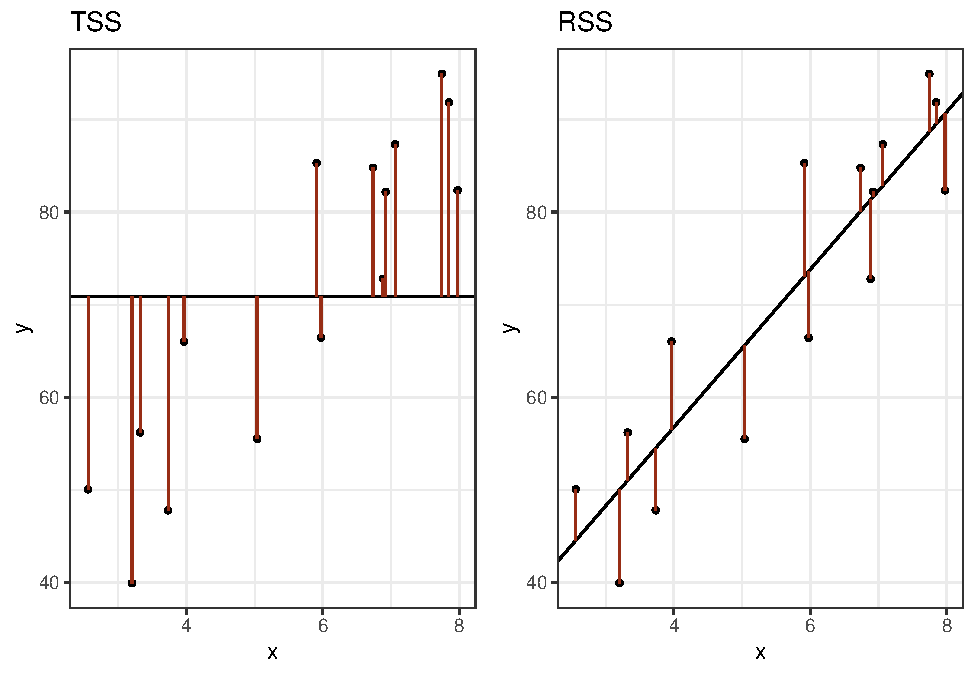
\includegraphics{01-regressioon_files/figure-latex/ss-1.pdf}
\caption{\label{fig:ss}Variatsiivsuse jagunemine}
\end{figure}

\(R^2\) jääb vahemikku \(0-1\). See mõõdab seose tugevust, st mida lähemal \(R^2\) on \(1\)'le, seda tugevam lineaarne seos tunnuste vahel on ja seda enam sõltumatu tunnus sõltuva tunnuse variatsiooni seletab, seega seda efektiivsem on regressioonifunktsiooni kasutamine selle asemel, et lihtsalt sõltuva tunnuse keskmist hinnata (kui \(R^2\) on \(0\), siis regressioonijoon langeb kokku sõltuva tunnuse keskmist tähistava joonega, st et \(ESS=0\) ja \(TSS=RSS\)).

R annab meile lisaks tavalisele \(R^2\) väärtusele (\emph{Multiple R-squared}) ka nn korrigeeritud \(R^2\) väärtuse (\emph{Adjusted R-squared}). Korrigeeritud \(R^2\) puhul võetakse arvesse ka sõltumatute tunnuste arvu. Iga lisanduva sõltumatu tunnusega läheb ``tavaline'' \(R^2\) suuremaks. Kui lisanduv tunnus eriti midagi ei seleta, siis võib see tõus olla väga väike, kuid mingi tõus paratamatult on. Korrigeeritud \(R^2\), arvestades oma valemis ka sõltumatute tunnuste arvu, annab mitme sõltumatu tunnuse korral korrektsema tulemuse. Hetkel, lihtsa regressiooni kontekstis, kus meil on ainult üks sõltumatu tunnus, annavad mõlemad variandid (enam-vähem) sama tulemuse.

\hypertarget{f-vuxe4uxe4rtus-ja-f-test}{%
\subsection{F-väärtus ja F-test}\label{f-vuxe4uxe4rtus-ja-f-test}}

\begin{verbatim}
## F-statistic: 318.6 on 1 and 3982 DF,  p-value: < 2.2e-16
\end{verbatim}

\emph{F}-väärtus, sarnaselt \emph{t}-väärtusele, aitab meil hinnata kas meie mudel on statistiliselt oluline, ehk siis kas meie analüüsitavate tunnuste vahel on oluline lineaarne seos. \emph{F}-väärtuseks nimetatakse mudeli abil seletatud variatiivsuse ja seletamata variatiivsuse suhet\footnote{Natuke täpsemalt väljendades \(F = \frac{(TSS-RSS)/p}{RSS/(n-p-1)}\), kus \(n\) on valimi suurus ja \(p\) on regressioonikoefitsientide (sõltumatute muutujate) arv.}:

\begin{equation}
\text{F-suhe} = \frac{\text{regressioonimudeli poolt seletatud variatiivsus}}{\text{regressioonimudeli poolt seletamata variatiivus}}
\end{equation}

Kui mudeli regressioonisirge on \(0\), siis peaks see suhe olema \(1\). See tähendab, et regressioonisirge ei seleta üldse sõltuva tunnuse varieeruvust. Kui regressioonisirge on suurem kui \(0\) siis peaks regressioonisirge poolt seletatud varieeruvus (koos juhusliku varieeruvusega) olema suurem kui ainult juhuslik dispersioon. Saame jällegi kasutada \emph{F}-väärtusega kaasnevat \emph{p} väärtust, et hinnata kas see \emph{F}-väärtus on piisavalt suur, et saaksime mudelist lähtuvalt mingeid sisukaid järeldusi teha.

Võite märgata, et need kaks testi regressioonimudeli kohta annavad sama \emph{p} väärtuse. Ja tegelikult annavad nad ka sama teststatistiku. \emph{t}-statistik on lihtsalt ruutjuur \emph{F} statistikust\footnote{\((t^{*}_{(n-2)})^2=F^{*}_{(1,n-2)}\)}. Võib tekkida küsimus, et miks me siis kahte testi peame kasutama. Ühe sõltumatu tunnusega regressioonimudelis otseselt ei peagi. Samas kui meil on mitu sõltumatut tunnust (nagu meil hiljem on), siis \emph{F} ja \emph{t} väärtused muutuvad. \emph{F}-testiga saab sel juhul testida terve mudeli headust, st kas meie sõltumatud tunnused koos suudavad seletada piisavalt sõltuva tunnuse variatiivsust (tegelikult testib \emph{F}-test seda, et kas vähemalt üks koefitsientidest erineb nullist). \emph{t}-statistikud aga arvutatakse igale regressioonikoefitsiendile eraldi ning nendega saame kontrollida iga üksiku koefitsiendi erinevust nullist.

\begin{itemize}
\tightlist
\item
  Looge regressioonimudel, millega hindate \emph{numeracy} mõju \emph{literacy}'le.\\
\item
  Salvestage see mudel ja uurige \texttt{summary()} funktsiooniga.
\item
  Kas \emph{numeracy} mõju \emph{literacy}'le on statistiliselt oluline?\\
\item
  Mitu protsenti \emph{literacy} variatsioonist on selgitatav läbi \emph{numeracy}?
\end{itemize}

\hypertarget{kategoriaalsed-tunnused-regressioonis}{%
\section{Kategoriaalsed tunnused regressioonis}\label{kategoriaalsed-tunnused-regressioonis}}

\hypertarget{uxfcks-binaarne-suxf5ltumatu-tunnus}{%
\subsection{Üks binaarne sõltumatu tunnus}\label{uxfcks-binaarne-suxf5ltumatu-tunnus}}

Siiani oleme käsitlenud ainult mudeleid, kus sõltumatuteks tunnusteks on pidevad muutujad. Kuid me saame mudelisse lülitada ka kategoriaalseid tunnuseid. Vaatame esmalt mudelit, kus on üks kategoriaalne sõltumatu muutuja\footnote{Sellist mudelit nimetatakse ka ANOVA-ks või täpsemlat One-Way ANOVA-ks (kuna tegemist on ainult ühe kategoriaalse sõltumatu muutujaga)}. Teeme Piaaci andmete põhjal mudeli, millega hindame soo mõju sissetulekule

\begin{Shaded}
\begin{Highlighting}[]
\NormalTok{mudel2 }\OtherTok{\textless{}{-}} \FunctionTok{lm}\NormalTok{(sissetulek }\SpecialCharTok{\textasciitilde{}}\NormalTok{ sugu, }\AttributeTok{data =}\NormalTok{ piaac)}
\FunctionTok{summary}\NormalTok{(mudel2)}
\end{Highlighting}
\end{Shaded}

\begin{verbatim}
## 
## Call:
## lm(formula = sissetulek ~ sugu, data = piaac)
## 
## Residuals:
##    Min     1Q Median     3Q    Max 
## -974.0 -344.0 -122.7  198.1 2755.2 
## 
## Coefficients:
##             Estimate Std. Error t value Pr(>|t|)    
## (Intercept)  1077.90      13.35   80.73   <2e-16 ***
## suguNaine    -383.15      17.52  -21.86   <2e-16 ***
## ---
## Signif. codes:  0 '***' 0.001 '**' 0.01 '*' 0.05 '.' 0.1 ' ' 1
## 
## Residual standard error: 545.8 on 3982 degrees of freedom
##   (3648 observations deleted due to missingness)
## Multiple R-squared:  0.1072, Adjusted R-squared:  0.107 
## F-statistic:   478 on 1 and 3982 DF,  p-value: < 2.2e-16
\end{verbatim}

Kuidas seda tulemust tõlgendada?

Regressioonimudeliga hindame \(\hat{y_i}\) väärtust vaatlusele \(i\), kui sõltumatu tunnuse väärtus muutub ühe ühiku võrra. \(\hat{y_i}\)'i väärtus kujuneb siis lähtuvalt vabaliikme \(\beta_0\) ja regressioonikoefitsiendi \(\beta\) ning sõltumatu tunnuse \(x_i\)'i korrutise summast (pluss mingi viga): \(\hat{y_i}=\beta_0+\beta x_i+\epsilon\). Sealjuures vabaliige on \(y\) väärtus kui \(x\) on \(0\).

Meil on tunnus \(x\) (sugu) kahe kategooriaga. Mis juhtub, kui kodeerime selle ümber väärtusteks \(0\) ja \(1\) (vastavalt mees ja naine). R kusjuures teeb seda automaatselt.

\[ x_{i} =
  \begin{cases}
    1  & \quad \text{kui on naine}\\
    0  & \quad \text{kui on mees}
  \end{cases}
\]

Kui me selle tunnuse nüüd regressioonivõrrandisse paneme, siis mis on \(y_i\) väärtus kui \(x_i\) on \(1\) (ehk siis vaatluse sugu on naine) ja mis on \(y_i\) väärtus kui \(x_i\) on \(0\) (ehk siis vaatluse sugu on mees)?

\[ \hat{y_i}=\beta_0+\beta_1 x_i+\epsilon =
  \begin{cases}
    \beta_0+\beta_1 \times 1 = \beta_0+\beta_1  & \quad \text{kui on naine}\\
    \beta_0+\beta_1 \times 0 = \beta_0  & \quad \text{kui on mees}
  \end{cases}
\]

Ehk siis kui \(x_i\) väärtus on \(0\) (mehed), siis võrdub \(\hat{y_i}\) vabaliikmega \(\beta_0\) (sest \(\beta_1\) korrutatakse läbi nulliga) ja kui \(x_i\) väärtus on \(1\) (naised), siis vabaliikme ja regressioonikoefitsiendi summaga \(\beta_0+\beta\). Mida \(\hat{y}\) antud juhul üldse tähistab? Pidevmuutujaga regressioonis tähistas see keskmist \(y\)-i väärtust erinevate \(x\) väärtuste korral. Ja siin täpselt samamoodi. Aga nüüd on meil ainult kaks \(x\) väärtust ja \(\hat{y}\) on vastavate gruppide (meeste ja naiste) keskmine \(y\).

Seega saame regressioonivõrrandiga väljenda binaarse tunnuse mõju sõltuva tunnuse keskmisele. Lihtsalt käsitleme ühte kategooriat nn \textbf{referentskategooriana} ja kodeerime selle \(0\)'ks. Kui \(x\) on \(0\), siis \(y\) väärtus on võrdne vabaliikme väärtusega. Ja kui sõltumatu tunnuse väärtus muutub ühe ühiku võrra (ja rohkem ta ei saagi muutuda), siis on \(y\) väärtus võrdne vabaliikme väärtus pluss regressioonikoefitsiendi väärtus.

Kuidas me eelneva valguses oma näidet siis tõlgendama peaksime?

\begin{verbatim}
## Coefficients:
##             Estimate Std. Error t value Pr(>|t|)    
## (Intercept)  1077.90      13.35   80.73   <2e-16 ***
## suguNaine    -383.15      17.52  -21.86   <2e-16 ***
\end{verbatim}

\emph{Sugu} oli tekstiline tunnus. R saab aru, et tegemist on kategoriaalse tunnusega ja kodeerib selle sisemiselt ümber \(0\)-ks ja \(1\)-ks. Antud juhul määras ta kategooria \emph{Naine} \(1\)-ks ja kategooria \emph{Mees} \(0\)-ks. Kuna tegemist oli tekstilise tunnusega, siis lähtub R siin tähestikulisest järjekorrast. Regressioonivõrrand oli järgmine:

\begin{equation}
\hat{y_i}=\beta_0+\beta x_i+\epsilon
\end{equation}

Paneme mudeli tulemused sellesse võrrandisse:

\[ \text{numeracy}=1077.90+(-383.15)\times \text{naine} =
  \begin{cases}
    1077.90-383.15\times 1 = 1077.90-383.15 = 694.75  & \quad \text{kui on naine}\\
    1077.90-383.15\times 0 = 1077.90  & \quad \text{kui on mees}
  \end{cases}
\]

Ehk siis naiste keskmine sissetulek on \(694.8\) eurot (vabaliige + regressioonikoefitsient) ja meeste oma \(1077.9\) eurot (vabaliige). Erinevus on statistiliselt oluline, kuna \emph{p}-väärtused nii koefitsiendi \emph{t}-testi kui ka mudeli \emph{F}-testi puhul olid olulisusnivool \(95\%\) olulised (väiksemad kui \(0.05\)).

Kui me paneme need keskmised joonisele ja ühendame nad joonega, näeme, et selle joone tõus (\emph{slope}) on võrdne regressioonikoefitsiendiga, täpselt samuti nagu pidevtunnusega regressioonis.

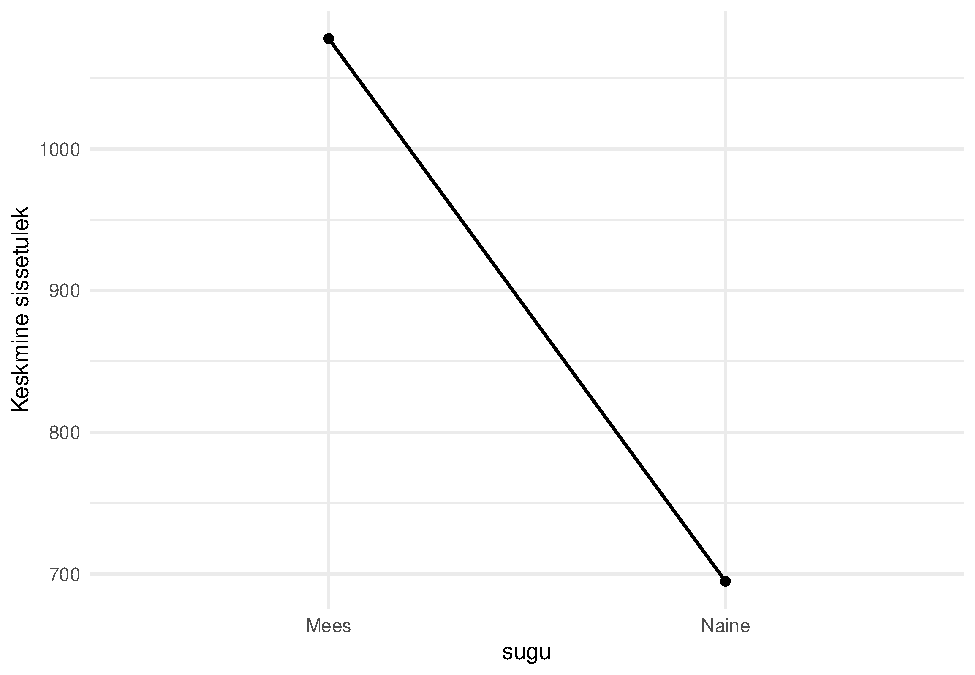
\includegraphics{01-regressioon_files/figure-latex/reg-plot-6-1.pdf}

\hypertarget{kolme-vuxf5i-enama-kategooriaga-suxf5ltumatu-tunnus}{%
\subsection{Kolme või enama kategooriaga sõltumatu tunnus}\label{kolme-vuxf5i-enama-kategooriaga-suxf5ltumatu-tunnus}}

Kusjuures me ei pea piirduma vaid binaarsete tunnustega. Aga kui kategooriaid on rohkem, tuleb meil nad binaarseks teha ehk dihhotomiseerida. Määratleme ühe kategooria referentskategooriana ja ülejäänud kategooriad kodeerime erinevates tunnustes \(1\)'ks. Seega, kui meil on näiteks hariduse tunnus kolme kategooriaga (põhiharidus, keskharidus, kõrgharidus), peame määratlema ühe referentskategooria (näiteks põhiharidus) ja tegema kaks uut tunnust (vastavalt keskhariduse ja kõrghariduse kategooriatele):

\[ kesk_{i} =
  \begin{cases}
    1  & \quad \text{kui inimene on keskharidusega}\\
    0  & \quad \text{kui inimene ei ole keskharidusega}
  \end{cases}
\]

\[ korg_{i} =
  \begin{cases}
    1  & \quad \text{kui inimene on kõrgharidusega}\\
    0  & \quad \text{kui inimene ei ole kõrgaridusega}
  \end{cases}
\]

Nüüd saame iga inimese hariduse määratleda kahe tunnuse kaudu. Ehk siis inimene, kelle puhul \(kesk = 1\) ja \(korg = 0\), on keskharidusega; inimene kelle puhul \(kesk = 0\) ja \(korg = 1\), on kõrgharidusega ja inimene kelle puhul \(keks = 0\) ja \(korg = 0\), on põhiharidusega. \(y\) väärtus kujuneb täpselt samamoodi nagu binaarse tunnuse puhul:

\[y_i=\beta_0+\beta_1 \times kesk_i+\beta_2 \times korg_i+\epsilon_i =\]

\[ =
  \begin{cases}
    \beta_0+\beta_1 \times 1+\beta_2 \times 0 = \beta_0+\beta_1  & \quad \text{kui inimene on keskharidusega}\\
    \beta_0+\beta_1 \times 0+\beta_2 \times 1 = \beta_0+\beta_2  & \quad \text{kui inimene on kõrgaridusega}\\
    \beta_0+\beta_1 \times 0+\beta_2 \times 0 = \beta_0  & \quad \text{kui inimene on põhiharidusega}
  \end{cases}
\]

Vaatame kuidas see kõik R-is välja näeb. Hindame hariduse (tunnus \emph{haridustase}) mõju sissetulekule:

\begin{Shaded}
\begin{Highlighting}[]
\NormalTok{mudel3 }\OtherTok{\textless{}{-}} \FunctionTok{lm}\NormalTok{(sissetulek }\SpecialCharTok{\textasciitilde{}}\NormalTok{ haridustase, }\AttributeTok{data =}\NormalTok{ piaac)}
\FunctionTok{summary}\NormalTok{(mudel3)}
\end{Highlighting}
\end{Shaded}

\begin{verbatim}
## 
## Call:
## lm(formula = sissetulek ~ haridustase, data = piaac)
## 
## Residuals:
##    Min     1Q Median     3Q    Max 
## -868.3 -362.5 -145.2  187.1 2881.2 
## 
## Coefficients:
##                  Estimate Std. Error t value Pr(>|t|)    
## (Intercept)        763.35      13.33  57.279   <2e-16 ***
## haridustaseKõrge   217.23      19.06  11.400   <2e-16 ***
## haridustaseMadal   -22.20      30.17  -0.736    0.462    
## ---
## Signif. codes:  0 '***' 0.001 '**' 0.01 '*' 0.05 '.' 0.1 ' ' 1
## 
## Residual standard error: 567.1 on 3981 degrees of freedom
##   (3648 observations deleted due to missingness)
## Multiple R-squared:  0.03631,    Adjusted R-squared:  0.03583 
## F-statistic:    75 on 2 and 3981 DF,  p-value: < 2.2e-16
\end{verbatim}

R sai jällegi ise aru, et \emph{haridustase} on tekstiline tunnus ja dihotomiseeris selle automaatselt ära, tehes kaks uut tunnust: \emph{haridustaseKõrge} (kus kõik kõrgharitud on kodeeritud \(1\)-na ja kõik teised \(0\)-na) ja \emph{haridustaseMadal} (kus kõik madala haridustasemega on kodeeritud \(1\)-na ja kõik teised \(0\)-na). Referentskategooriaks võttis ta tähestiku järjekorras esimese kategooria \emph{Keskmine} (kõik vaatlused, mille puhul nii \emph{haridustaseKõrge} kui ka \emph{haridustaseMadal} on \(0\)-d, on keskmise haridustasemega).

Tulemuste interpreteerimine toimub samamoodi nagu binaarse tunnuse puhul. Vabaliige tähistab referentskategooria, ehk antud juhul keskmise haridustasemega inimeste, keskmistsissetulekut (\(763.35\)), \emph{haridustaseKõrge} regressioonikordaja tähistab kõrge haridustasemega inimeste skoori erinevust referentskategooria keskmisest (vabaliikmest) ja \emph{haridustaseMadal} madala haridustasemega inimeste skoori erinevust referentskategooria keskmisest (vabaliikmest).

Võrrandi kujul näeb tulem välja järgmine:
\[y_i=\beta_0+\beta_1 \times korge_i+\beta_2 \times madal_i+\epsilon_i =\]

\[ =
  \begin{cases}
    763.35+217.23 \times 1+(-22.20) \times 0 = 763.35+217.23  & \quad \text{kui inimene on kõrge haridustasemega}\\
    763.35+217.23 \times 0+(-22.20) \times 1 = 763.35-22.20  & \quad \text{kui inimene on madala haridustasemega}\\
    763.35+217.23 \times 0+(-22.20) \times 0 = 763.35  & \quad \text{kui inimene on keskmise haridustasemega}
  \end{cases}
\]

Kui kategoriaalne sõltumatu tunnus on tekstiline (\emph{character}), siis valib R referentskategooriaks tähestikuliselt esimese kategooria. Kui tunnus on faktortunnus (\emph{factor}), siis valib R esimese faktortaseme. Faktortasemeid saame me aga muuta. Tihti tahame referentskategooria ise valida (näiteks kõige suurema grupi või grupi, mida on loogiline teistega võrrelda). Näiteks tahame haridustasemete puhul määrata referentskategooriaks põhihariduse. Selleks teeme tunnuse faktoriks ja määrame tasemete järjestuse nii, et madal haridustase oleks esimene:

\begin{Shaded}
\begin{Highlighting}[]
\CommentTok{\# vaatame kõigepealt mis kategooriad tunnuses on}
\FunctionTok{unique}\NormalTok{(piaac}\SpecialCharTok{$}\NormalTok{haridustase)}
\end{Highlighting}
\end{Shaded}

\begin{verbatim}
## [1] "Keskmine" "Madal"    "Kõrge"    NA
\end{verbatim}

\begin{Shaded}
\begin{Highlighting}[]
\CommentTok{\# Laeme forcats paketti, millega on mugav faktoritega toimetada}
\FunctionTok{library}\NormalTok{(forcats)}
\CommentTok{\# Kasutame funktsiooni fct\_relevel()}
\CommentTok{\# Meil on antud juhul vaja määrata ainult esimene tasand,}
\CommentTok{\#  ülejäänud tulevad tähestiku järjekorras.}
\NormalTok{piaac }\OtherTok{\textless{}{-}}\NormalTok{ piaac }\SpecialCharTok{\%\textgreater{}\%} 
  \FunctionTok{mutate}\NormalTok{(}\AttributeTok{haridustase\_f =} \FunctionTok{fct\_relevel}\NormalTok{(haridustase, }\StringTok{"Madal"}\NormalTok{))}

\CommentTok{\# Baas{-}R{-}is käiks faktori tegemine nii:}
\CommentTok{\#piaac$haridustase\_f \textless{}{-} factor(piaac$haridustase, }
\CommentTok{\#                              levels = c("Madal","Keskmine","Kõrge"))}

\CommentTok{\# ja kui me nüüd regressiooni jooksutame, on referentsiks madal tase}
\FunctionTok{summary}\NormalTok{(}\FunctionTok{lm}\NormalTok{(sissetulek }\SpecialCharTok{\textasciitilde{}}\NormalTok{ haridustase\_f, }\AttributeTok{data =}\NormalTok{ piaac))}
\end{Highlighting}
\end{Shaded}

\begin{verbatim}
## 
## Call:
## lm(formula = sissetulek ~ haridustase_f, data = piaac)
## 
## Residuals:
##    Min     1Q Median     3Q    Max 
## -868.3 -362.5 -145.2  187.1 2881.2 
## 
## Coefficients:
##                       Estimate Std. Error t value Pr(>|t|)    
## (Intercept)             741.15      27.07  27.381  < 2e-16 ***
## haridustase_fKeskmine    22.20      30.17   0.736    0.462    
## haridustase_fKõrge      239.43      30.30   7.902 3.54e-15 ***
## ---
## Signif. codes:  0 '***' 0.001 '**' 0.01 '*' 0.05 '.' 0.1 ' ' 1
## 
## Residual standard error: 567.1 on 3981 degrees of freedom
##   (3648 observations deleted due to missingness)
## Multiple R-squared:  0.03631,    Adjusted R-squared:  0.03583 
## F-statistic:    75 on 2 and 3981 DF,  p-value: < 2.2e-16
\end{verbatim}

Kui meil juba on faktortunnus, aga tahame selle tasemete järjekorda muuta, saame jälle kasutada käsku \texttt{fct\_relevel()}. Muudame haridustaseme faktortunnuses kõrgema hariduse esimeseks tasemeks:

\begin{Shaded}
\begin{Highlighting}[]
\NormalTok{piaac}\SpecialCharTok{$}\NormalTok{haridustase\_f }\OtherTok{\textless{}{-}} \FunctionTok{fct\_relevel}\NormalTok{(piaac}\SpecialCharTok{$}\NormalTok{haridustase\_f, }\StringTok{"Kõrge"}\NormalTok{)}

\CommentTok{\# Baas{-}R{-}is käiks see nii:}
\CommentTok{\#piaac$haridustase\_f \textless{}{-} relevel(piaac$haridustase\_f, ref = "Kõrge")}

\FunctionTok{summary}\NormalTok{(}\FunctionTok{lm}\NormalTok{(numeracy }\SpecialCharTok{\textasciitilde{}}\NormalTok{ haridustase\_f, }\AttributeTok{data =}\NormalTok{ piaac))}
\end{Highlighting}
\end{Shaded}

\begin{verbatim}
## 
## Call:
## lm(formula = numeracy ~ haridustase_f, data = piaac)
## 
## Residuals:
##      Min       1Q   Median       3Q      Max 
## -202.991  -26.446    2.328   28.800  150.020 
## 
## Coefficients:
##                       Estimate Std. Error t value Pr(>|t|)    
## (Intercept)           289.2173     0.8172  353.93   <2e-16 ***
## haridustase_fMadal    -40.8718     1.4011  -29.17   <2e-16 ***
## haridustase_fKeskmine -21.0568     1.0944  -19.24   <2e-16 ***
## ---
## Signif. codes:  0 '***' 0.001 '**' 0.01 '*' 0.05 '.' 0.1 ' ' 1
## 
## Residual standard error: 42.72 on 7583 degrees of freedom
##   (46 observations deleted due to missingness)
## Multiple R-squared:  0.1065, Adjusted R-squared:  0.1063 
## F-statistic: 451.9 on 2 and 7583 DF,  p-value: < 2.2e-16
\end{verbatim}

\begin{itemize}
\tightlist
\item
  Piaaci andmestikus on tunnus \emph{meeldib\_oppida}. Tehke see faktortunnuseks nii, et esimene kategooria oleks ``Mõningal määral'' (kategooriate nimed saate teada näiteks funnktsiooniga \texttt{unique(piaac\$meeldib\_oppida)})
\item
  Tehke regressioonimudel, kus hindate õppimishimu mõju sissetulekule
\end{itemize}

\hypertarget{mitmene-regressioon}{%
\section{Mitmene regressioon}\label{mitmene-regressioon}}

Siiani oleme käsitlenud lineaarset regressiooni, kus sõltumatuid tunnuseid oli üks. Aga on võimalik lülitada ühte mudelisse ka mitu sõltumatut tunnust. Miks see hea peaks olema?

Valdavalt üritame välja selgitada (või tegelikult mingi teooria põhjal testida) mingi tunnuse kausaalset mõju teisele tunnusele (sõltumatu tunnuse mõju sõltuvale tunnusele). Kausaalsusel on aga teatud eeldused:

\begin{enumerate}
\def\labelenumi{\arabic{enumi}.}
\tightlist
\item
  Tunnuste vaheline seos (seose olemasolu ei tähenda muidugi kohe põhjalikkust)\\
\item
  Ajaline järgnevus (vastupidi ei saaks ju kuidagi olla)\\
\item
  Alternatiivse seletuse/põhjuse kõrvaldamine (sõltuv tunnus võib olla sõltumatu tunnuse poolt mõjutatud läbi mõne muu tunnuse, st kaudselt)
\end{enumerate}

Mitmene regressioon võimaldabki meil testida sõltumatute tunnuste otsest mõju sõltuvale tunnusele, kontrollides samal ajal teiste mudelisse lülitatud sõltumatute tunnuste mõjude suhtes (hoides teisi tunnuseid konstantsetena). Regressioonivõrrand mitme sõltumatu tunnuse puhul on sarnane ühese regressiooni võrrandiga, välja arvatud siis sõltumatute tunnuste arv. Mudel \(y\) prognoosimiseks \(p\) sõltumatute tunnuste kaudu on väljendatav järgmiselt:

\begin{equation}  
y_{i}=\beta_{0}+\beta_{1}x_{i,1}+\beta_{2}x_{i,2}+\ldots+\beta_{p}x_{i,p}+\epsilon_{i}
\end{equation}

Kus:

\(\beta_0\) on vabaliige (ehk \(y\) väärtus kui kõik sõltumatud tunnused on \(0\)'id)

\(\beta_1\) regressioonikoeffitsient esimesele sõltumatule tunnusele \(x_1\)

\(\beta_2\) regressioonikoeffitsient teisele sõltumatule tunnusele \(x_2\)

\(\beta_{p}\) regressioonikoeffitsient tunnusele \(x_{p}\)

\(\epsilon\) on mudeli jääk igale vaatlusele

\(\beta\) coefitsinedid on leitud nii, et nendega kaalutud tunnuste väärtused minimeerivad \(\epsilon\)'i ehk mudeli viga (kogu mudeli mõistes minimeerivad ruuthälvete summat). \(\beta\) väärtus on tõlgendatav kui muutus \(y\) väärtuses, kui vastava sõltumatu tunnuse väärtus muutub ühe ühiku võrra, hoides samal ajal teisi sõltumatuid tunnuseid konstantsetena. See tähendab, et koefitsientides on teiste tunnuste mõju arvesse võetud ja meie tulemused peegeldavad nn ``puhast'' mõju.

Mudeli defineerimisel R-is saame sõltumatuid tunnuseid lisada \texttt{+} märgi abil:

\begin{Shaded}
\begin{Highlighting}[]
\NormalTok{mudel4 }\OtherTok{\textless{}{-}} \FunctionTok{lm}\NormalTok{(sissetulek }\SpecialCharTok{\textasciitilde{}}\NormalTok{ numeracy }\SpecialCharTok{+}\NormalTok{ sugu, }\AttributeTok{data =}\NormalTok{ piaac)}
\FunctionTok{summary}\NormalTok{(mudel4)}
\end{Highlighting}
\end{Shaded}

\begin{verbatim}
## 
## Call:
## lm(formula = sissetulek ~ numeracy + sugu, data = piaac)
## 
## Residuals:
##      Min       1Q   Median       3Q      Max 
## -1181.73  -323.46   -98.77   167.86  2813.48 
## 
## Coefficients:
##              Estimate Std. Error t value Pr(>|t|)    
## (Intercept)  140.7631    55.0470   2.557   0.0106 *  
## numeracy       3.3533     0.1915  17.509   <2e-16 ***
## suguNaine   -365.0623    16.9196 -21.576   <2e-16 ***
## ---
## Signif. codes:  0 '***' 0.001 '**' 0.01 '*' 0.05 '.' 0.1 ' ' 1
## 
## Residual standard error: 526 on 3981 degrees of freedom
##   (3648 observations deleted due to missingness)
## Multiple R-squared:  0.171,  Adjusted R-squared:  0.1706 
## F-statistic: 410.7 on 2 and 3981 DF,  p-value: < 2.2e-16
\end{verbatim}

Mitmese regressiooni tõlgendus on analoogne lihtsa regressiooni tõlgendusega. Võrrandi kujul on see väljendatav järgmiselt:

\[\hat{y}_{sissetulek}=\beta_0+\beta_1 \times numeracy + \beta_2 \times sugu  =\]

\[ =
  \begin{cases}
    \beta_0+\beta_1 \times numeracy + \beta_2 \times 1 = (\beta_0+\beta_2)+\beta_1 \times numeracy  & \quad \text{naiste puhul}\\
    \beta_0+\beta_1 \times numeracy + \beta_2 \times 0 = \beta_0+\beta_1 \times lnumeracy & \quad \text{meeste puhul}
  \end{cases}
\]

\[ =
  \begin{cases}
    140.8+3.35 \times numeracy + (-365) \times 1 = (140.8-365)+3.35 \times numeracy  & \quad \text{naiste puhul}\\
    140.8+3.35 \times numeracy + (-365) \times 0 = 140.8+3.35 \times numeracy & \quad \text{meeste puhul}
  \end{cases}
\]

Vabaliige näitab kategoriaalse tunnuse referentskategooria (antud juhul mees) keskmist sõltuva tunnuse väärtust. Aga kuna nüüd on meil mudelis ka sõltumatu pidevtunnus, siis on see referentskatekooria keskmine juhul, kui sõltumatu pidevtunnus on \(0\). Ehk siis meie näite puhul tähistab vabaliige (\(140.8\)) meeste sissetulekut juhul kui nende matemaatilise kirjaoskuse skoor on \(0\). \emph{suguNaine} regressioonikordaja näitab naiste sissetuleku erinevust meestest. See võtab arvesse ka matemaatilise kirjaoskuse skoori. Ehk siis kõikide matemaatilise kirjaoskuse väärtuste puhul on on naiste sissetulek \(365\) eurot meestest madalam (st soo mõju on kontrollitud matemaatilise kirjaoskuse suhtes). \emph{numeracy} regressioonikordaja näitab jällegi sissetuleku muutust (\(3.35\)) kui matemaatiline kirjaoskus muutub ühe ühiku võrra. Kuna ka sugu on mudelis arvesse võetud, kehtib see muutus võrdselt nii naitsele kui meestele (mõju on kontrollitud soo suhtes).

Mõnevõrra lihtsam on seda tulemust interpreteerida graafiliselt:

\begin{Shaded}
\begin{Highlighting}[]
\NormalTok{piaac }\SpecialCharTok{\%\textgreater{}\%} 
  \FunctionTok{ggplot}\NormalTok{(}\FunctionTok{aes}\NormalTok{(}\AttributeTok{x =}\NormalTok{ numeracy, }\AttributeTok{y =}\NormalTok{ sissetulek, }\AttributeTok{color =}\NormalTok{ sugu))}\SpecialCharTok{+}
  \FunctionTok{geom\_point}\NormalTok{(}\AttributeTok{alpha =} \FloatTok{0.1}\NormalTok{, }\AttributeTok{size =} \FloatTok{0.3}\NormalTok{)}\SpecialCharTok{+}
  \FunctionTok{geom\_abline}\NormalTok{(}\AttributeTok{intercept =} \FloatTok{140.8}\NormalTok{, }\AttributeTok{slope =} \FloatTok{3.35}\NormalTok{, }\AttributeTok{color =} \StringTok{"\#972D15"}\NormalTok{)}\SpecialCharTok{+}
  \FunctionTok{geom\_abline}\NormalTok{(}\AttributeTok{intercept =} \FloatTok{140.8}\DecValTok{{-}365}\NormalTok{, }\AttributeTok{slope =} \FloatTok{3.35}\NormalTok{, }\AttributeTok{color =} \StringTok{"\#02401B"}\NormalTok{)}\SpecialCharTok{+}
  \FunctionTok{scale\_colour\_manual}\NormalTok{(}\AttributeTok{values =} \FunctionTok{c}\NormalTok{(}\StringTok{"Mees"} \OtherTok{=} \StringTok{"\#972D15"}\NormalTok{, }\StringTok{"Naine"} \OtherTok{=} \StringTok{"\#02401B"}\NormalTok{))}\SpecialCharTok{+}
  \FunctionTok{theme\_minimal}\NormalTok{()}\SpecialCharTok{+}
  \FunctionTok{guides}\NormalTok{(}\AttributeTok{color =} \FunctionTok{guide\_legend}\NormalTok{(}\AttributeTok{override.aes =} \FunctionTok{list}\NormalTok{(}\AttributeTok{size =} \DecValTok{2}\NormalTok{, }\AttributeTok{alpha =} \DecValTok{1}\NormalTok{)))}
\end{Highlighting}
\end{Shaded}

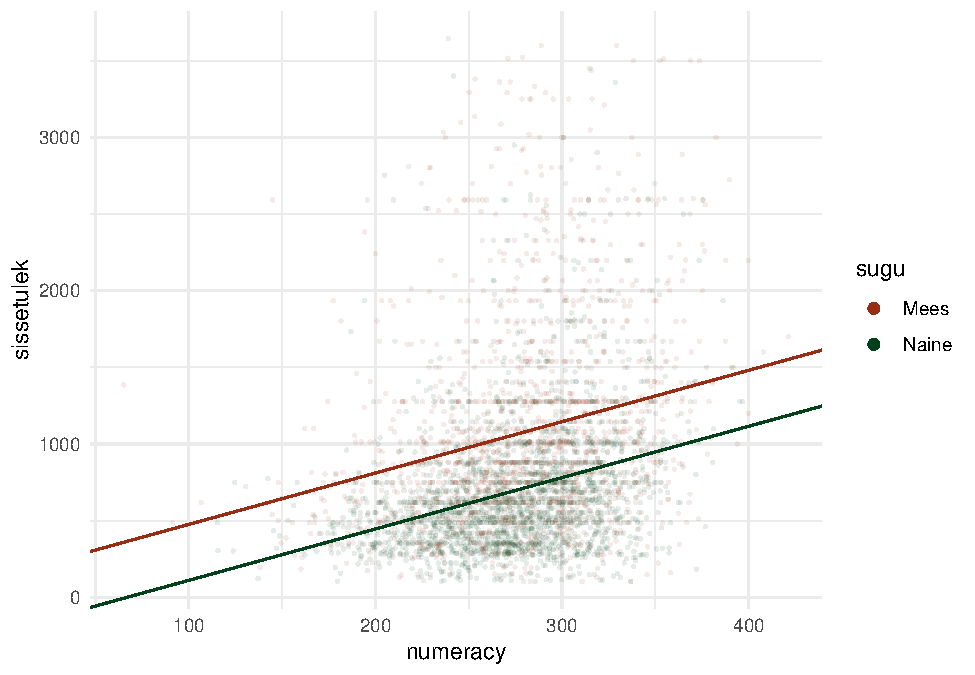
\includegraphics{01-regressioon_files/figure-latex/reg-plot-7-1.pdf}

Lihtsam võimalus seoseid graafiliselt esitada on kasutada paketist \texttt{interactions} funktsiooni \texttt{interaction\_plot()}. See on küll mõeldud eelkõige koosmõjude plottimiseks, kuid toimib ka tavalisete seoste kujutamisel.

\begin{Shaded}
\begin{Highlighting}[]
\FunctionTok{library}\NormalTok{(interactions)}
\FunctionTok{interact\_plot}\NormalTok{(mudel4, }\AttributeTok{pred =}\NormalTok{ numeracy, }\AttributeTok{modx =}\NormalTok{ sugu, }\AttributeTok{colors =} \FunctionTok{c}\NormalTok{(}\StringTok{"\#972D15"}\NormalTok{, }\StringTok{"\#02401B"}\NormalTok{))}
\end{Highlighting}
\end{Shaded}

\includegraphics{01-regressioon_files/figure-latex/unnamed-chunk-15-1.pdf}

\hypertarget{kaks-pidevat-suxf5ltumatut-muutujat}{%
\subsection{Kaks pidevat sõltumatut muutujat}\label{kaks-pidevat-suxf5ltumatut-muutujat}}

Vaatame ka olukorda, kus meil on kaks pidevat sõltumatut tunnust - matemaatiline kirjaoskus ja vanus:

\begin{Shaded}
\begin{Highlighting}[]
\NormalTok{mudel5 }\OtherTok{\textless{}{-}} \FunctionTok{lm}\NormalTok{(sissetulek}\SpecialCharTok{\textasciitilde{}}\NormalTok{numeracy}\SpecialCharTok{+}\NormalTok{vanus, }\AttributeTok{data =}\NormalTok{ piaac)}
\FunctionTok{summary}\NormalTok{(mudel5)}
\end{Highlighting}
\end{Shaded}

\begin{verbatim}
## 
## Call:
## lm(formula = sissetulek ~ numeracy + vanus, data = piaac)
## 
## Residuals:
##     Min      1Q  Median      3Q     Max 
## -1036.6  -349.5  -128.9   178.7  2944.0 
## 
## Coefficients:
##             Estimate Std. Error t value Pr(>|t|)    
## (Intercept)  25.3372    67.3417   0.376    0.707    
## numeracy      3.4841     0.2033  17.137  < 2e-16 ***
## vanus        -3.2210     0.7138  -4.512 6.59e-06 ***
## ---
## Signif. codes:  0 '***' 0.001 '**' 0.01 '*' 0.05 '.' 0.1 ' ' 1
## 
## Residual standard error: 554.5 on 3981 degrees of freedom
##   (3648 observations deleted due to missingness)
## Multiple R-squared:  0.07879,    Adjusted R-squared:  0.07833 
## F-statistic: 170.3 on 2 and 3981 DF,  p-value: < 2.2e-16
\end{verbatim}

Tõlgendame seda järmiselt:

\begin{enumerate}
\def\labelenumi{\arabic{enumi}.}
\tightlist
\item
  Kui matemaatiline kirjaoskus tõuseb ühe punkti võrra, siis sissetulek tõuseb \(3.48\) euro võrra, hoides vanust konstantsena (st see seos kehtib kõikide vanuste jaoks).\\
\item
  Kui vanus tõuseb ühe aasta võrra, siis sissetulek langeb \(3.2\) euro võrra, hoides funktsionaalset lugemisoskust konstantsena (st see seos kehtib kogu funktsionaalse lugemisoskuse skaala ulatuses).\\
\item
  Juhul kui nii vanus oleks \(0\) aastat ja matemaatiline kirjaoskus oleks \(0\) punkti, oleks sissetulek \(25.3\) eurot (kuna selline olukord on suhteliselt võimatu, siis me sellistel puhkudel vabaliiget ei interpreteeri).
\end{enumerate}

Et taolisest mudelist paremini aru saada võime kasutada 3D punktdiagrammi

\begin{Shaded}
\begin{Highlighting}[]
\CommentTok{\#library(car)}
\CommentTok{\#scatter3d(piaac$numeracy,piaac$sissetulek, piaac$vanus)}
\end{Highlighting}
\end{Shaded}

\begin{itemize}
\tightlist
\item
  Looge regressioonimudel, millega hindate \emph{numeracy}, \emph{vanus}, \emph{sugu} ja \emph{haridustase} mõju sissetulekule.
\item
  Milliste tunnuste mõju sissetulekule on statistiliselt oluline?
\item
  Esitage vanuse ja soo mõju sissetulekule graafiliselt.
\end{itemize}

\hypertarget{koosmuxf5jud}{%
\section{Koosmõjud}\label{koosmuxf5jud}}

Eelnevas näites vaatasime sissetuleku sõltuvust matemaatilise kirjaoskuse tasemest soo lõikes, ja nägime, et kui lisame mudelisse soo tunnuse, siis saame klasside kohta eraldi regressioonijooned. Kuid need regressioonijooned olid paralleelsed, mis tähendab et nii meeste kui naiste hulgas oli funktsionaalse lugemisoskuse ja matemaatilise kirjaoskuse suhe mudeli järgi sama. Kuid kas see on alati väga realistlik eeldus? Võib ju vabalt olla, et see seos erineb soo lõikes.

Kui me arvame, et see võib nii olla, st sõltumatu tunnuse mõju sõltuvale tunnusele sõltub omakorda mingist muust tunnusest, saame mudelisse lisada nende kahe tunnuse koosmõju (interaktsiooni). Selleks peame moodustame uue tunnuse, mis tuleneb nende tunnuste, mille suhtes me koosmõju hinnata tahame, korrutisest. Kui me nüüd selle uue tunnuse mudelisse kaasame, siis hindame sellele ka regressioonikoefitsiendi. Regressioonivõrrand pidevtunnuse ja kategoriaalse tunnuse koosmõjuga näeks välja nii:

\[\hat{y}_{sissetulek}=\beta_0+\beta_1 \times numeracy + \beta_2 \times naine + \beta_3 \times naine \times numeracy =\]

\[ 
=
  \begin{cases}
    \beta_0+\beta_1 \times numeracy + \beta_2 \times 1 + \beta_3 \times 1 \times numeracy = (\beta_0+\beta_2)+(\beta_1+\beta_3) \times numeracy  & \quad \text{naised}\\
    \beta_0+\beta_1 \times numeracy + \beta_2 \times 0 + \beta_3 \times 0 \times numeracy = \beta_0+\beta_1 \times numeracy & \quad \text{mehed}
  \end{cases}
\]

R-is saame taolise mudeli defineerida järgmiselt:

\begin{Shaded}
\begin{Highlighting}[]
\NormalTok{mudel8 }\OtherTok{\textless{}{-}} \FunctionTok{lm}\NormalTok{(sissetulek }\SpecialCharTok{\textasciitilde{}}\NormalTok{ numeracy }\SpecialCharTok{*}\NormalTok{ sugu, }\AttributeTok{data =}\NormalTok{ piaac)}
\FunctionTok{summary}\NormalTok{(mudel8)}
\end{Highlighting}
\end{Shaded}

\begin{verbatim}
## 
## Call:
## lm(formula = sissetulek ~ numeracy * sugu, data = piaac)
## 
## Residuals:
##      Min       1Q   Median       3Q      Max 
## -1213.35  -322.79   -99.79   166.87  2802.32 
## 
## Coefficients:
##                     Estimate Std. Error t value Pr(>|t|)    
## (Intercept)          28.4609    79.7161   0.357   0.7211    
## numeracy              3.7552     0.2815  13.340   <2e-16 ***
## suguNaine          -157.9875   107.6870  -1.467   0.1424    
## numeracy:suguNaine   -0.7476     0.3840  -1.947   0.0516 .  
## ---
## Signif. codes:  0 '***' 0.001 '**' 0.01 '*' 0.05 '.' 0.1 ' ' 1
## 
## Residual standard error: 525.8 on 3980 degrees of freedom
##   (3648 observations deleted due to missingness)
## Multiple R-squared:  0.1718, Adjusted R-squared:  0.1712 
## F-statistic: 275.2 on 3 and 3980 DF,  p-value: < 2.2e-16
\end{verbatim}

\begin{Shaded}
\begin{Highlighting}[]
\CommentTok{\# Sama tulemuse saaksime, kui kirjutaksime:}
\CommentTok{\#lm(numeracy \textasciitilde{} literacy + sugu + literacy:sugu, data = piaac)}
\end{Highlighting}
\end{Shaded}

Koosmõjudega mudeli vabaliikmed ja regressioonikoefitsiendid kujunevad järgmiselt:

\[\hat{y}_{sissetulek}=\beta_0+\beta_1 \times numeracy + \beta_2 \times naine + \beta_3 \times naine \times numeracy =\]

\[ 
=
  \begin{cases}
    28.5+3.8 \times numeracy + (-157) \times 1 + (-0.7) \times 1 \times numeracy = (28.5-157)+(3.8-0.7) \times numeracy  & \quad \text{naised}\\
    28.5+3.8 \times numeracy + (-157) \times 0 + (-0.7) \times 0 \times numeracy = 28.5+3.8 \times numeracy & \quad \text{mehed}
  \end{cases}
\]

Seega selles mudelis erinevad kategoriaalse tunnuse lõikes nii vabaliikme väärtused kui ka regressioonisirge tõusud. Kui me nüüd selle mudeli tulemused graafikule paneme, siis näeme, et regressioonisirged ei ole enam paralleelsed. Mida suurem on matemaatilise kirjaoskuse tase, seda suurem on erinevus meeste ja naiste sissetulekutes.

\begin{Shaded}
\begin{Highlighting}[]
\FunctionTok{interact\_plot}\NormalTok{(mudel8, }\AttributeTok{pred =}\NormalTok{ numeracy, }\AttributeTok{modx =}\NormalTok{ sugu,  }\AttributeTok{colors =}  \FunctionTok{c}\NormalTok{(}\StringTok{"\#972D15"}\NormalTok{, }\StringTok{"\#02401B"}\NormalTok{))}
\end{Highlighting}
\end{Shaded}

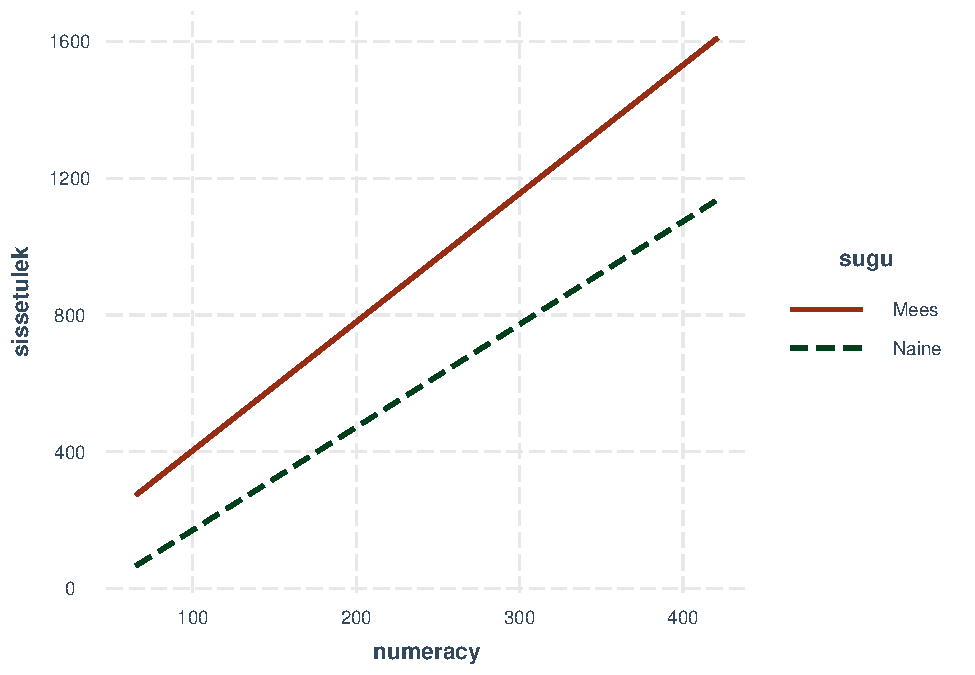
\includegraphics{01-regressioon_files/figure-latex/reg-plot-8-1.pdf}

\hypertarget{koosmuxf5jud-kategoriaalsete-tunnuste-puhul}{%
\subsection{Koosmõjud kategoriaalsete tunnuste puhul}\label{koosmuxf5jud-kategoriaalsete-tunnuste-puhul}}

Enne oli juttu, et kahe kategoriaalse sõltumatu tunnusega mudel ilma koosmõjudeta pole väga mõistlik. Vaatame nüüd kuidas see koosmõjudega välja näeks:

\begin{Shaded}
\begin{Highlighting}[]
\NormalTok{mudel9 }\OtherTok{\textless{}{-}} \FunctionTok{lm}\NormalTok{(sissetulek }\SpecialCharTok{\textasciitilde{}}\NormalTok{ sugu }\SpecialCharTok{*}\NormalTok{ haridustase, }\AttributeTok{data =}\NormalTok{ piaac)}
\FunctionTok{summary}\NormalTok{(mudel9)}
\end{Highlighting}
\end{Shaded}

\begin{verbatim}
## 
## Call:
## lm(formula = sissetulek ~ sugu * haridustase, data = piaac)
## 
## Residuals:
##      Min       1Q   Median       3Q      Max 
## -1126.25  -311.40   -99.32   163.85  2639.98 
## 
## Coefficients:
##                            Estimate Std. Error t value Pr(>|t|)    
## (Intercept)                 1004.53      17.95  55.967   <2e-16 ***
## suguNaine                   -458.80      24.76 -18.533   <2e-16 ***
## haridustaseKõrge             252.60      28.59   8.836   <2e-16 ***
## haridustaseMadal             -73.55      37.63  -1.955   0.0507 .  
## suguNaine:haridustaseKõrge    50.69      36.65   1.383   0.1667    
## suguNaine:haridustaseMadal    10.76      56.52   0.190   0.8491    
## ---
## Signif. codes:  0 '***' 0.001 '**' 0.01 '*' 0.05 '.' 0.1 ' ' 1
## 
## Residual standard error: 526.1 on 3978 degrees of freedom
##   (3648 observations deleted due to missingness)
## Multiple R-squared:  0.1715, Adjusted R-squared:  0.1705 
## F-statistic: 164.7 on 5 and 3978 DF,  p-value: < 2.2e-16
\end{verbatim}

Sellisest mudelist saame välja lugeda kõikide gruppide ristlõigete (kõrge haridustasemega naised, kõrge haridustasemega mehed jne) keskmised. Arvutame näiteks välja kõrge haridustasemega naiste ja madala haridustasemega meeste keskmised matemaatilise lugemisoskuse skoorid:

\[\hat{y}_{sissetulek}=\beta_0+\beta_1 \times naine + \beta_2 \times korge + \beta_3 \times madal + \beta4 \times nainekorge + \beta_5 \times nainemadal =\]

\[ 
=
  \begin{cases}
    1004.5+(-458.8) \times 1 + 252.60 \times 1 + (-73.55) \times 0 + 50.69 \times 1 + 10.76 \times 0 = & \quad \text{kõrge haridustasemega naised}\\
    1004.5+(-458.8) \times 0 + 252.60 \times 0 + (-73.55) \times 1 + 50.69 \times 0 + 10.76 \times 0 = & \quad \text{madala haridustasemega mehed}
  \end{cases}
\]

\[ 
=
  \begin{cases}
    1004.5+(-458.8) + 252.60 + 50.69 =  849 & \quad \text{kõrge haridustasemega naised}\\
    1004.5 + (-73.55) = 931 & \quad \text{madala haridustasemega mehed}
  \end{cases}
\]

Vaatame seda mudelit ka graafiliselt (kasutame paketi \texttt{jtools} funktsiooni \texttt{cat\_plot()}):

\begin{Shaded}
\begin{Highlighting}[]
\FunctionTok{cat\_plot}\NormalTok{(mudel9, }\AttributeTok{pred =}\NormalTok{ haridustase, }\AttributeTok{modx =}\NormalTok{ sugu, }\AttributeTok{colors =}  \FunctionTok{c}\NormalTok{(}\StringTok{"\#972D15"}\NormalTok{, }\StringTok{"\#02401B"}\NormalTok{))}
\end{Highlighting}
\end{Shaded}

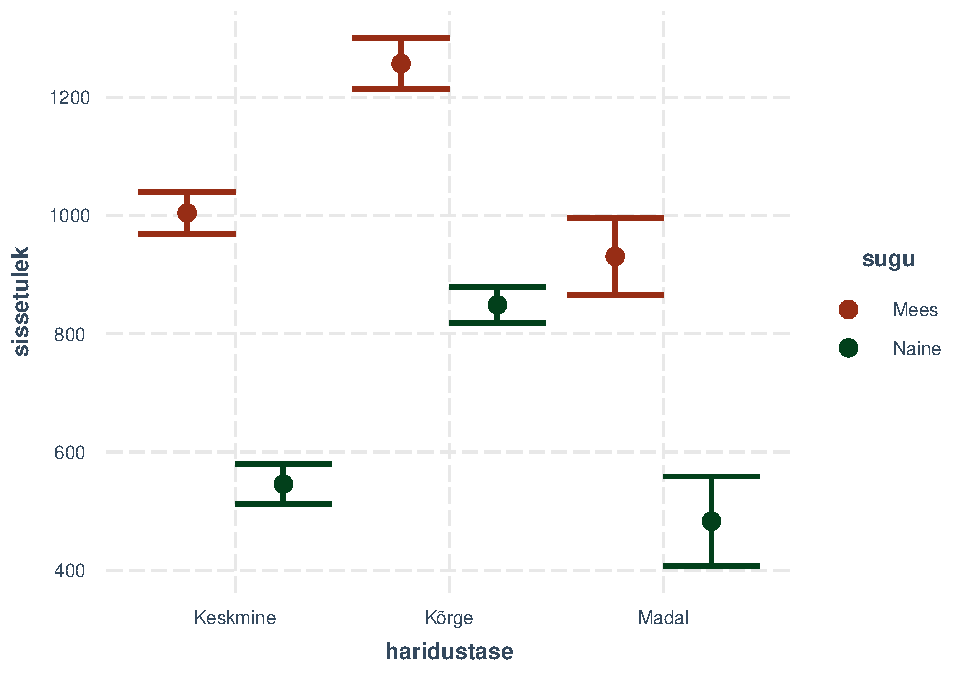
\includegraphics{01-regressioon_files/figure-latex/unnamed-chunk-20-1.pdf}

\begin{itemize}
\tightlist
\item
  Looge koosmõjuga regressioonimudel, millega hindate soo ja laste olemasolu mõju sissetulekule.
\item
  Esitage koosmõjud graafikul (\texttt{cat\_plot()} abiga)
\end{itemize}

\hypertarget{mudelite-vuxf5rdlemine}{%
\section{Mudelite võrdlemine}\label{mudelite-vuxf5rdlemine}}

Milline on hea mudel? See peaks muidugi seletama võimalikult palju sõltuva tunnuse varieeruvusest. Samas peaks see olema ka võimalikult ökonoomne, st see peaks sisaldama ainult tunnuseid, mis mudelit oluliselt paremaks teevad. Siin on rõhk sõnal ``oluliselt''. Iga lisanduv tunnus teeb mudeli mingil määral paremaks, kuid see paranemine võib olla mikroskoopiline. Kuidas siis hinnata, kas mudel \(n+1\) tunnusega on oluliselt parem kui \(n\) tunnusega mudel?

Me saame vaadata lisanduva tunnuse standardviga, \emph{t}-väärtust ja sellega seonduvat \emph{p}-väärtust. Kuid nagu enne jutuks oli, testib see ainult konkreetse koefitsiendi erinevust nullist. Meid aga huvitab kogu mudeli kvaliteet. Võimalus on ka võrrelda mudelite \(R^2\) väärtusi, kuid need on pigem kirjeldavad, ega anna meile indikatsiooni sellest kas üks väärtus on oluliselt parem kui teine.

Erinevate mudelite statistiliselt olulist erinevust saame testida hii-ruut testiga kasutades \texttt{anova()} funktsiooni. Seda saab teha ainult siis kui mudelid on omavehl seotud (\emph{nested}), st keerukam (rohkemate tunnustega) mudel peab sisdaldama kõiki lihtsama mudeli tunnuseid.

\begin{Shaded}
\begin{Highlighting}[]
\NormalTok{mudel\_test1 }\OtherTok{\textless{}{-}} \FunctionTok{lm}\NormalTok{(numeracy }\SpecialCharTok{\textasciitilde{}}\NormalTok{ literacy, }\AttributeTok{data =}\NormalTok{ piaac)}
\NormalTok{mudel\_test2 }\OtherTok{\textless{}{-}} \FunctionTok{lm}\NormalTok{(numeracy }\SpecialCharTok{\textasciitilde{}}\NormalTok{ literacy }\SpecialCharTok{+}\NormalTok{ sugu, }\AttributeTok{data =}\NormalTok{ piaac)}
\FunctionTok{anova}\NormalTok{(mudel\_test1, mudel\_test2, }\AttributeTok{test =} \StringTok{"Chisq"}\NormalTok{)}
\end{Highlighting}
\end{Shaded}

\begin{verbatim}
## Analysis of Variance Table
## 
## Model 1: numeracy ~ literacy
## Model 2: numeracy ~ literacy + sugu
##   Res.Df     RSS Df Sum of Sq  Pr(>Chi)    
## 1   7584 4848657                           
## 2   7583 4734885  1    113772 < 2.2e-16 ***
## ---
## Signif. codes:  0 '***' 0.001 '**' 0.01 '*' 0.05 '.' 0.1 ' ' 1
\end{verbatim}

Tõlgendame jällegi testi \emph{p}-väärtust. Kui see on väiksem kui \(0.05\) (usaldusnivool \(95\%\)), siis võime järeldada, et mudelid on oluliselt erinevad, mis tähendab omakorda, et lisatud tunnus tõstis mudeli selgitusvõimet olulisel määral.

\hypertarget{regressioonimudeli-eeldused}{%
\section{Regressioonimudeli eeldused}\label{regressioonimudeli-eeldused}}

Nagu iga meetodi puhul, on ka lineaarsel regressioonanalüüsil rida eeldusi, mis peavad olema täidetud, et analüüsist korrektseid järeldusi oleks võimalik teha.

\begin{enumerate}
\def\labelenumi{\arabic{enumi}.}
\tightlist
\item
  Esimene ja vahest ka kõige olulisem eeldus on \textbf{lineaarne suhe sõltuva ja sõltumatu(te) tunnuse vahel}. Kõrvaloleval joonisel on esitatud neli andmestikku, mille regressioonisirged on identsed (\(y=3+0.5x\)). Tegelikult on identsed ka kõik muud andmete statistilised omadused (\(x\)'i keskmine, \(y\)'i keskmine, \(x\)'i dispersioon, \(y\)'i dispersioon ja ka korrelatsioon). Ometi on visuaalselt näha, et kõik andmestikud on väga erinevad. Seega peaks regressioonanalüüsi (või tegelikult ükskõik mis analüüsi) puhul olema alati esimene samm neid graafiliselt uurida. Kui tunnuste vaheline seos ei ole lineaarne, piisab mõnel juhul tunnuste mittelineaarsest transformeerimisest (see peaks olema ka muidugi teoreetiliselt põhjendatud). Kui seos on eksponentsiaalne, siis võib kaaluda \emph{log}-transformatsiooni. Kui seos on paraboolne, siis võib kaaluda ruutu tõstetud tunnuse lisamist (\(y = \beta_0+\beta_1x+\beta_2x^2\)). Taoliste transformatsioonide juures peab meeles pidama, et koos nendega muutub ka mudeli tõlgendus.
\end{enumerate}

\begin{figure}
\centering
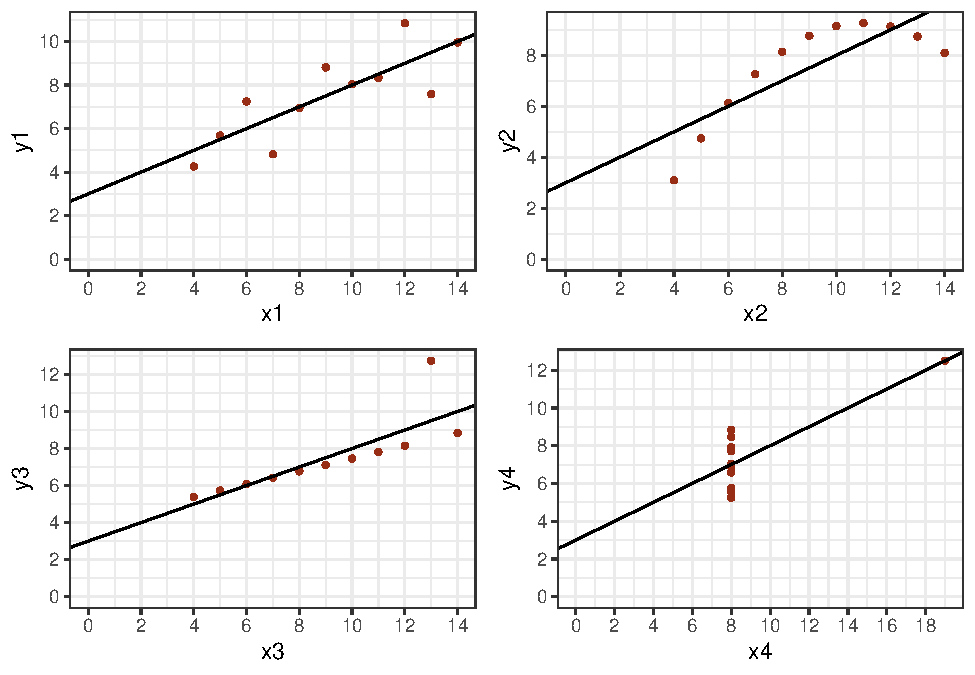
\includegraphics{01-regressioon_files/figure-latex/anscombe-1.pdf}
\caption{\label{fig:anscombe}Anscombe kvartett}
\end{figure}

\begin{enumerate}
\def\labelenumi{\arabic{enumi}.}
\setcounter{enumi}{1}
\item
  Lineaarse regressiooni puhul peaks tähelepanelik olema ka \textbf{erindite} (\emph{outliers})suhtes, st vaatluste suhtes, mis erinevad teistest väga olulisel määral (nagu ka kõrvalolevalt jooniselt näha). Mõnede andmete puhul on erindid paratamatud (näiteks sissetuleku puhul, kus suurem osa inimesi on koondunud keskmise sissetuleku ümber, kuid mõned üksikud teenivad sellest oluliselt enam). Sellisel juhul tasuks kaaluda jällegi tunnuse transformeerimist (sissetuleku puhul näiteks log-skaalale). Kui tegemist on mõne üksiku erindiga, võiks ju selle aluseks oleva vaatluse ka lihtsalt analüüsist välja jätta. Siin tuleks aga olla väga ettevaatlik. Andmete või sellest saadava informatsiooni tahtlik vähendamine (näiteks pidevtunnuste kategoriseerimine) ei ole üldiselt kunagi hea mõte. Seda enam ei ole hea mõte andmete vähendamine eesmärgiga mudelit paremaks teha. Kui aga erindite tekkimine on mingil moel teoreetiliselt seletatav või tulenenud näiteks veast andmekorjel, siis võib seda loomulikult teha.
\item
  \textbf{Jääkide dispersiooni homogeensus} (\emph{homoscedasticity}). Jäägid peaksid hinnatud väärtuste lõikes olema homogeense ja konstantse variatiivsusega, st ühtlaselt jaotunud kõikide \(\hat{y}\) väärtuste ümber. Selle eelduse rikkumine mõjutab eelkõige standardvigu (need ei kehti enam kõikidele \(\hat{y}\) väärtustele ühtlaselt) ja seeläbi loomulikult ka usalduintervalle ning \emph{p}-väärtusi. Lahenduseks võivad olla nn robustsed standardvead (\emph{robust standard errors}), mis võtavad varieeruvuse erinevust arvesse.
\end{enumerate}

\begin{Shaded}
\begin{Highlighting}[]
\DocumentationTok{\#\# Robust standard errors}
\NormalTok{mudel6 }\OtherTok{\textless{}{-}} \FunctionTok{lm}\NormalTok{(numeracy }\SpecialCharTok{\textasciitilde{}}\NormalTok{ literacy }\SpecialCharTok{*}\NormalTok{ sugu, }
             \AttributeTok{data =}\NormalTok{ piaac)}

\CommentTok{\# Tavalised standardvead}
\FunctionTok{summary}\NormalTok{(mudel6)}
\end{Highlighting}
\end{Shaded}

\begin{verbatim}
## 
## Call:
## lm(formula = numeracy ~ literacy * sugu, data = piaac)
## 
## Residuals:
##      Min       1Q   Median       3Q      Max 
## -102.441  -16.551   -0.094   16.867   88.714 
## 
## Coefficients:
##                     Estimate Std. Error t value Pr(>|t|)    
## (Intercept)        36.129029   2.620050  13.789  < 2e-16 ***
## literacy            0.871523   0.009417  92.543  < 2e-16 ***
## suguNaine           4.596729   3.619797   1.270 0.204164    
## literacy:suguNaine -0.044937   0.012972  -3.464 0.000535 ***
## ---
## Signif. codes:  0 '***' 0.001 '**' 0.01 '*' 0.05 '.' 0.1 ' ' 1
## 
## Residual standard error: 24.97 on 7582 degrees of freedom
##   (46 observations deleted due to missingness)
## Multiple R-squared:  0.6948, Adjusted R-squared:  0.6946 
## F-statistic:  5753 on 3 and 7582 DF,  p-value: < 2.2e-16
\end{verbatim}

\begin{Shaded}
\begin{Highlighting}[]
\CommentTok{\# Robustsed standardvead}
\FunctionTok{library}\NormalTok{(sandwich)}
\FunctionTok{library}\NormalTok{(lmtest)}

\FunctionTok{coeftest}\NormalTok{(mudel6, }\AttributeTok{vcov. =} \FunctionTok{vcovHC}\NormalTok{(mudel6))}
\end{Highlighting}
\end{Shaded}

\begin{verbatim}
## 
## t test of coefficients:
## 
##                      Estimate Std. Error t value  Pr(>|t|)    
## (Intercept)        36.1290294  2.7887350 12.9553 < 2.2e-16 ***
## literacy            0.8715229  0.0098976 88.0538 < 2.2e-16 ***
## suguNaine           4.5967288  3.8313081  1.1998 0.2302621    
## literacy:suguNaine -0.0449372  0.0135552 -3.3151 0.0009203 ***
## ---
## Signif. codes:  0 '***' 0.001 '**' 0.01 '*' 0.05 '.' 0.1 ' ' 1
\end{verbatim}

\begin{Shaded}
\begin{Highlighting}[]
\CommentTok{\# Saab ka nii}
\FunctionTok{library}\NormalTok{(sandwich)}
\FunctionTok{vcovHC}\NormalTok{(mudel6) }\SpecialCharTok{\%\textgreater{}\%} 
  \FunctionTok{diag}\NormalTok{() }\SpecialCharTok{\%\textgreater{}\%} 
  \FunctionTok{sqrt}\NormalTok{()}
\end{Highlighting}
\end{Shaded}

\begin{verbatim}
##        (Intercept)           literacy          suguNaine literacy:suguNaine 
##        2.788735004        0.009897618        3.831308067        0.013555193
\end{verbatim}

\begin{enumerate}
\def\labelenumi{\arabic{enumi}.}
\setcounter{enumi}{3}
\item
  \textbf{Jääkide normaaljaotus}. Regressiooni jäägid peaksid olema normaaljaotusega \(e_i \sim N(0, \sigma^2)\), seega enamus jääke peaks jääma nulli ümber ning mida suuremad jäägid, seda vähem neid olema peaks. See eeldus on eelkõige oluline regressioonikoefitsientide \emph{t}-testi jaoks.
\item
  \textbf{Jääkide sõltumatus}. Ühe vaatluse jäägid ei tohiks olla korreleeritud teise vaatluse jääkidega. Selline olukord võib tekkida näiteks siis kui meil mudelist välja jäänud mingi oluline tunnus (ühe tunnuse regressiooni puhul on see muidugi vaid hüpoteetiline olukord), näiteks hindame õpilaste testiskoore lähtuvalt nende õppimisele kulunud ajast, kuid ei arvesta, et õpilased tulevad näiteks erinevatest koolidest, kus võib olla erinev tase. Seega õpilaste tulemused ei ole enam sõltumatud, vaid sõltuvad koolist. Regressioonikoefitsientide standardvigade arvutamisel lähtutakse eeldusest, et jäägid on sõltumatud. Kui jäägid on korreleeritud, siis võib juhtuda, et me alahindame standardvigade suurust ehk siis oleme oma tulemustes ülemäära kindlad (usaldusintervallid ning \emph{p}-väärtused tulevad liialt väikesed) ning võime näha seoseid seal kus neid tegelikult ei ole. Lahenduseks võiks olla puuduolevate tunnuste lisamine mudelisse (konkrteetse näite puhul kooli tunnus).
\item
  Kui kaks sõltumatut tunnust on teineteisega väga tugevalt seotud põhjusteab see nn \textbf{kollineaarsust}. See võib tekitada probleeme mudeli hindamisel ning ka tõlgendusel. Lisaks kipuvad standardvead liialt suureks minema, mis tähendab seda, et kaotame oma tulemuste täpsuses ja võime mitte näha seoseid seal, kus need tegelikult olemas on. Seega võiks tähele panna, et korrelatsioon sõltumatute muutujate vahel peaks alati olema väiksem kui korrelatsioon sõltuva ja sõltumatu muutuja vahel.
\end{enumerate}

\hypertarget{kuidas-eelduste-tuxe4idetust-hinnata}{%
\section{Kuidas eelduste täidetust hinnata?}\label{kuidas-eelduste-tuxe4idetust-hinnata}}

Eelduste hindamiseks on loomulikult mitmeid teste, kuid kõige lihtsam on seda mudeli diagnostiliste joonistega.

\begin{Shaded}
\begin{Highlighting}[]
\NormalTok{mod }\OtherTok{\textless{}{-}} \FunctionTok{lm}\NormalTok{(}\AttributeTok{formula =}\NormalTok{ sissetulek }\SpecialCharTok{\textasciitilde{}}\NormalTok{ numeracy }\SpecialCharTok{+}\NormalTok{ vanus }\SpecialCharTok{+}\NormalTok{ sugu }\SpecialCharTok{+}\NormalTok{ haridustase, }
    \AttributeTok{data =}\NormalTok{ piaac)}
\end{Highlighting}
\end{Shaded}

\begin{Shaded}
\begin{Highlighting}[]
\FunctionTok{plot}\NormalTok{(mod, }\DecValTok{1}\NormalTok{)}
\end{Highlighting}
\end{Shaded}

\includegraphics{01-regressioon_files/figure-latex/unnamed-chunk-24-1.pdf}
Kontrollime mittelineaarse seose olemasolu. Punktid peaksid olema ühtlaselt ümber keskmise joone jaotunud. Ei tohiks olla mingit ilmset mustrit.

\begin{Shaded}
\begin{Highlighting}[]
\FunctionTok{plot}\NormalTok{(mod, }\DecValTok{2}\NormalTok{)}
\end{Highlighting}
\end{Shaded}

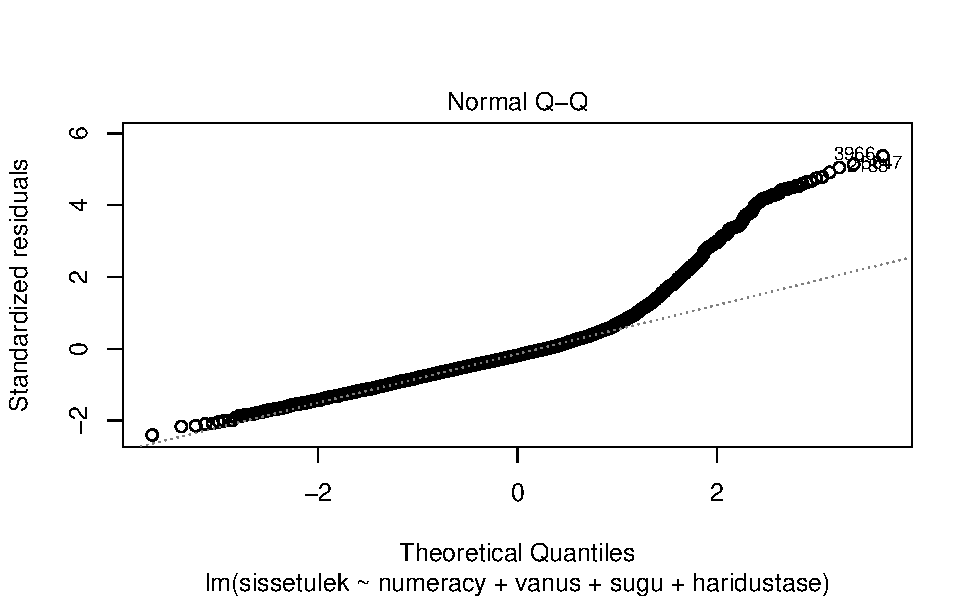
\includegraphics{01-regressioon_files/figure-latex/unnamed-chunk-25-1.pdf}
Kas jäägid on normaalselt jaotunud? Punktid peaksid ühtima diagonaalse joonega.

\begin{Shaded}
\begin{Highlighting}[]
\FunctionTok{plot}\NormalTok{(mod, }\DecValTok{3}\NormalTok{)}
\end{Highlighting}
\end{Shaded}

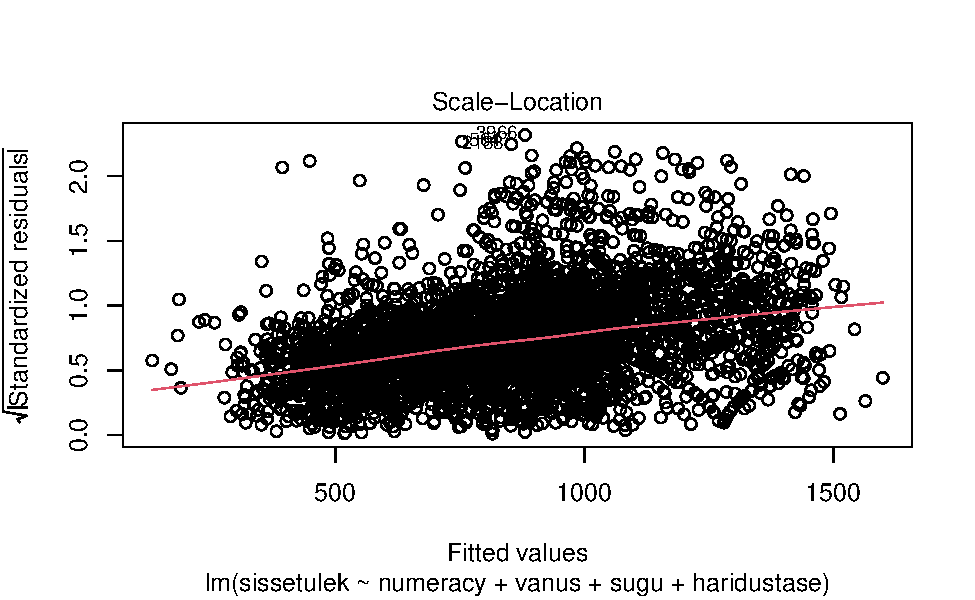
\includegraphics{01-regressioon_files/figure-latex/unnamed-chunk-26-1.pdf}
Kas jääkide dispersioon on homogeenne? Punane joon peaks olema horisontaalne ja punktid peaksid olema ühtlaselt jaotunud ega tohiks mingit mustrit moodustada.

\begin{Shaded}
\begin{Highlighting}[]
\FunctionTok{plot}\NormalTok{(mod, }\DecValTok{5}\NormalTok{)}
\end{Highlighting}
\end{Shaded}

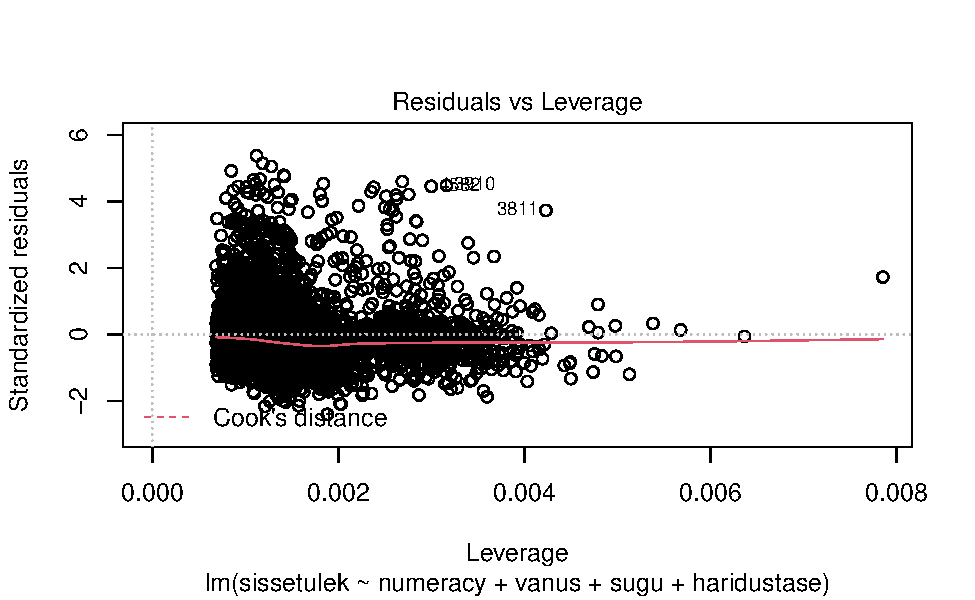
\includegraphics{01-regressioon_files/figure-latex/unnamed-chunk-27-1.pdf}
Kas mudelis on mudelit oluliselt mõjutavaid erindeid? Kui on, siis peaksid need olema paremal all või paremal üleval nurgas ning kaugemal kui punktiirjoon (antud juhul neid ei ole ja seega ei ole ka punktiirjoont näha).

\hypertarget{part-uxfcldistatud-lineaarsed-mudelid}{%
\part{Üldistatud lineaarsed mudelid}\label{part-uxfcldistatud-lineaarsed-mudelid}}

\hypertarget{logistiline-regressioon}{%
\chapter{Logistiline regressioon}\label{logistiline-regressioon}}

Logistilise regressiooniga (logit-mudeliga) saame hinnata sõltumatute tunnuste mõju binaarsele sõltuvale tunnusele (töötav/töötu, käis valimas/ei käinud valimas, surnud/ei ole surnud). Teisisõnu, hindame tõenäosust mingi sündmuse toimumiseks (\emph{success}/\emph{failure}). Sõltuva tunnuse \(y\) jaotus on määratletud kui sündmuse toimumise tõenäosus \(P(Y=1)=\pi\).\\
Tavalise regressiooni mudel oli väljendatav kui \(\bar{y}=\beta_0+\beta_p x_p\). Miks me ei võiks pidevtunnuselise \(y\) keskmist asendada \(\pi\)'ga: \(\bar{\pi}=\beta_0+\beta_k x_k\)? Aga sellepärast, et tõenäosus on piiritletud \(0\) ja \(1\)'ga, samas kui lineaarne funktsioon hõlmab kõiki reaalarvulisi väärtusi. Seega on ülimalt tõenäoline, et mingite \(x\)'i väärtuste puhul on prognoositav \(y\) väärtus suurem kui \(1\) või väiksem kui \(0\). Lisaks tekivad probleemid jääkide struktuuriga (tavaline regressioon eeldab normaaljaotust) ja jääkide dispersiooniga (tavaline regressioon eeldab konstantset hajuvust).

\begin{figure}
\centering
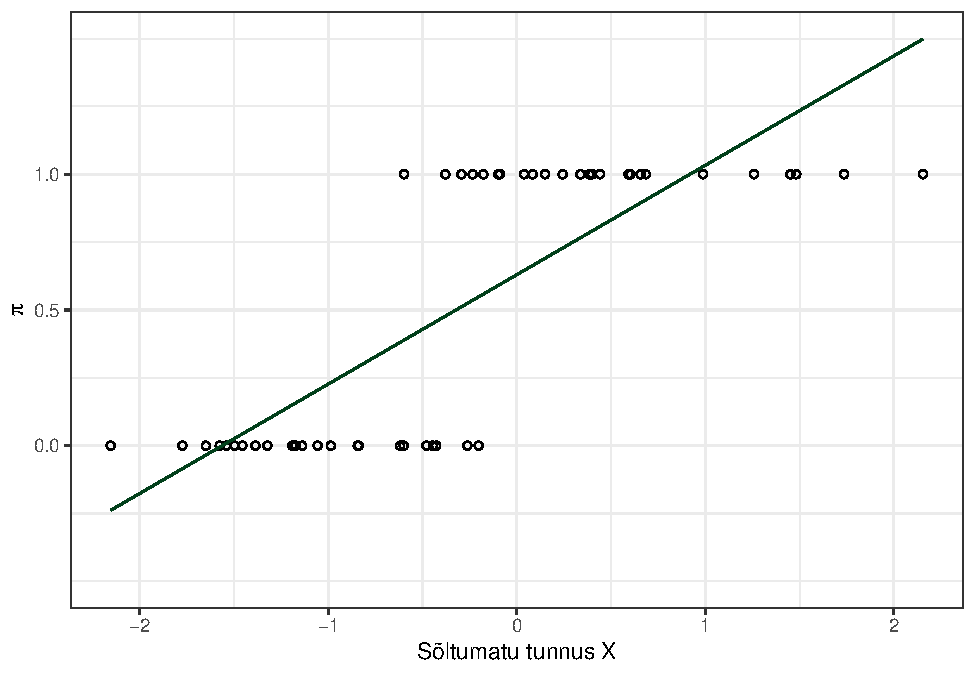
\includegraphics{02-logit_files/figure-latex/glm-1-1.pdf}
\caption{\label{fig:glm-1}Lineaarse regressiooni kasutamine binaarse sõltuva tunnusega}
\end{figure}

\hypertarget{ux161ansid}{%
\section{Šansid}\label{ux161ansid}}

Kuidas me saaksime tõenäosuse skaala (\(0 \dots1\)) teisendada pidevaks skaalaks (\(-\infty \dots \infty\))? Et saada lahti maksimaalsest väärtusest (\(1\)), on võimalik kasutada sündmuse toimumise tõenäosuse asemel sündmuse toimumise šanssi (\emph{odds}). Šanssideks nimetatakse sündmuse toimumise ja mittetoimumise suhet:

\[\text{šansid}=\frac{p}{(1-p)}\]

Näiteks kulli ja kirja viskamisel on kulli saamise šanss \(\frac{0.5}{(1-0.5)}=1\). Šanss võtta kaardipakist ruutu on \(\frac{0.25}{(1-0.25)}=\frac{1}{3}=0.33\).

\begin{figure}
\centering
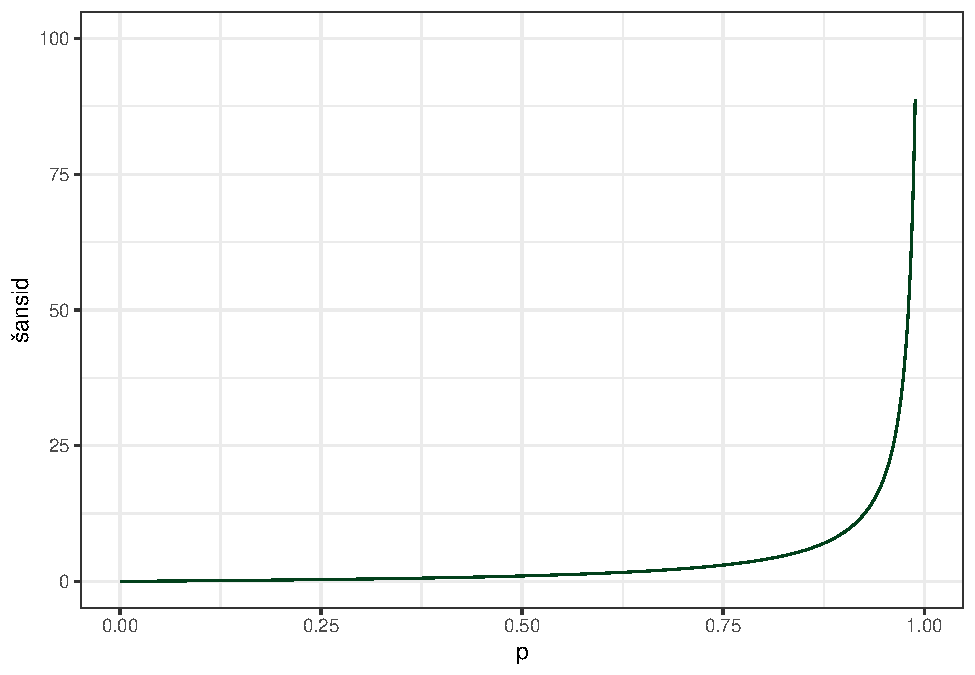
\includegraphics{02-logit_files/figure-latex/odds-1.pdf}
\caption{\label{fig:odds}Šansside ja tõenäosuse suhe}
\end{figure}

Šansid saab omakorda teisenda tagasi tõenäosuseks:

\[p=\frac{\text{šansid}}{1+\text{šansid}}\]

\hypertarget{logit}{%
\section{Logit}\label{logit}}

Kuid tõenäosuse alumine piir jääb sel juhul ikkagi ette. Ka šansid on altpoolt piiratud (nad ei saa olla väiksemad kui \(0\)). Lahenduseks on võtta šansside logaritm. Saadud väärtust nimetatakse \textbf{logit}-iks (\emph{log odds}):

\[\text{logit}=\log \bigg(\frac{p}{(1-p)}\bigg)\]

\begin{figure}
\centering
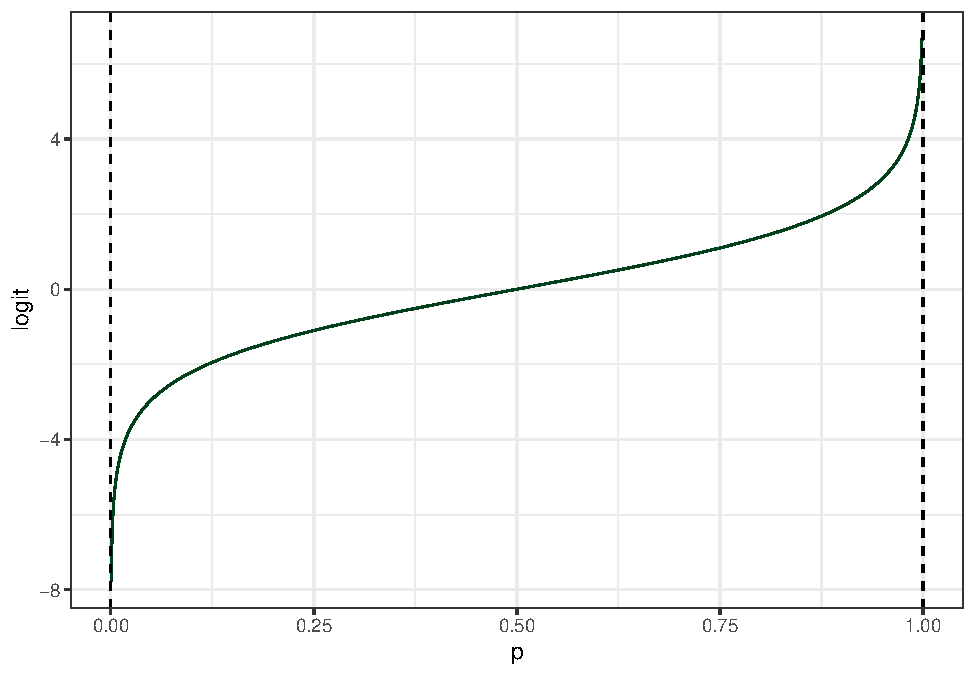
\includegraphics{02-logit_files/figure-latex/glm-3-1.pdf}
\caption{\label{fig:glm-3}Logit-i ja tõenäosuse suhe}
\end{figure}

\hypertarget{logit-mudel}{%
\section{Logit mudel}\label{logit-mudel}}

Lõpuks saame mudeli võrrandi kokku panna:

\[\text{logit}(\pi_i)=\text{log} \left(\dfrac{\pi_i}{1-\pi_i}\right)=\beta_0+\beta_1 x_i\]

Või kui võtame mõlemast poolest eksponendi:

\[\frac{\pi_i}{1-\pi_i}=e^{({\beta_0}+\beta_1 x_i)}\]
Sama võrrandit saab esitada ka nii:

\[\pi_i=Pr(Y_i=1|X_i=x_i)=\dfrac{e^{(\beta_0+\beta_1 x_i)}}{1+e^{(\beta_0+\beta_1 x_i)}}\]\\
või hoopis nii:

\[\pi_i=Pr(Y_i=1|X_i=x_i)=\frac{1}{1+e^{-\beta_0-\beta_1 x_i}}\]

\begin{figure}
\centering
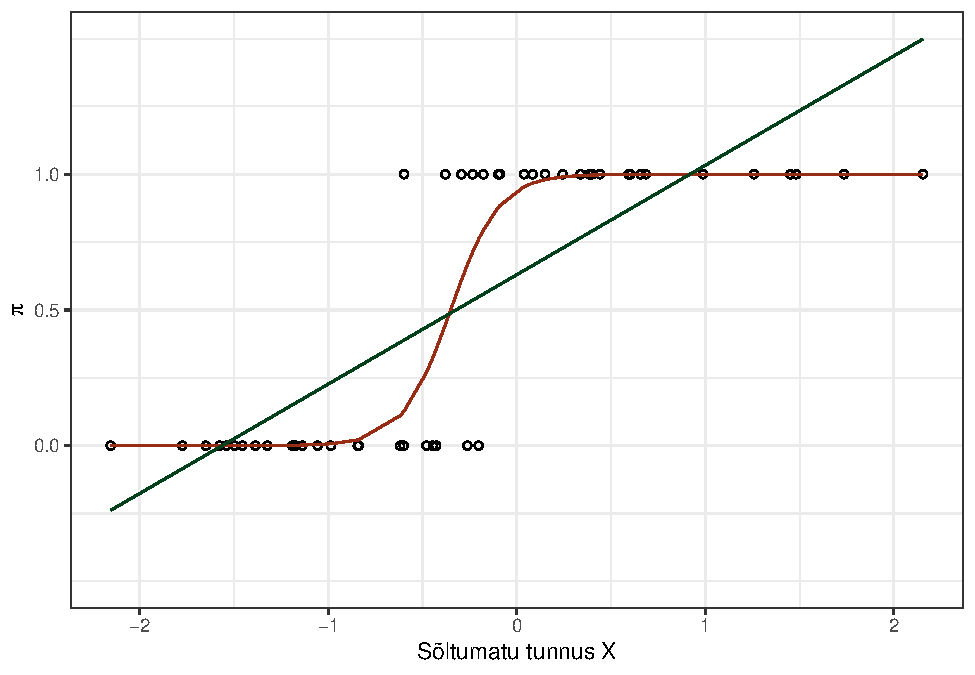
\includegraphics{02-logit_files/figure-latex/glm-2-1.pdf}
\caption{\label{fig:glm-2}Logistiline regressioon võrdluses lineaarse regressiooniga}
\end{figure}

\hypertarget{mudeli-tuxf5lgendus}{%
\section{Mudeli tõlgendus}\label{mudeli-tuxf5lgendus}}

Tavalise regresioonimudeliga saime prognoosida \(y\) väärtust mingite \(x\) väärtuste korral (ja \(y\) muutust, kui \(x\) muutub ühe ühiku võrra). Sama kehtib ka logistilise regressiooni korral. Kuid mida me siinjuures täpsemalt prognoosime? Tahaksime kindlasti prognoosida (uuritava sündmuse toimumise) tõenäosust. Kuid kuna me teisendasime tõenäosuse logititeks, siis tegelikult saame prognoosida hoopis logitit. Ja ka ühe ühikuline muutus \(x\)-is ei peegelda mitte \(y\) tõenäosuse muutust, vaid muutust logit(\(y\))-is. Logiteid ei oska me (vähemalt esialgu) kuidagi tõenäosuslikult tõlgendada. Mida siis teha? Lahenduseks on võtta \emph{logit}-i võrrandi mõlemast poolest eksponent \(exp(logit) = exp(\beta_0+\beta_1 x_i) \implies \frac{\pi_i}{1-\pi_i}=e^{({\beta_0}+\beta_1 x_i)}\). Sellisel juhul saab \(y\)-t tõlgendada kui šansse ja \(\beta\)-t kui muutust šanssides (mitu korda \(x\)-i ühe ühiku muutudes \(y\) šansid suurenevad või vähenevad). Seda šansside muutust väljendavat kordajat nimetatakse šansside suhteks.

\hypertarget{ux161ansside-suhe}{%
\subsection{Šansside suhe}\label{ux161ansside-suhe}}

Šansid saime leida valemiga:

\[\text{šansid}=\frac{p}{(1-p)}\]\\
Valemist võime välja lugeda järgmist:

\begin{enumerate}
\def\labelenumi{\arabic{enumi}.}
\tightlist
\item
  Šansid on alati positiivsed\\
\item
  Kui šansid on \(1\), siis on sündmuse toimumise ja mittetoimumise tõenäosus võrdsed (\(p=0.5\)).\\
\item
  Kui šansid on suuremad kui \(1\), siis on sündmuse toimumise tõenäosus suurem kui mittetoimumise tõenäosus (\(p>0.5\)) ja vastupidi.\\
  Näiteks kui sündmuse toimumise tõenäosus on \(0.8\), siis on šansid \(\frac{0.8}{1-0.8}=\frac{0.8}{0.2}=4\). Seega sündmuse toimumise tõenäosus on \(4\) korda suurem kui selle mittetoimumise tõenäosus. Kui sündmuse toimumise tõenäosus on \(0.2\), siis on šansid \(\frac{0.2}{1-0.2}=\frac{0.2}{0.8}=\frac{1}{4}=0.25\). Sündmuse toimumise tõenäosus on \(4\) korda väiksem kui selle mittetoimumise tõenäosus.
\end{enumerate}

Vaatame näidet, kus hindame hääletamise tõenäosust ning abielu mõju sellele:

\begin{longtable}[]{@{}lll@{}}
\toprule
& Hääletab & Ei hääleta \\
\midrule
\endhead
Abielus & 0.75 & 0.25 \\
Ei ole abielus & 0.54 & 0.46 \\
\bottomrule
\end{longtable}

Abielus inimeste puhul on šanss hääletamiseks \(\frac{0,75}{0,25} = \frac{3}{1}= 3\) (iga mittehääletaja kohta on kolm hääletajat).

Vallaliste puhul on šanss hääletamiseks \(\frac{0,54}{0,46} = 1,17\) (iga mittehääletaja kohta on \(1,17\) hääletajat).

Meid huvitab kuidas sõltumatu tunnuse muutus sündmuse toimumise šansse mõjutab, ehk kui palju muutuvad šansid kui sõltumatu tunnus muutub ühe ühiku võrra. Seda muutust väljendabki šansside suhe (\emph{odds ratio} ehk OR)

\[OR=\frac{y \text{ šanss juhul kui } x \text{ väärtus muutub ühe ühiku võrra}}{y \text{ šanss juhul kui } x \text{ väärtus jääb samaks}}\]

Kui palju on abielus olijate šansid hääletamiseks suuremad kui vallalistel? Šansside suhe on \(\frac{3}{1,17}=2,56\). Ehk siis abielus olijate šanss hääletada on kaks ja pool korda suurem. Abielu tunnuse ühe ühiku muutumisega muutuvad šansid \(2,56\) korda ehk suurenevad \(156\%\).

\hypertarget{logistiline-regressioon-r-is}{%
\section{Logistiline regressioon R-is}\label{logistiline-regressioon-r-is}}

Võtame R-i näidisandmestiku \texttt{Titanic}, mis kirjeldab Titanicul hukkunute ja ellujäänute sugu, vanust ja reisijaklassi. Üritame hinnata kuidas ja kas need tunnused mõjutasid ellujäämist.\\
GLMi mudeleid saab R'is defineerida \texttt{glm()} funktsiooniga. Selle loogika ja argumendid on sarnased \texttt{lm()} funktsiooni omadele. Peamiseks erinevuseks on see, et nüüd peame defineerima ka sõltuva tunnuse jaotuse ja linkfunktsiooni. See käib argumendiga \texttt{family}. Logistilise regressiooni jaoks peame defineerima \texttt{family\ =\ binomial(link\ =\ logit)} (sõltuva tunnuse jaotus on binoomjaotus ja linkfunktsioon on logit).\\
Vaatame kõigepealt soo mõju:

\begin{Shaded}
\begin{Highlighting}[]
\CommentTok{\# Andmestik on algselt tabeli kujul.}

\CommentTok{\# Saaksime seda ka sellisel kujul analüüsida,}
\CommentTok{\# kuid mugavam ja selgem on, kui keerame ta}
\CommentTok{\# nn tavalisele kujule. Kasutame selleks }
\CommentTok{\# paketi tidyr funktsiooni uncount()}

\NormalTok{titanic }\OtherTok{\textless{}{-}}\NormalTok{ datasets}\SpecialCharTok{::}\NormalTok{Titanic }\SpecialCharTok{\%\textgreater{}\%} 
  \FunctionTok{as.data.frame}\NormalTok{() }\SpecialCharTok{\%\textgreater{}\%} 
\NormalTok{  tidyr}\SpecialCharTok{::}\FunctionTok{uncount}\NormalTok{(Freq)}

\CommentTok{\# vaatame andmestiku esimesi ridu}
\FunctionTok{head}\NormalTok{(titanic)}
\end{Highlighting}
\end{Shaded}

\begin{verbatim}
##   Class  Sex   Age Survived
## 1   3rd Male Child       No
## 2   3rd Male Child       No
## 3   3rd Male Child       No
## 4   3rd Male Child       No
## 5   3rd Male Child       No
## 6   3rd Male Child       No
\end{verbatim}

\begin{Shaded}
\begin{Highlighting}[]
\CommentTok{\# Defineerime mudeli}
\NormalTok{mudel7 }\OtherTok{\textless{}{-}} \FunctionTok{glm}\NormalTok{(}\FunctionTok{I}\NormalTok{(Survived }\SpecialCharTok{==} \StringTok{"Yes"}\NormalTok{)}\SpecialCharTok{\textasciitilde{}}\NormalTok{Sex, }\AttributeTok{data =}\NormalTok{ titanic, }\AttributeTok{family =} \FunctionTok{binomial}\NormalTok{())}
\FunctionTok{summary}\NormalTok{(mudel7)}
\end{Highlighting}
\end{Shaded}

\begin{verbatim}
## 
## Call:
## glm(formula = I(Survived == "Yes") ~ Sex, family = binomial(), 
##     data = titanic)
## 
## Deviance Residuals: 
##     Min       1Q   Median       3Q      Max  
## -1.6226  -0.6903  -0.6903   0.7901   1.7613  
## 
## Coefficients:
##             Estimate Std. Error z value Pr(>|z|)    
## (Intercept)  -1.3128     0.0588  -22.32   <2e-16 ***
## SexFemale     2.3172     0.1196   19.38   <2e-16 ***
## ---
## Signif. codes:  0 '***' 0.001 '**' 0.01 '*' 0.05 '.' 0.1 ' ' 1
## 
## (Dispersion parameter for binomial family taken to be 1)
## 
##     Null deviance: 2769.5  on 2200  degrees of freedom
## Residual deviance: 2335.0  on 2199  degrees of freedom
## AIC: 2339
## 
## Number of Fisher Scoring iterations: 4
\end{verbatim}

\begin{Shaded}
\begin{Highlighting}[]
\CommentTok{\# I(Survived == "Yes") notatsiooniga saame tekstilise tunnuse }
\CommentTok{\# teisendada loogilisek tunnuseks }
\CommentTok{\# saaksime seda teha ka näiteks nii:}
\CommentTok{\#   titanic$surv \textless{}{-} titanic$Survived == "Yes"}
\CommentTok{\#   glm(surv\textasciitilde{}Sex, data = titanic, family = binomial())}
\CommentTok{\# Tulemus on sama}
\end{Highlighting}
\end{Shaded}

Väljundist leiame kõigepealt regressioonikoefitsiendid, nende standardvead, z-väärtused ja z-testi \emph{p}-väärtuse\footnote{z-test puhul on tegemist t-testi analoogiga, mis ei lähtu mitte t-jaotusest, vaid normaaljaotusest. Tõlgendus on aga sama}. Kuid koefitsiendid on nüüd logititskaalal ja seepärast küllaltki raskesti tõlgendatavad. Saame siiski järeldada, et naiste tõenäosus ellu jääda oli suurem kui meestel (koefitsient on positiivne). Mõnevõrra lihtsam on tõlgendada šansside suhet. Selleks peame koefitsientidest eksponendi võtma:

\begin{Shaded}
\begin{Highlighting}[]
\FunctionTok{exp}\NormalTok{(}\FunctionTok{coef}\NormalTok{(mudel7))}
\end{Highlighting}
\end{Shaded}

\begin{verbatim}
## (Intercept)   SexFemale 
##   0.2690616  10.1469660
\end{verbatim}

Vabaliiget tõlgendame kui referentsgrupi (antud juhul meeste) šansse ellu jääda. Seega mehe šanss Titanicul ellu jääda oli 0.26, ehk siis iga hukkunud mehe kohta jäi ellu 0.26 meest, või vastupidi \(1 / 0.269 = 3.7\), iga ellujäänud mehe kohta hukkus 3.7 meest. Saame välja arvutada ka meeste ellujaamise tõenäosuse:

\[\pi=\frac{\text{šansid}}{1+\text{šansid}} = \frac{0.269}{1+0.269} = 0.21\]

Naiste puhul tõlgendame šansside suhet. Ehk kui palju muudab naiseksolemine võrreldes meestega ellujäämise šansse. Tuleb välja, et ligi 10 korda. Seega naiste šansid ellu jääda olid \(10.147 \times 0.269 = 2.73\). Iga hukkunud naise kohta jäi 2.7 naist ellu. Naiste ellujäämise tõenäosus oli:

\[\pi=\frac{\text{šansid}}{1+\text{šansid}} = \frac{2.73}{1+2.73} = 0.73\]

Saame selle tõenäosuse ka otse välja arvutada, kui paneme koefitsiendid regressioonivõrrandisse (eelnevalt toodud valemi järgi):

\[\pi=\dfrac{e^{(\beta_0+\beta_1 x_i)}}{1+e^{(\beta_0+\beta_1 x_i)}} = \dfrac{e^{(-1.313+2.317 \times 1)}}{1+e^{(-1.313+2.317 \times 1)}} = 0.73\]

Vaatme ka, kuidas muudab ellujäämise tõenäosust lisaks soole vanus (\emph{Age} on siin kategoriaalne tunnus kategooriatega \emph{Child} ja \emph{Adult}). Eeldame ka soo ja vanuse koosmõju:

\begin{Shaded}
\begin{Highlighting}[]
\NormalTok{mudel8 }\OtherTok{\textless{}{-}} \FunctionTok{glm}\NormalTok{(}\FunctionTok{I}\NormalTok{(Survived }\SpecialCharTok{==} \StringTok{"Yes"}\NormalTok{)}\SpecialCharTok{\textasciitilde{}}\NormalTok{Sex}\SpecialCharTok{*}\NormalTok{Age, }\AttributeTok{data =}\NormalTok{ titanic, }\AttributeTok{family =} \FunctionTok{binomial}\NormalTok{())}
\FunctionTok{summary}\NormalTok{(mudel8)}
\end{Highlighting}
\end{Shaded}

\begin{verbatim}
## 
## Call:
## glm(formula = I(Survived == "Yes") ~ Sex * Age, family = binomial(), 
##     data = titanic)
## 
## Deviance Residuals: 
##     Min       1Q   Median       3Q      Max  
## -1.6497  -0.6732  -0.6732   0.7699   1.7865  
## 
## Coefficients:
##                    Estimate Std. Error z value Pr(>|z|)    
## (Intercept)         -0.1881     0.2511  -0.749   0.4539    
## SexFemale            0.6870     0.3970   1.731   0.0835 .  
## AgeAdult            -1.1811     0.2584  -4.571 4.86e-06 ***
## SexFemale:AgeAdult   1.7465     0.4167   4.191 2.77e-05 ***
## ---
## Signif. codes:  0 '***' 0.001 '**' 0.01 '*' 0.05 '.' 0.1 ' ' 1
## 
## (Dispersion parameter for binomial family taken to be 1)
## 
##     Null deviance: 2769.5  on 2200  degrees of freedom
## Residual deviance: 2312.8  on 2197  degrees of freedom
## AIC: 2320.8
## 
## Number of Fisher Scoring iterations: 4
\end{verbatim}

Täiskasvanuks olemine mõnevõrra langetab ellujäämise tõenäosust, kuid seda ainult meeste puhul (soo ja vanuse interaktsioon on positiivne). Tulemuste tõlgendamiseks võtame jälle koefitsientidest eksponendi:

\begin{Shaded}
\begin{Highlighting}[]
\FunctionTok{exp}\NormalTok{(}\FunctionTok{coef}\NormalTok{(mudel8))}
\end{Highlighting}
\end{Shaded}

\begin{verbatim}
##        (Intercept)          SexFemale           AgeAdult SexFemale:AgeAdult 
##          0.8285714          1.9878296          0.3069458          5.7344228
\end{verbatim}

Vabaliige kirjeldab ellujäämise šansse juhul kui sõltumatud tunnused on nullid. Ehk siis antud juhul ellujäämise šansse referentsgruppide kombinatsiooni puhul (lastest mehed ehk poisid). Seega poiste ellujäämise tõenäosus oli:

\[\pi = \frac{0.83}{1+0.83} = 0.45\]
Tüdrukute (lastest naised) ellujäämise šhansid olid ca kaks korda (1.99) suuremad kui poistel (tõenäosus \(\frac{0.83\times1.99}{1+(0.83\times1.99)} = 0.62\)). Täiskasvanud meeste šansid olid \(0.3\times0.83 = 0.24\) ja seega tõenäosus \(\frac{0.24}{1+0.24} = 0.19\). Täiskasvanud naiste puhul peame appi võtma koosmõju koefitsiendi. Täiskavanud naiste šansid moodustuvad \(0.83\times1.99\times0.3\times5.7 = 2.8\). Tõenäosusena teeb see \(0.74\).

Näeme, et koosmõju on antud mudeli puhul vägagi sisukas. Meeste puhul täiskavanuks olemine langetas ellujäämise šansse, naiste puhul aga tõstis.

\begin{itemize}
\tightlist
\item
  Piaaci andmestikus on tunnus \emph{staatus3}. Võtke see aluseks ja tehke uus loogiline (TRUE/FALSE) tunnus \emph{hoiv}, mis kirjeldaks kas inimene on või ei ole hõivatud.\\
\item
  Hinneke logistilise regressiooniga, kas hõivatus on mõjutatud inimese haridusest ja vanusest.
\end{itemize}

\hypertarget{mudeli-kvaliteet}{%
\section{Mudeli kvaliteet}\label{mudeli-kvaliteet}}

Kuidas hinnata mudeli kvaliteeti? Meile ei anta ei jääkide standardviga ega determinatsioonikordajat. Küll on aga väljunis toodud \emph{Null deviance} ja \emph{Residual deviance}. \emph{Deviance} kirjeldab mudeli hälvet ehk seda kui hästi (või õigem oleks öelda kui halvasti) meie mudel andmetega sobitub. Mida väiksem on \emph{deviance}, seda paremini mudel andmetes leiduvaid seoseid peegeldab. \emph{Null deviance} kirjeldab hälbimust nullmudelis, ehk ainult vabaliikmega mudelis (ainult keskmisega mudelis), ning \emph{Residual deviance} hälbimust sõltumatute tunnustega mudelis.

\hypertarget{mudeli-sobivus}{%
\subsection{Mudeli sobivus}\label{mudeli-sobivus}}

Mudeli sobivust andmetega (\emph{goodness of fit}) saame hinnata jääkhälbimuse (\emph{Residual deviance}) näitaja abil. See näitab kui palju mudeliga hinnatud \(Y\) väärtused empiirilistest \(Y\) väärtustest erinevad (analoogne asi lineaarse regressiooni puhul oli \emph{residual sum of squares}). Juhul kui mudel on ``sobiv'', siis peaks jääkhälbimus olema jaotunud jääkhälbimuse vabadusastemetest (\emph{degrees of freedom}) lähtuva hii-ruut jaotuse alusel. Seega saame testida, kas mudeliga hinnatud \(Y\) väärtused erinevad oluliselt tegelikest \(Y\) väärtustest.

\begin{Shaded}
\begin{Highlighting}[]
\NormalTok{res\_dev }\OtherTok{\textless{}{-}} \FunctionTok{deviance}\NormalTok{(mudel8)}
\NormalTok{res\_df }\OtherTok{\textless{}{-}} \FunctionTok{df.residual}\NormalTok{(mudel8)}
\FunctionTok{pchisq}\NormalTok{(res\_dev, res\_df, }\AttributeTok{lower.tail=}\ConstantTok{FALSE}\NormalTok{)}
\end{Highlighting}
\end{Shaded}

\begin{verbatim}
## [1] 0.04209986
\end{verbatim}

\texttt{pchisq()} funktsiooniga saame testitulemusele ka \emph{p}-väärtuse. Näeme, et see on väiksem kui \(0.05\), mis tähendab, et meie mudel ei sobitu andmetega väga hästi (siin tahame, et \emph{p}-väärtus oleks võimalikult suur). Reaaleluliste andmetega ongi tegelikult väga keeruline hästi sobituvat mudelit leida. Seega üldjuhul me lihtsalt lepime, et meie mudel ei ole täiuslik ja jätame selle testi tähelepanuta.

\hypertarget{mudeli-statistiline-olulisus}{%
\subsection{Mudeli statistiline olulisus}\label{mudeli-statistiline-olulisus}}

Näeme, et sisuka mudeli hälve on võrreldes nullmudeliga tunduvalt väiksem\footnote{Peame siin arvestama ka erinevust vabadusastmetes. Kuigi sisuka mudeli hälve on väiksem, on selles ka vähem vabadusastmeid}. See tähendab, et tänu sõltumatutele tunnustele suudame me sõltuva tunnuse variatsiooni seletada paremini kui ainult keskmise abil. Aga kas mudeli hälve läks väiksemaks piisavalt paju, et me saaksime selle kohta ka statistiliselt olulisi järeldusi teha? Ehk siis kas me saame järeldada, et sõltumatud tunnused seletavad statistiliselt olulisel määral sõltuva tunnuse variatsiooni ja meie mudel on parem kui lihtsalt sõltuva tunnuse keskmine? Saame seda testida \emph{likelihood ratio} testiga. Arvutame esmalt hälvete erinevuse:

\begin{Shaded}
\begin{Highlighting}[]
\NormalTok{dev\_vahe }\OtherTok{\textless{}{-}}\NormalTok{ mudel8}\SpecialCharTok{$}\NormalTok{null.deviance }\SpecialCharTok{{-}}\NormalTok{ mudel8}\SpecialCharTok{$}\NormalTok{deviance}
\NormalTok{dev\_vahe}
\end{Highlighting}
\end{Shaded}

\begin{verbatim}
## [1] 456.6809
\end{verbatim}

Ja ka vabadusasteme erinevuse:

\begin{Shaded}
\begin{Highlighting}[]
\NormalTok{df\_vahe }\OtherTok{\textless{}{-}}\NormalTok{ mudel8}\SpecialCharTok{$}\NormalTok{df.null}\SpecialCharTok{{-}}\NormalTok{mudel8}\SpecialCharTok{$}\NormalTok{df.residual}
\NormalTok{df\_vahe}
\end{Highlighting}
\end{Shaded}

\begin{verbatim}
## [1] 3
\end{verbatim}

Hälvete vahe on jaotunud hii-ruut jaotuse alusel, seega saame hii-ruut jaotuse alusel määrata selle olulisust. Arvutame hälvete vahele olulisustõenäosuse. Kasutame selleks hii-ruut jaotuse funktsiooni \texttt{pchisq()}, mis tahab sisendina teatstatisikut (hälvete vahe) ja vabadusastemeid (vabadusasteme vahe). Samuti peame ütlema, et meid huvitab jaotuse parempoolse saba alla jääv tõenäosus.

\begin{Shaded}
\begin{Highlighting}[]
\FunctionTok{pchisq}\NormalTok{(dev\_vahe, df\_vahe, }\AttributeTok{lower.tail =}\NormalTok{ F)}
\end{Highlighting}
\end{Shaded}

\begin{verbatim}
## [1] 1.163316e-98
\end{verbatim}

Võime kasutada ka \texttt{anova()} funktsiooni, kus võrdleme kahte mudelt:

\begin{Shaded}
\begin{Highlighting}[]
\CommentTok{\# kasutame update() funktsiooni, millega}
\CommentTok{\# uuendame oma mudelit nii, et selle prediktoriks}
\CommentTok{\# oleks ainult vabaliige (tähistatud \textasciitilde{}1)}
\FunctionTok{anova}\NormalTok{(mudel8,}
      \FunctionTok{update}\NormalTok{(mudel8, }\SpecialCharTok{\textasciitilde{}}\DecValTok{1}\NormalTok{),    }
      \AttributeTok{test=}\StringTok{"Chisq"}\NormalTok{)}
\end{Highlighting}
\end{Shaded}

\begin{verbatim}
## Analysis of Deviance Table
## 
## Model 1: I(Survived == "Yes") ~ Sex * Age
## Model 2: I(Survived == "Yes") ~ 1
##   Resid. Df Resid. Dev Df Deviance  Pr(>Chi)    
## 1      2197     2312.8                          
## 2      2200     2769.5 -3  -456.68 < 2.2e-16 ***
## ---
## Signif. codes:  0 '***' 0.001 '**' 0.01 '*' 0.05 '.' 0.1 ' ' 1
\end{verbatim}

Või kasutame \texttt{lmtest} paketi \texttt{lrtest()} funtsiooni:

\begin{Shaded}
\begin{Highlighting}[]
\FunctionTok{library}\NormalTok{(lmtest)}
\FunctionTok{lrtest}\NormalTok{(mudel8)}
\end{Highlighting}
\end{Shaded}

\begin{verbatim}
## Likelihood ratio test
## 
## Model 1: I(Survived == "Yes") ~ Sex * Age
## Model 2: I(Survived == "Yes") ~ 1
##   #Df  LogLik Df  Chisq Pr(>Chisq)    
## 1   4 -1156.4                         
## 2   1 -1384.7 -3 456.68  < 2.2e-16 ***
## ---
## Signif. codes:  0 '***' 0.001 '**' 0.01 '*' 0.05 '.' 0.1 ' ' 1
\end{verbatim}

Kõikide eelnevate testide puhul huvitab meid eelkõige \emph{p} väärtus. Kui see on piisavalt väike (näiteks väiksem kui \(0,05\)), siis saame järeldada, et meie testitavad mudelid on piisavalt erinevad ehk siis sõltumatute tunnuste lisamine vähendas \emph{deviance}'i olulisel määral.

Eelnevas näites on \emph{p}- väärtus on väga väike, seega meie mudel on võrreldes nullmudeliga oluliselt parem.

Sama loogikaga saame ka testida kas uue sõltumatu tunnuse lisamine teeb mudeli oluliselt paremaks.

Lisaks saame \texttt{anova()} funktsiooniga testida kui palju iga sõltumatu tunnus mudelit paremaks tegi ja kas see paranemine oli statistiliselt oluline:

\begin{Shaded}
\begin{Highlighting}[]
\FunctionTok{anova}\NormalTok{(mudel8, }\AttributeTok{test =} \StringTok{"Chisq"}\NormalTok{)}
\end{Highlighting}
\end{Shaded}

\begin{verbatim}
## Analysis of Deviance Table
## 
## Model: binomial, link: logit
## 
## Response: I(Survived == "Yes")
## 
## Terms added sequentially (first to last)
## 
## 
##         Df Deviance Resid. Df Resid. Dev  Pr(>Chi)    
## NULL                     2200     2769.5              
## Sex      1   434.47      2199     2335.0 < 2.2e-16 ***
## Age      1     5.89      2198     2329.1    0.0152 *  
## Sex:Age  1    16.32      2197     2312.8 5.352e-05 ***
## ---
## Signif. codes:  0 '***' 0.001 '**' 0.01 '*' 0.05 '.' 0.1 ' ' 1
\end{verbatim}

\hypertarget{pseudo-r2}{%
\subsection{\texorpdfstring{Pseudo-\(R^2\)}{Pseudo-R\^{}2}}\label{pseudo-r2}}

Kui tavalise regressiooni puhul hindasime mudeli sobivust andmetega determinatsioonikordaja (\(R^2\)) abil, siis GLM-ide puhul vastavat näitajat ei ole. Küll on aga nn pseudo-\(R^2\) statistikud, mida võib analoogsel viisil kasutada (need ei näita küll päris sama asja). Üheks selliseks on näiteks Mcfadden'i \(R^2\):

\begin{Shaded}
\begin{Highlighting}[]
\FunctionTok{library}\NormalTok{(pscl)}
\NormalTok{titanic}\SpecialCharTok{$}\NormalTok{surv }\OtherTok{\textless{}{-}}\NormalTok{ titanic}\SpecialCharTok{$}\NormalTok{Survived }\SpecialCharTok{==} \StringTok{"Yes"}
\NormalTok{mudel\_r2 }\OtherTok{\textless{}{-}} \FunctionTok{glm}\NormalTok{(surv}\SpecialCharTok{\textasciitilde{}}\NormalTok{Sex}\SpecialCharTok{*}\NormalTok{Age, }\AttributeTok{data =}\NormalTok{ titanic, }\AttributeTok{family =} \FunctionTok{binomial}\NormalTok{())}
\FunctionTok{pR2}\NormalTok{(mudel\_r2)}
\end{Highlighting}
\end{Shaded}

\begin{verbatim}
## fitting null model for pseudo-r2
\end{verbatim}

\begin{verbatim}
##           llh       llhNull            G2      McFadden          r2ML 
## -1156.3879160 -1384.7283644   456.6808969     0.1648991     0.1873769 
##          r2CU 
##     0.2617525
\end{verbatim}

\hypertarget{predict}{%
\section{Predict}\label{predict}}

Sageli tahame oma mudeli alusel prognoosida mingitele kindlatele sõltumatute tunnuste väärtustele sõltuva tunnuse hinnanguid. Saame loomulikult need sõltumatute tunnuste väärtused regressioonivõrrandisse sisse panna ja hinnangu käsitsi välja arvutada. Aga on ka mugavam variant. Nimelt \texttt{predict()} funktsioon\footnote{\texttt{predict()} funktsiooni saab kasutada ka tavalise regressiooni puhul}.

\texttt{predict()} vajab sisendiks mudelit ning referentsandmestikku vajalike sõltumatute tunnuste kategooriate kombinatsioonidega. Referentsandmestiku saame valmis teha käsitsi või kasutada näiteks \texttt{expand.grid()} funktsiooni.

Tahame teada \texttt{titanic} andmestiku põhjal täiskasvanud meeste tõenäosust ellu jääda:

\begin{Shaded}
\begin{Highlighting}[]
\CommentTok{\# Teeme referentsandmestiku}
\NormalTok{ref\_data }\OtherTok{\textless{}{-}} \FunctionTok{data.frame}\NormalTok{(}\AttributeTok{Sex =} \StringTok{"Male"}\NormalTok{, }\AttributeTok{Age =} \StringTok{"Adult"}\NormalTok{)}

\CommentTok{\# Kasutame predict() funktsiooni ja lisame referentsandmestikule}
\CommentTok{\# pred tunnuse, millesse kirjutame prognoosi}
\CommentTok{\# Kuna tegemist on logit mudeliga, siis defaultis}
\CommentTok{\# prognoosib predict() logiteid Kui tahame teada}
\CommentTok{\# tõenöosusi, siis peame määrama type = \textquotesingle{}response\textquotesingle{}}

\NormalTok{ref\_data}\SpecialCharTok{$}\NormalTok{pred }\OtherTok{\textless{}{-}} \FunctionTok{predict}\NormalTok{(mudel8, }\AttributeTok{newdata =}\NormalTok{ ref\_data, }\AttributeTok{type =} \StringTok{"response"}\NormalTok{)}
\NormalTok{ref\_data}
\end{Highlighting}
\end{Shaded}

\begin{verbatim}
##    Sex   Age      pred
## 1 Male Adult 0.2027594
\end{verbatim}

Kui tahame prognoosi rohkematele kategooriate kombinatsioonidele, saame kasutada \texttt{expand.grid()} funktsiooni:

\begin{Shaded}
\begin{Highlighting}[]
\CommentTok{\# Teeme kõigepealt uue andmestiku, kus on sees kõik }
\CommentTok{\# tunnuse ja väärtused, mille kohta predictioni tahame}
\NormalTok{ndata }\OtherTok{\textless{}{-}} \FunctionTok{expand.grid}\NormalTok{(}\AttributeTok{Sex =} \FunctionTok{c}\NormalTok{(}\StringTok{"Male"}\NormalTok{, }\StringTok{"Female"}\NormalTok{), }\AttributeTok{Age =} \FunctionTok{c}\NormalTok{(}\StringTok{"Adult"}\NormalTok{, }\StringTok{"Child"}\NormalTok{))}

\CommentTok{\# Lisame andmestikule predictioni}
\NormalTok{ndata}\SpecialCharTok{$}\NormalTok{pred }\OtherTok{\textless{}{-}} \FunctionTok{predict}\NormalTok{(mudel8, }\AttributeTok{newdata =}\NormalTok{ ndata, }\AttributeTok{type =} \StringTok{"response"}\NormalTok{)}
\NormalTok{ndata}
\end{Highlighting}
\end{Shaded}

\begin{verbatim}
##      Sex   Age      pred
## 1   Male Adult 0.2027594
## 2 Female Adult 0.7435294
## 3   Male Child 0.4531250
## 4 Female Child 0.6222222
\end{verbatim}

Nüüd saame oma tulemused näiteks joonisele panna:

\begin{Shaded}
\begin{Highlighting}[]
\FunctionTok{ggplot}\NormalTok{(ndata, }\FunctionTok{aes}\NormalTok{(}\AttributeTok{x =}\NormalTok{ Sex, }\AttributeTok{y =}\NormalTok{ pred, }\AttributeTok{color =}\NormalTok{ Age))}\SpecialCharTok{+}
  \FunctionTok{geom\_point}\NormalTok{(}\AttributeTok{position =} \FunctionTok{position\_dodge}\NormalTok{(}\AttributeTok{width =} \FloatTok{0.5}\NormalTok{), }\AttributeTok{size =} \DecValTok{3}\NormalTok{)}\SpecialCharTok{+}
  \FunctionTok{labs}\NormalTok{(}\AttributeTok{y =} \StringTok{"Survival probability"}\NormalTok{)}\SpecialCharTok{+}
  \FunctionTok{scale\_y\_continuous}\NormalTok{(}\AttributeTok{labels =}\NormalTok{ scales}\SpecialCharTok{::}\NormalTok{percent)}\SpecialCharTok{+}
  \FunctionTok{scale\_color\_manual}\NormalTok{(}\AttributeTok{values =} \FunctionTok{c}\NormalTok{(}\StringTok{"\#972D15"}\NormalTok{, }\StringTok{"\#02401B"}\NormalTok{))}\SpecialCharTok{+}
  \FunctionTok{theme\_minimal}\NormalTok{()}
\end{Highlighting}
\end{Shaded}

\includegraphics{02-logit_files/figure-latex/unnamed-chunk-15-1.pdf}

\hypertarget{broom}{%
\subsection{Broom}\label{broom}}

Prognoositud väärtused kõikidele meie andmetes olevatele vaatlustele saame mõnevõrra lihtsamalt kätte paketi \emph{broom} abil. \emph{broom}i funktsioon \texttt{augment()} loob mudeli objektist andmestiku, milles on lisaks algsetele tunnusetele ka kõikidele vaatlustele prognoositud väärtudsed (\emph{.fitted}), prognoositud väärtuste standardvead (\emph{.se.fit}), jäägid (\emph{.resid}) jne.

\begin{Shaded}
\begin{Highlighting}[]
\FunctionTok{library}\NormalTok{(broom)}
\CommentTok{\# Kasutame broomi funktsiooni augment }
\NormalTok{mudel\_fit }\OtherTok{\textless{}{-}} \FunctionTok{augment}\NormalTok{(mudel8, }\AttributeTok{type.predict =} \StringTok{"response"}\NormalTok{)}
\FunctionTok{head}\NormalTok{(mudel\_fit)}
\end{Highlighting}
\end{Shaded}

\begin{verbatim}
## # A tibble: 6 x 9
##   `I(Survived == "~` Sex   Age   .fitted .resid .std.resid   .hat .sigma .cooksd
##   <I<lgl>>           <fct> <fct>   <dbl>  <dbl>      <dbl>  <dbl>  <dbl>   <dbl>
## 1 FALSE              Male  Child   0.453  -1.10      -1.11 0.0156   1.03 0.00334
## 2 FALSE              Male  Child   0.453  -1.10      -1.11 0.0156   1.03 0.00334
## 3 FALSE              Male  Child   0.453  -1.10      -1.11 0.0156   1.03 0.00334
## 4 FALSE              Male  Child   0.453  -1.10      -1.11 0.0156   1.03 0.00334
## 5 FALSE              Male  Child   0.453  -1.10      -1.11 0.0156   1.03 0.00334
## 6 FALSE              Male  Child   0.453  -1.10      -1.11 0.0156   1.03 0.00334
\end{verbatim}

\hypertarget{marginaalsed-efektid}{%
\section{Marginaalsed efektid}\label{marginaalsed-efektid}}

Marginaalsed efeketid (\emph{marginal effects}) kirjeldavad sõltuva tunnuse muutust kui mingi sõltumatu tunnus muutub ühe ühiku võrra. Seega võimaldavad need logistilise regressiooni puhul kasutada lineaarse regressiooniga analoogset tõlgendamisloogikat. Marginaalsete efektide arvutamiseks on erinevaid viise. Üheks levinuimaks meetodiks on nn \emph{Keskmised marginaalsed efektid} (\emph{Average Marginal Effects} ehk AME).

Oletame, et tahame Titanicu andmestiku alusel hinnata kui palju muutub inimese ellujäämise tõenäosus sõltuvalt tema soost. Logistilise regressioonimudeli abil saame teada vastava šansside suhte. Meid aga huvitaks tõenäosus. Me saame ka tõenäosuse välja arvutada (näiteks \texttt{predict()} funktsiooniga), kuid selleks peame defineerima mingi konkreetse grupi, kellele me regressioonivõrrandi abil tõenäosust prognoosime (näiteks saame võrrelda esimese klassi kajutis elvate täiskasvanud meeste ellujäämise tõenäosust esimese klassi kajutis elavate täsikasvanud naiste ellujäämise tõenäosusega). Meid aga huvitaks lihtsalt keskmine tõenäosuse erinevus meeste ja naiste vahel. Kuidas seda saavutada?

Marginaalsete efektide (täpsemalt selle AME variandi) leidmiseks prognoositakse kõikidele andmestiku vaatlustele mudelipõhine hinnang kahel juhul - esimesel juhul nii, et kõikide vaatluste puhul määratakse nende sooks mees ja teisel juhul nii, et kõikide vaatluste puhul määratakse nende sooks naine. Kõik muud tunnused on mõlemal puhul nii nagu nad algselt olid. Keskmine marginaalne efekt ongi keskmine kahe prognoositud hinnangu vahe.

\begin{Shaded}
\begin{Highlighting}[]
\FunctionTok{library}\NormalTok{(margins)}
\FunctionTok{summary}\NormalTok{(}\FunctionTok{margins}\NormalTok{(mudel8))}
\end{Highlighting}
\end{Shaded}

\begin{verbatim}
##     factor     AME     SE       z      p   lower   upper
##   AgeAdult -0.1710 0.0521 -3.2827 0.0010 -0.2731 -0.0689
##  SexFemale  0.5224 0.0227 23.0123 0.0000  0.4779  0.5669
\end{verbatim}

Saame järeldada, et täiskasvanute tõenäosus ellu jääda oli \(17\%\) väiksem kui lastel ning naiste tõenäosus ellu jääda oli \(52\%\) kõrgem kui meestel.

\hypertarget{prognoosi-tuxe4psus}{%
\section{Prognoosi täpsus}\label{prognoosi-tuxe4psus}}

\emph{Confusion matrix}'i (segaduse maatriks?) abiga saame hinnata oma prognoosi täpsust. Võrdleme tegelikke ja hinnatuid väärtusi. Kasutame jälle \texttt{predict()} funktsiooni ning prognoosime seekord kõikidele titanic andmestiku vaatlustele mudelipõhised hinnangud. Seejärel võrdleme neid hinnanguid vaatluste tegelike väärtustega:

\begin{Shaded}
\begin{Highlighting}[]
\CommentTok{\# Anname table() funktsioonile ette kaks loogilist vektorit.}
\CommentTok{\# Kui me predict funktsioonile newdata argumeti ei anna,}
\CommentTok{\# siis võtab ta automaatselt mudeli objektist kogu andmestiku}
\CommentTok{\# ja prognoosib hinnangu igale vaatlusele. Kuna prognoos on }
\CommentTok{\# tõenäosusskaalal, siis teeme selle loogiliseks vektoriks nii,}
\CommentTok{\# et kõik üle 0.5 tõenäosused oleksd T ja väiksemad F}
\NormalTok{vaadeldud }\OtherTok{\textless{}{-}}\NormalTok{ titanic}\SpecialCharTok{$}\NormalTok{Survived }\SpecialCharTok{==} \StringTok{"Yes"}
\NormalTok{prognoos }\OtherTok{\textless{}{-}} \FunctionTok{predict}\NormalTok{(mudel8, }\AttributeTok{type =} \StringTok{"response"}\NormalTok{)}\SpecialCharTok{\textgreater{}} \FloatTok{0.5}
\FunctionTok{table}\NormalTok{(vaadeldud, prognoos)}
\end{Highlighting}
\end{Shaded}

\begin{verbatim}
##          prognoos
## vaadeldud FALSE TRUE
##     FALSE  1364  126
##     TRUE    367  344
\end{verbatim}

Saadud maatriksist näeme, et prognoosisime oma mudeliga õigesti \(1364 + 344 = 1708\) juhul ning valesti \(367+126 = 493\) juhul, ehk siis meie mudeli \textbf{täpsus} (\emph{accuracy}) on \(\frac{1364 + 344}{1364 + 344 + 367+126} = 0.776 = 78\%\).

Maatriksist saame välja lugeda ka prognoosi \textbf{tundlikkuse} (\emph{sensitivity}) ja \textbf{spetsiifilisuse} (\emph{specificity}).

\textbf{Tundlikkus} väljendab õigesti prognoositud positiivsete väärtuste osakaalu kõikidest positiivsetest väärtustest
\[\text{tundlikkus} = \frac{\text{õige positiivne}}{\text{õige positiivne} + \text{vale negatiivne}} = \frac{344}{(344+367)} = 0.48\]
\textbf{Spetsiifilisus} omakorda väljendab õigesti prognoositud negatiivsete väärtuste osakaalu kõikidest negatiivsetest väärtustest

\[\text{spetsiifilisus} = \frac{\text{õige negatiivne}}{\text{õige negatiivne} + \text{vale positiivne}} = \frac{1364}{(1364+126)} = 0.92\]

Nii mudeli täpsus, tundlikkus, kui ka spetsiifilisus lähtusid eeldusest, et me klassifitseerisime vaatlused positiivseteks või negatiivseteks lähtuvalt sellest kas nende prognoositud tõenäosus oli suurem või väiksem kui \(0.5\) (nn \emph{treshold} või \emph{cutoff value}). Mida suurem on see \emph{cutoff}, seda rohkem positiivseid väärtusi saame prognoosida. Kuid samas, seda vähem saame prognoosida õigeid negatiivseid väärtusi. Ehk siis tunslikkuse ja spetsiifilisuse vahel on pöördvõrdeline seos. Mida suurem on üks, seda väiksem peab teine olema ja vastupidi. Seda seost saame vaadelda ROCi (\emph{receiver operating characteristics}) graafiku abil.

\begin{Shaded}
\begin{Highlighting}[]
\FunctionTok{library}\NormalTok{(pROC)}
\NormalTok{roc\_g }\OtherTok{\textless{}{-}} \FunctionTok{roc}\NormalTok{(titanic}\SpecialCharTok{$}\NormalTok{Survived }\SpecialCharTok{==} \StringTok{"Yes"} \SpecialCharTok{\textasciitilde{}} \FunctionTok{predict}\NormalTok{(mudel8, }\AttributeTok{type =} \StringTok{"response"}\NormalTok{))}
\FunctionTok{plot}\NormalTok{(roc\_g)}
\end{Highlighting}
\end{Shaded}

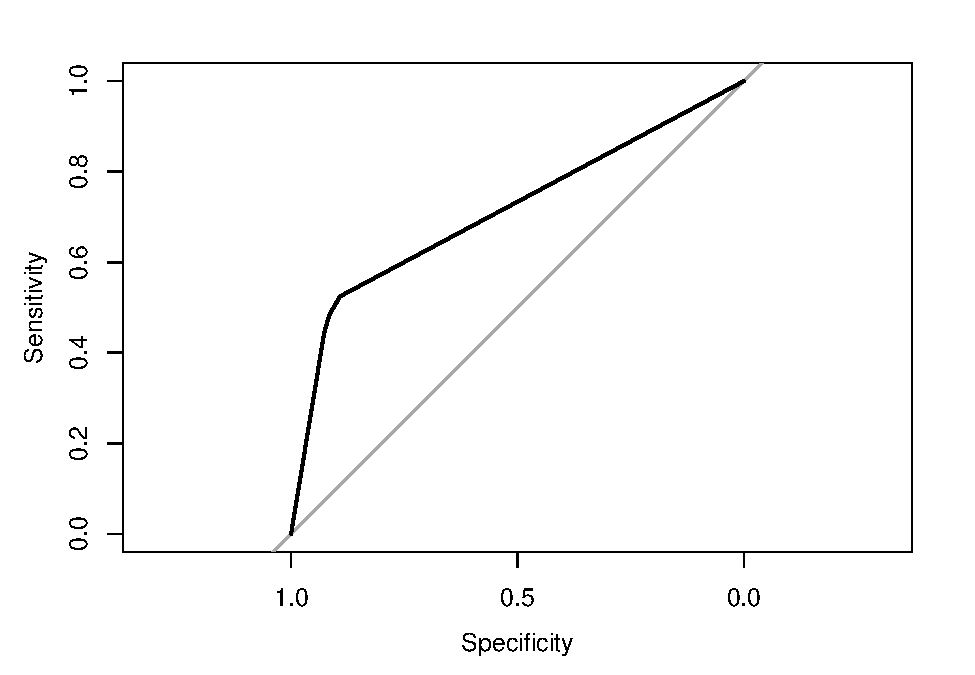
\includegraphics{02-logit_files/figure-latex/unnamed-chunk-19-1.pdf}

Mida suurem on pind graafiku kurvi all, seda parema mudeliga meil tegemist on (seda täpsemini võimaldab mudel prognoosida). Seda kurvi alust pindala suurust kasutataksegi prognoosi täpsuse hindamiseks. Vastavat statistikut kutsustaksegi kurvialuseks pindalaks (AUC ehk \emph{area under the curve}). Mida lähemal AUC \(1\)'le on, seda parema prognoosivõimega mudeliga meil tegemist on.

\begin{Shaded}
\begin{Highlighting}[]
\FunctionTok{auc}\NormalTok{(roc\_g)}
\end{Highlighting}
\end{Shaded}

\begin{verbatim}
## Area under the curve: 0.7133
\end{verbatim}

\hypertarget{poissoni-regressioon}{%
\chapter{Poissoni regressioon}\label{poissoni-regressioon}}

Poissoni regressioon kuulub üldistatud lineaarsete mudelite (GLM) raamistikku ja sellega saame hinnata sõltumatute tunnuste mõju mingile loendavale (\emph{count}) sõltuvale tunnusele (mitu inimest on kursusel, mitu inimest on poejärjekorras, mitu last on peres jne)\footnote{Ka kategoriaalsetest tunnustest moodustatud risttabelite sagedused on loendilised väärtused. Taoliste risttabelite sageduste baasil moodustatud mudeleid kutsutakse log-lineaarseteks mudeliteks. Lisaks loenditele kasutatakse Poissoni regressiooni ka määrade (\emph{rates}) mudeldamiseks, kuna määrasid võib käsitleda kui standardiseeritud loendeid. Siinkohal me taolisi mudeleid lähemalt ei käsitle, aga olgu see lihtsalt ära mainitud.}.

Sarnaselt logistilise regressiooniga (ja isegi õigustatumalt) tekib küsimus, et miks me ei saa taoliste tunnuste korral kasutada tavalist lineaarset regressiooni? Loend on ju suhteliselt sarnane tavalisele arvtunnusele. Välja arvatud asjaolu, et nii nagu tõenäosus logistilise regressiooni puhul, ei saa ka loend olla negatiivne. Kui me modelleeriksime loendi tunnust tavalise lineaarse regressiooniga, siis võib vabalt juhtuda, et mingite sõltumatute tunnuste väärtuste korral oleks prognoositav sõltuv tunnus väiksem kui 0. See aga ei ole loendilise tunnuse puhul realistlik. Lisaks, nii nagu ka logistilise regressiooni ja binaarsete sõltuvate tunnuste puhul, tekivad probleemid jääkide struktuuriga (tavaline regressioon eeldab normaaljaotust) ja jääkide dispersiooniga (tavaline regressioon eeldab konstantset hajuvust)\footnote{Loendiline tunnus \(Y\) järgib Poissoni jaotust, mille puhul \(E(Y)=Var(Y)=\lambda\), kus \(\lambda\) on nn keskmine loend (keskmine kursuse suurus, järjekorra pikkus, laste arv). Seega Poissoni jaotusega tunnuse puhul peaks keskmine ja dispersioon võrdsed olema ning suurem keskmine tähendab ka suuremat dispersioon.}.

\begin{figure}
\centering
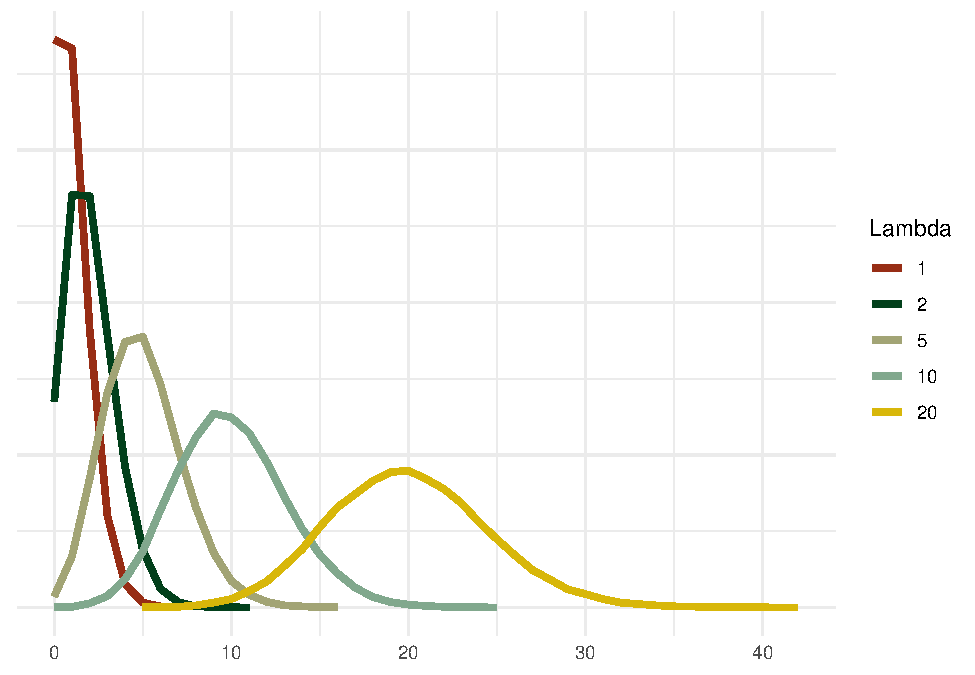
\includegraphics{03-poisson_files/figure-latex/pois-dist-1.pdf}
\caption{\label{fig:pois-dist}Poissoni jaotus erinevate keskmiste loendusväärtuste (Lambda) korral}
\end{figure}

Logistilise regressiooni puhul saime tõenäosuse ülemisest piirist lahti seeläbi, et teisendasime tõenäosused šanssideks ning alumise piiri seeläbi, et võtsime šanssidest logaritmid. Loendilise tunnuse puhul meil tunnuse ülemise piiriga probleemi ei ole. Loend võib potentsiaalselt olla lõputu. Alumise piiri puhul saame aga kasutada sedasama logit mudelitest tuttavat logaritmimise nippi. Kui \(Y\) on meie hinnatav loendiline sõltuv tunnus ja \(x\) seda selgitav sõltumatu tunnus, siis Poissoni regressioonimudel on väljendatav järgmiselt\footnote{\(log(Y_i)\) ei ole siin sama mis lineaarse regressiooni puhul log-transformeeritud tunnus (kui me kasutame analüüsis eelnevalt logaritmitud sõltuvat tunnust). Teine ja sellest aspektist võib-olla selgem notatsioon oleks \(log(E(Y))=\beta_0+\beta_1 x_i\), millest nähtub, et me peame logaritmima \(Y\) oodatavat väärtust (\emph{expected value}) ehk \(Y\) keskmist. Keskmine logaritmitud \(Y\) ja logaritm keskmisest \(Y\)-ist ei ole aga samad asjad (võite järgi proovida: \texttt{mean(log(c(1,2,3,4)))} vs \texttt{log(mean(c(1,2,3,4)))}).}:

\[log(Y_i)=\beta_0+\beta_1 x_i\]
kui me võtame mõlemast võrrandi pooles eksponendi, saame sama asja väljendada ka nii:

\[Y_i = e^{\beta_0+\beta_1 x_i}\]

Eeldame siin, et \(Y_i\) järgib Poissoni jaotust. GLM'i sõnavara kasutades ütleme, et mudeli juhuslik komponent (ehk siis sõltuv tunnus) on Poissoni jaotusega ning linkfunktsioonina (funktsiooon, mille abil sõltuva ja sõltumatute tunnuste vaheline mittelineaarne seos muudetakse lineaarseks seoseks) kasutame log-funktsiooni.

Poissoni jaotuse kuju sõltub tunnuse keskmisest (võrdluseks, normaaljaotuse kuju sõltub tunnuse keskmisest ja standardhälbest). Mida suurem on keskmine, seda enam sarnaneb Poissoni jaotus normaaljaotusele (vt joonis 1). Seega suurte loendite puhul saaksime põhimõtteliselt ka tavalist lineaarset regressiooni kasutada (kuigi negatiivsete väärtuste probleem jääb ka sel juhul). Üldiselt on mõistlik Poissoni regressiooni kasutada siis, kui loendite maksimaalsed väärtused ei ole väga suured ja tunnus on eripäraselt Poissoni jaotuse kujuga. Kui meil on tegemist suuremate väärtustega loendiga (näiteks ülikoolide tudengite arvud), siis saame tunnuse näiteks mingi arvuga läbi jagada.

Loendilise tunnuse puhul tuleb tihti ette olukordi, kus tunnuses on palju nulle. Näiteks tunnus, mis kirjeldab bakalaureusetudengite laste arvu. Põhimõtteliselt on muidugi tegemist loendilise tunnusega, aga kuna suuremal osal tudengitest veel ei ole lapsi, siis enamik vaatlusi on paratamatult nullid. Sellise tunnuse jaotus ei vasta väga hästi Poissoni jaotusele ja selle kasutamine Poissoni regressioonimudeliga ei anna tõenäoliselt väga head tulemust\footnote{Paljude nullidega tunnuse puhul oleks mõistlikum kasutada näiteks \emph{zero-inflated Poisson}'i regressiooni (\texttt{zeroinfl()} funktsioon \emph{pscl} paketis) või \emph{negative binomial} regressiooni (\texttt{glm.nb()} funktsioon \emph{MASS} paketis)}.

\hypertarget{mudeli-tuxf5lgendus-1}{%
\section{Mudeli tõlgendus}\label{mudeli-tuxf5lgendus-1}}

Kuidas me neid regressioonimudeli \(\beta_0\) ja \(\beta_1\) koefitsiente tõlgendama peaksime? Lineaarse regressiooni puhul oli asi lihtne: vabaliige (\(\beta_0\)) oli tõlgendatav \(Y\) väärtusena kui \(x\) on \(0\) ja regressioonikoefitsient (\(\beta_1\)) näitas \(Y\) muutust kui \(x\) muutub ühe ühiku võrra. Logistilise regressiooni puhul pidime aga esmalt koefitsientidest eksponendi võtma ja saime neid seejärel tõlgendada šansside ja šansside suhetena. Mis siis sekord?

Kuna meil on jälle tegemist logaritmidega, siis koefitsientide otsene (lineaarse regressiooni moodi) tõlgendamine on keeruline. Mõistlikum on koefitsientidest jällegi eksponent võtta, misjärel saame vabaliiget tõlgendada tavapärasel moel (\(Y\) väärtus kui \(x\) on \(0\)) ja regressioonikoefitsienti kui \(Y\)-i multiplikatiivset muutust kui \(x\) muutub ühe ühiku võrra. Ehk kui \(\beta_1\) väärtus on näiteks 0.25, siis tema eksponent on \(e^{0.25} = exp(0.25) = 1.28\) ja saame järeldada, et kui \(x\) kasvab ühe ühiku võrra, siis \(Y\) kasvab \(1.28\) korda. Teisisõnu, \(Y\) kasvab \(28\%\). Või kui \(\beta_1\) väärtus on \(-0.5\), siis tema eksponent on \(e^{-0.5} = exp(-0.5) = 0.6\) ja saame järeldada, et kui \(x\) kasvab ühe ühiku võrra, siis \(Y\) kasvab \(0.6\) korda (ehk siis tegelikult kahaneb). Kui \(\beta = 0\), siis \(e^{0} = 1\) ehk multiplikatiivne efekt on \(1\) (\(Y\times1\)) ja \(Y\) \(x\)-i kasvades või kahanedes ei muutu. Kui \(\beta < 0\), siis \(Y\) \(x\)-i kasvades väheneb, kui \(\beta > 0\), siis \(Y\) \(x\)-i kasvades kasvab.

\hypertarget{poissoni-regressiooni-eeldused}{%
\section{Poissoni regressiooni eeldused}\label{poissoni-regressiooni-eeldused}}

\begin{itemize}
\tightlist
\item
  Sõltuv tunnus \(Y\) peaks enam-vähem vastama Poissoni jaotusele (st olema loendiline tunnus).
\item
  Vaatlused peavad olema üksteisest sõltumatud (st kogu vaatluste vaheline seos peaks olema kirjeldatud mudeli sõltumatute tunnuste poolt).
\item
  Dispersioon (\emph{variance}) peaks olema võrdne keskmisega. Juhul kui see eeldus ei ole täidetud, ja tihti juhtub, et ei ole, on meil tegemist nn üledispersiooniga (\emph{overdispersion}). Sellisel juhul tuleks Poissoni mudeli asemel kasutada nn \emph{quasipoisson}'i mudelit.
\item
  Sõltuva tunnuse ja sõltumatute prediktorite seos peaks läbi linkfunktsiooni olema lineaarne.
\end{itemize}

\hypertarget{mudeli-hindamine-r-is}{%
\section{Mudeli hindamine R-is}\label{mudeli-hindamine-r-is}}

\hypertarget{andmete-kirjeldus-ja-ettevalmistus}{%
\subsection{Andmete kirjeldus ja ettevalmistus}\label{andmete-kirjeldus-ja-ettevalmistus}}

Kasutame näitena \emph{PhDPublications} andmestikku\footnote{Long, J.S. (1997). The Origin of Sex Differences in Science. Social Forces, 68, 1297--1315.} paketist \emph{AER}. Andmestikus on loendatud biokeemia doktorantide publikatsioonide arv (tunnus \emph{atricles}) kolme aasta jooksul. Sõltumatute tunnustena on kasutada:

\begin{itemize}
\tightlist
\item
  \emph{gender},
\item
  \emph{married} - kas doktorant oli abielus,
\item
  \emph{kids} - mitu last doktorandil oli,
\item
  \emph{prestige} - kooli maine skoor) ja
\item
  \emph{mentor} - juhendaja publikatsioonide arv.
\end{itemize}

\begin{Shaded}
\begin{Highlighting}[]
\CommentTok{\# Kui pakett ei ole installitud, }
\CommentTok{\# tuleb seda teha käsuga: install.packages("AER")}

\CommentTok{\# Loeme paketi sisse}
\FunctionTok{library}\NormalTok{(AER)}
\CommentTok{\# Võtame andmestiku}
\FunctionTok{data}\NormalTok{(PhDPublications)}
\CommentTok{\# Paneme andmestikule lihtsama nime}
\NormalTok{phd }\OtherTok{\textless{}{-}}\NormalTok{ PhDPublications}
\end{Highlighting}
\end{Shaded}

Vaatame artiklite tunnust lähemalt:

\begin{Shaded}
\begin{Highlighting}[]
\FunctionTok{ggplot}\NormalTok{(phd)}\SpecialCharTok{+}
  \FunctionTok{geom\_histogram}\NormalTok{(}\FunctionTok{aes}\NormalTok{(}\AttributeTok{x =}\NormalTok{ articles), }
                 \AttributeTok{binwidth =} \DecValTok{1}\NormalTok{, }
                 \AttributeTok{fill =} \StringTok{\textquotesingle{}grey\textquotesingle{}}\NormalTok{, }
                 \AttributeTok{color =} \StringTok{\textquotesingle{}black\textquotesingle{}}\NormalTok{)}\SpecialCharTok{+}
  \FunctionTok{theme\_minimal}\NormalTok{()}
\end{Highlighting}
\end{Shaded}

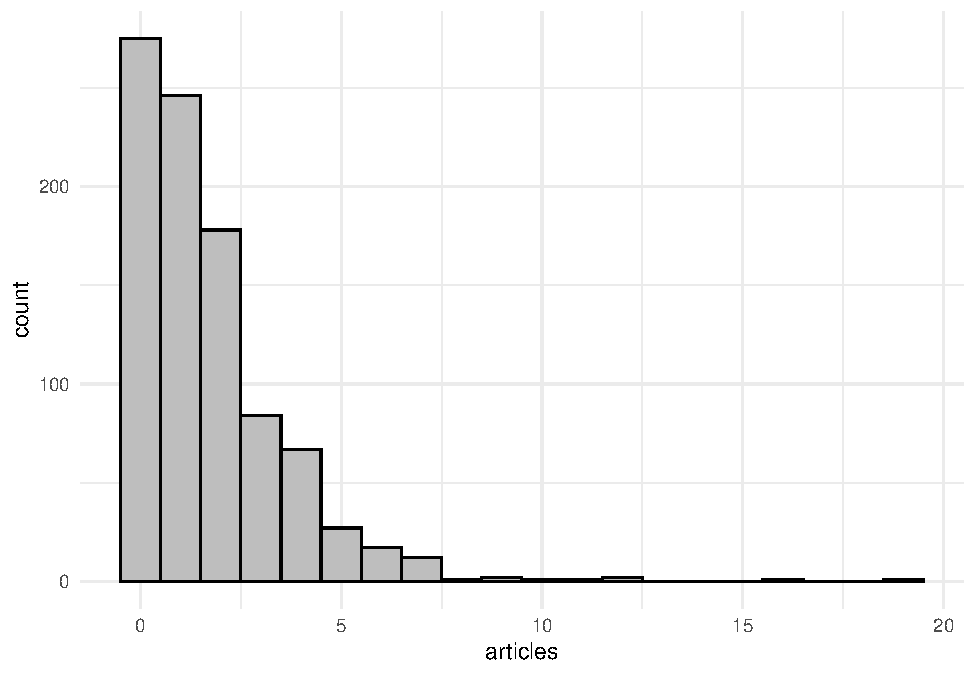
\includegraphics{03-poisson_files/figure-latex/unnamed-chunk-2-1.pdf}

Ilmselgelt on tegemist loendilise tunnusega. Samas päris Poissoni jaotusega tegemist vist siiski ei ole, kuna tundub, et nulle on selleks natukene liiga palju. ggploti abil saame joonisele panna ka tunnust iseloomustava teoreetilise Poissoni jaotuse (lähtuvalt tunnuse keskmisest ehk \(\lambda\) parameetrist). Vaatame kuidas see võrreldes reaalse jaotusega välja näeb:

\begin{Shaded}
\begin{Highlighting}[]
\CommentTok{\# Poissoni jaotuse parameetrina on meil vaja keskmist}
\NormalTok{keskmine }\OtherTok{\textless{}{-}} \FunctionTok{mean}\NormalTok{(phd}\SpecialCharTok{$}\NormalTok{articles)}
\NormalTok{phd }\SpecialCharTok{\%\textgreater{}\%} 
  \CommentTok{\# standardiseerime  artiklite arvu, }
  \CommentTok{\# et saaksime seda jaotusega võrrelda}
  \FunctionTok{group\_by}\NormalTok{(articles) }\SpecialCharTok{\%\textgreater{}\%} 
  \FunctionTok{summarise}\NormalTok{(}\AttributeTok{n =} \FunctionTok{n}\NormalTok{()) }\SpecialCharTok{\%\textgreater{}\%} 
  \FunctionTok{mutate}\NormalTok{(}\AttributeTok{n\_scaled =}\NormalTok{ n}\SpecialCharTok{/}\FunctionTok{sum}\NormalTok{(n)) }\SpecialCharTok{\%\textgreater{}\%} 
\FunctionTok{ggplot}\NormalTok{(}\FunctionTok{aes}\NormalTok{(}\AttributeTok{x =}\NormalTok{ articles, }\AttributeTok{y =}\NormalTok{ n\_scaled))}\SpecialCharTok{+}
  \CommentTok{\# kasutame stat = \textquotesingle{}identity\textquotesingle{}, }
  \CommentTok{\# st kasutame joonisel olemasolevaid väärtusi}
  \CommentTok{\# (mitte ei lase ggplot\textquotesingle{}il neid välja arvutada)}
  \FunctionTok{geom\_histogram}\NormalTok{(}\AttributeTok{stat =} \StringTok{\textquotesingle{}identity\textquotesingle{}}\NormalTok{, }
                 \AttributeTok{fill =} \StringTok{\textquotesingle{}grey\textquotesingle{}}\NormalTok{, }
                 \AttributeTok{color =} \StringTok{\textquotesingle{}black\textquotesingle{}}\NormalTok{)}\SpecialCharTok{+}
  \CommentTok{\# dpois funktsioon annab meile poissoni tihedusfunktsiooni}
  \FunctionTok{geom\_line}\NormalTok{(}\FunctionTok{aes}\NormalTok{(}\AttributeTok{x =}\NormalTok{ articles, }
                \AttributeTok{y =} \FunctionTok{dpois}\NormalTok{(articles, }\AttributeTok{lambda =}\NormalTok{ keskmine)), }
            \AttributeTok{color =} \StringTok{\textquotesingle{}red\textquotesingle{}}\NormalTok{)}\SpecialCharTok{+}
  \FunctionTok{theme\_minimal}\NormalTok{()}
\end{Highlighting}
\end{Shaded}

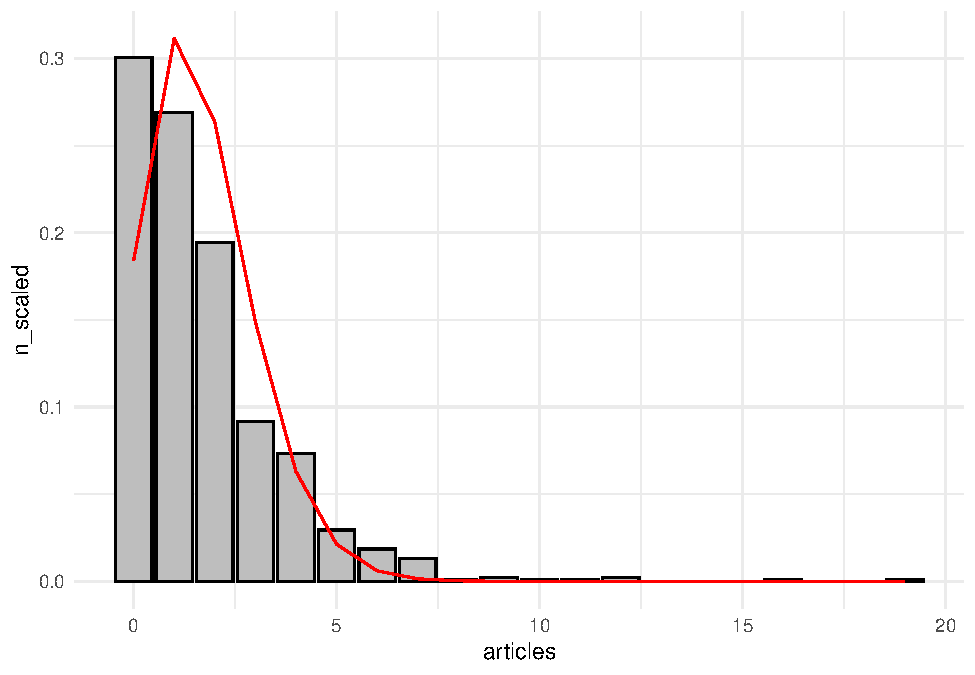
\includegraphics{03-poisson_files/figure-latex/pois-hist-dist-1.pdf}

Nagu näeme, siis tõesti, nulle on natuke liiga palju ja artiklite loendi jaotus ei vasta jaotuse alguses päris täpselt Poissoni jaotuse kujule. Aga jätame selle asjaolu hetkel tähelepanuta ja kasutame ikkagi Poissoni regressiooni.

Vaatame üle ka teised andmestiku tunnused:

\begin{Shaded}
\begin{Highlighting}[]
\NormalTok{phd }\SpecialCharTok{\%\textgreater{}\%} 
  \FunctionTok{group\_by}\NormalTok{(gender) }\SpecialCharTok{\%\textgreater{}\%} 
  \FunctionTok{summarize}\NormalTok{(}\FunctionTok{n}\NormalTok{())}
\end{Highlighting}
\end{Shaded}

\begin{verbatim}
## # A tibble: 2 x 2
##   gender `n()`
##   <fct>  <int>
## 1 male     494
## 2 female   421
\end{verbatim}

\begin{Shaded}
\begin{Highlighting}[]
\NormalTok{phd }\SpecialCharTok{\%\textgreater{}\%} 
  \FunctionTok{group\_by}\NormalTok{(married) }\SpecialCharTok{\%\textgreater{}\%} 
  \FunctionTok{summarize}\NormalTok{(}\FunctionTok{n}\NormalTok{())}
\end{Highlighting}
\end{Shaded}

\begin{verbatim}
## # A tibble: 2 x 2
##   married `n()`
##   <fct>   <int>
## 1 no        309
## 2 yes       606
\end{verbatim}

Soo ja abielu tunnus tunduvad korras olevat, kui välja arvata see, et kuidagi paljud doktorandid paistavad abielus olevat. Aga on nagu on.

\begin{Shaded}
\begin{Highlighting}[]
\NormalTok{phd }\SpecialCharTok{\%\textgreater{}\%} 
  \FunctionTok{group\_by}\NormalTok{(kids) }\SpecialCharTok{\%\textgreater{}\%} 
  \FunctionTok{summarize}\NormalTok{(}\FunctionTok{n}\NormalTok{())}
\end{Highlighting}
\end{Shaded}

\begin{verbatim}
## # A tibble: 4 x 2
##    kids `n()`
##   <int> <int>
## 1     0   599
## 2     1   195
## 3     2   105
## 4     3    16
\end{verbatim}

Laste tunnus on originaalis arvuline. Me kindlasti ei taha nelja väärtusega tunnust arvulisena käsitleda. Parem oleks see faktoriks teha ja seda mudelis kategoriaalsena käsitleda. Antud juhul, kuna lastetuid doktorante on niivõrd palju, oleks vast kõige mõistlik see tunnus üldse binaarseks teha, st kas on või ei ole lapsi (kuigi teoreetiliselt võiks ju eeldada, et laste arv võib mõjutada artiklite kirjutamiseks jäävat aega, siis siin, mulle tundub, on laste arvu variatiivsus selle kasutamiseks liiga väike).

\begin{Shaded}
\begin{Highlighting}[]
\CommentTok{\# kasutame laste arvu teisendamiseks ifelse() funktsiooni}
\CommentTok{\# vajadusel vaadake sellekohast abiinfot ?ifelse}
\NormalTok{phd }\OtherTok{\textless{}{-}}\NormalTok{ phd }\SpecialCharTok{\%\textgreater{}\%} 
  \FunctionTok{mutate}\NormalTok{(}\AttributeTok{kids2 =} \FunctionTok{ifelse}\NormalTok{(kids }\SpecialCharTok{==} \DecValTok{0}\NormalTok{, }\StringTok{\textquotesingle{}Ei\textquotesingle{}}\NormalTok{, }\StringTok{\textquotesingle{}Jah\textquotesingle{}}\NormalTok{))}

\CommentTok{\# kontrollime uut tunnust}
\NormalTok{phd }\SpecialCharTok{\%\textgreater{}\%} 
  \FunctionTok{group\_by}\NormalTok{(kids, kids2) }\SpecialCharTok{\%\textgreater{}\%} 
  \FunctionTok{summarise}\NormalTok{(}\FunctionTok{n}\NormalTok{())}
\end{Highlighting}
\end{Shaded}

\begin{verbatim}
## # A tibble: 4 x 3
## # Groups:   kids [4]
##    kids kids2 `n()`
##   <int> <chr> <int>
## 1     0 Ei      599
## 2     1 Jah     195
## 3     2 Jah     105
## 4     3 Jah      16
\end{verbatim}

Pidevast tunnusest ülevaate saamiseks on mugav kasutada histogrammi:

\begin{Shaded}
\begin{Highlighting}[]
\FunctionTok{hist}\NormalTok{(phd}\SpecialCharTok{$}\NormalTok{prestige)}
\end{Highlighting}
\end{Shaded}

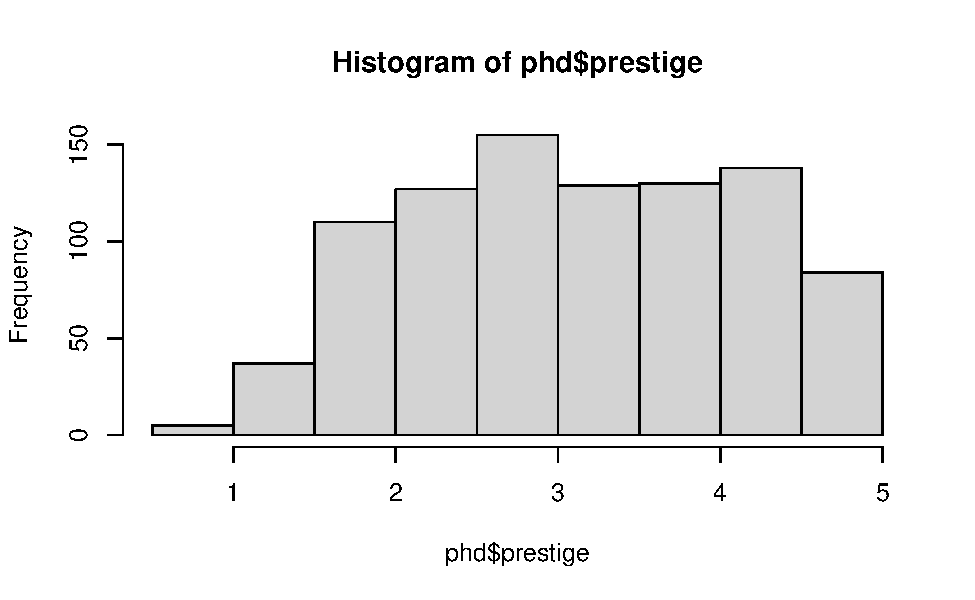
\includegraphics{03-poisson_files/figure-latex/unnamed-chunk-7-1.pdf}

PhD programmi maine küsimus tundub suht OK.

\begin{Shaded}
\begin{Highlighting}[]
\FunctionTok{hist}\NormalTok{(phd}\SpecialCharTok{$}\NormalTok{mentor)}
\end{Highlighting}
\end{Shaded}

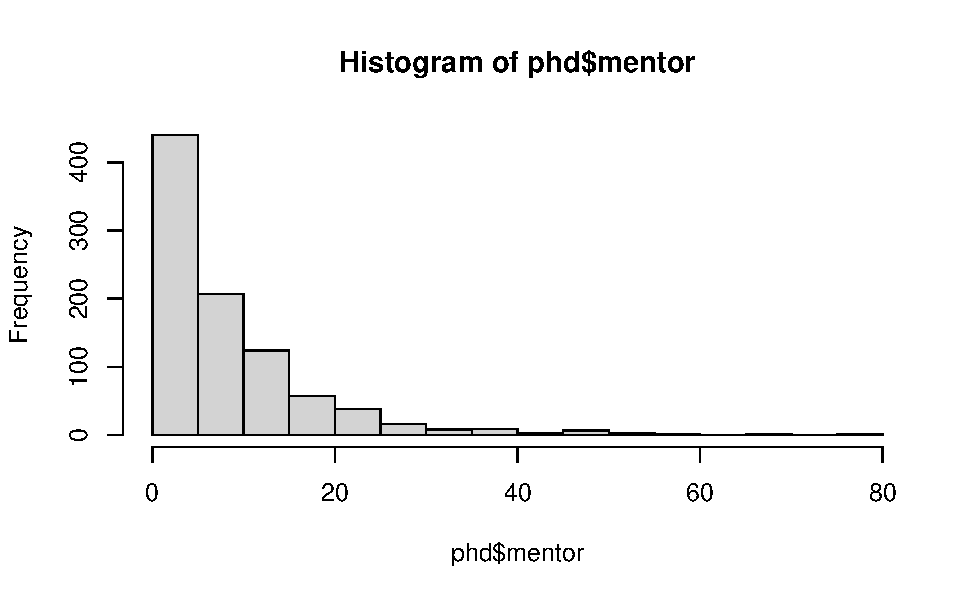
\includegraphics{03-poisson_files/figure-latex/unnamed-chunk-8-1.pdf}

Juhendaja artiklit arvu tunnus on iseenesest samuti loendav tunnus (kuigi Poissoni jaotust see samuti päris täpselt ei järgi).

\hypertarget{poissoni-mudeli-defineerimine}{%
\subsection{Poissoni mudeli defineerimine}\label{poissoni-mudeli-defineerimine}}

Vaatame esmalt kuidas sugu artiklite avaldamist mõjutab. Defineerime mudeli kasutades \texttt{glm()} funktsiooni ja selles \texttt{family\ =} argumendina \texttt{poisson()} funktsiooni (kõlbaks ka \texttt{family\ =\ "poisson"} või \texttt{family\ =\ poisson}). \texttt{poisson()} funktsiooni puhul on vaikimisi eeldatud linkfunktsioonina \texttt{log}-linki, kuid vajadusel saaksime ka mingit muud linkfunktsiooni kasutada või selle eksplitsiitselt välja tuua: \texttt{poisson(link\ =\ \textquotesingle{}log\textquotesingle{})}. Salvestame mudeli kõigepealt andmeobjektiks ning seejärel uurime seda \texttt{summary()} funktsiooniga.

\begin{Shaded}
\begin{Highlighting}[]
\NormalTok{m1 }\OtherTok{\textless{}{-}} \FunctionTok{glm}\NormalTok{(articles}\SpecialCharTok{\textasciitilde{}}\NormalTok{gender, }\AttributeTok{family =} \FunctionTok{poisson}\NormalTok{(), }\AttributeTok{data =}\NormalTok{ phd)}
\FunctionTok{summary}\NormalTok{(m1)}
\end{Highlighting}
\end{Shaded}

\begin{verbatim}
## 
## Call:
## glm(formula = articles ~ gender, family = poisson(), data = phd)
## 
## Deviance Residuals: 
##     Min       1Q   Median       3Q      Max  
## -1.9404  -1.7148  -0.4119   0.4139   7.3221  
## 
## Coefficients:
##              Estimate Std. Error z value Pr(>|z|)    
## (Intercept)   0.63265    0.03279  19.293  < 2e-16 ***
## genderfemale -0.24718    0.05187  -4.765 1.89e-06 ***
## ---
## Signif. codes:  0 '***' 0.001 '**' 0.01 '*' 0.05 '.' 0.1 ' ' 1
## 
## (Dispersion parameter for poisson family taken to be 1)
## 
##     Null deviance: 1817.4  on 914  degrees of freedom
## Residual deviance: 1794.4  on 913  degrees of freedom
## AIC: 3466.1
## 
## Number of Fisher Scoring iterations: 5
\end{verbatim}

Nagu näeme, siis Poissoni regressiooni väljund on praktiliselt identne logistilise regressiooni väljundiga (mis on ka loogiline, kuna mõlemad on loodud sama funktsiooniga).

Tõlgendame kõigepealt regressioonikoefitsiente. Nagu eelnevalt mainitud, siis tuleks neist eelnevalt eksponent võtta. Aga ka ilma selleta saame öelda, et naised on meestest vähem artikleid avaldanud. Mehed on antud juhul referentsgrupp ning \emph{genderfemale} koefitsient kirjeldab naiste erinevust meestest. Kuna koefitsient on negatiivne, siis saame järeldada, et keskmine artiklite arv on naiste hulgas väiksem kui meeste hulgas. Aga et teada saada kui palju väiksem, peame koefitsientidest eksponendi võtma:

\begin{Shaded}
\begin{Highlighting}[]
\CommentTok{\# koefitsiendid saame mudeli objektist kätte coef() funktsiooniga}
\FunctionTok{exp}\NormalTok{(}\FunctionTok{coef}\NormalTok{(m1))}
\end{Highlighting}
\end{Shaded}

\begin{verbatim}
##  (Intercept) genderfemale 
##    1.8825911    0.7810027
\end{verbatim}

Vabaliige on \(Y\) väärtus kui \(x\) on \(0\). Kuna mehed on referentsgrupp (ehk siis \(0\)), siis kirjeldab vabaliige siinkohal meeste keskmist artiklite arvu. Võime tulemuse \texttt{dplyr}'iga verifitseerida:

\begin{Shaded}
\begin{Highlighting}[]
\NormalTok{phd }\SpecialCharTok{\%\textgreater{}\%} 
  \FunctionTok{filter}\NormalTok{(gender }\SpecialCharTok{==} \StringTok{\textquotesingle{}male\textquotesingle{}}\NormalTok{) }\SpecialCharTok{\%\textgreater{}\%} 
  \FunctionTok{summarize}\NormalTok{(}\FunctionTok{mean}\NormalTok{(articles))}
\end{Highlighting}
\end{Shaded}

\begin{verbatim}
##   mean(articles)
## 1       1.882591
\end{verbatim}

Tundub tõesti nii olevat.

Eksponenti võetud \emph{genderfemale} koefitsient näitab naiste multiplikatiivset erinevust meestest. Ehk siis naiste keskmine artiklite arv peaks olema \(1.88 \times 0.78 = 1.47\). Teiste sõnadega naiste keskmine artiklite arv on \(1-0.78 = 22\%\) väiksem kui meestel. Kontrollime üle:

\begin{Shaded}
\begin{Highlighting}[]
\NormalTok{phd }\SpecialCharTok{\%\textgreater{}\%} 
  \FunctionTok{filter}\NormalTok{(gender }\SpecialCharTok{==} \StringTok{\textquotesingle{}female\textquotesingle{}}\NormalTok{) }\SpecialCharTok{\%\textgreater{}\%} 
  \FunctionTok{summarize}\NormalTok{(}\FunctionTok{mean}\NormalTok{(articles))}
\end{Highlighting}
\end{Shaded}

\begin{verbatim}
##   mean(articles)
## 1       1.470309
\end{verbatim}

Jälle sama tulemus.

Mida me veel tulemist näeme ja näha tahame? Eelkõige huvitab meid muidugi see, kas meie tulemused on statistiliselt usaldusväärsed. Regressioonikordajate statistilise olulisuse hindamiseks on meil analoogselt logistilise regressiooni väljundiga kasutada z-test, mis testib kas regressioonikordaja on oluliselt erinev nullist. Näeme nii teststatistikut (z-väärtust), kui ka z-testi iseloomustavat \emph{p}-väärtust. \emph{p} väärtused (tulp \texttt{Pr(\textgreater{}\textbar{}z\textbar{})}) on nii vabaliikme kui regressioonikoefitsiendi puhul oluliselt väiksemad kui \(0.05\), misläbi saame järeldada, et usaldusnivool \(95\%\) on meie mudeli koefitsiendid statistiliselt oluliselt erinevad nullist\footnote{\emph{p}-väärtus ütleb meile, et juhul kui nullhüpotees oleks tõsi (antud juhul on nullhüpoteesiks, et tunnuste vahel ei ole seost, st regressioonikoefitsient on \(0\)), siis saaksime sellise tulemuse nagu me saime (täpsemalt öeldes sellise z-väärtuse) tõenäosusega mis on võrdne \emph{p}-väärtusega. Kui \emph{p}-väärtus on näiteks \(0.05\), siis uuringut korrates saaksime sellise tulemuse \(5\%\) kordadest. Antud juhul on \emph{p}-väärtus oluliselt väiksem kui \(0.5\), st tõenäosus, et meie regressioonikordaja on tegelikult \(0\), on hästi väike.}, ehk siis sugu mõjutab oluliselt avaldatud artiklite arvu. Kui koefitsient ei oleks statistiliselt oluline (\(p > 0.05\)), siis peaksime järeldama, et meie koefitsient ei erine oluliselt nullist ning seost sõltumatu ja sõltuva tunnuse vahel ei ole.

Sama järelduse saaksime tegelikult teha ka z-väärtuste ja standardvigade (tulp \texttt{Std.\ Error}) põhjal. Mida väiksem on z-väärtus, seda väiksem on \emph{p}. Ja kui z-väärtus on (absoluutarvuna) suurem kui \(1.96\), siis on \emph{p} on väiksem kui \(0.05\). Ning z-väärtus (ja z-test) omakorda tuleneb standardveast: \(\frac{-0.24718}{0.05187} = -4.765\).

Aga vaatame oma mudelit edasi. Lisame ka teised sõltumatud tunnused:

\begin{Shaded}
\begin{Highlighting}[]
\NormalTok{m2 }\OtherTok{\textless{}{-}} \FunctionTok{glm}\NormalTok{(articles}\SpecialCharTok{\textasciitilde{}}\NormalTok{gender}\SpecialCharTok{+}\NormalTok{prestige}\SpecialCharTok{+}\NormalTok{married}\SpecialCharTok{+}\NormalTok{kids2}\SpecialCharTok{+}\NormalTok{mentor, }\AttributeTok{family =} \FunctionTok{poisson}\NormalTok{(), }\AttributeTok{data =}\NormalTok{ phd)}
\FunctionTok{summary}\NormalTok{(m2)}
\end{Highlighting}
\end{Shaded}

\begin{verbatim}
## 
## Call:
## glm(formula = articles ~ gender + prestige + married + kids2 + 
##     mentor, family = poisson(), data = phd)
## 
## Deviance Residuals: 
##     Min       1Q   Median       3Q      Max  
## -3.4477  -1.5669  -0.3587   0.5705   5.4715  
## 
## Coefficients:
##               Estimate Std. Error z value Pr(>|z|)    
## (Intercept)   0.306243   0.103093   2.971  0.00297 ** 
## genderfemale -0.217925   0.054717  -3.983 6.81e-05 ***
## prestige      0.010275   0.026460   0.388  0.69776    
## marriedyes    0.151697   0.063028   2.407  0.01609 *  
## kids2Jah     -0.249563   0.063342  -3.940 8.15e-05 ***
## mentor        0.025817   0.002019  12.788  < 2e-16 ***
## ---
## Signif. codes:  0 '***' 0.001 '**' 0.01 '*' 0.05 '.' 0.1 ' ' 1
## 
## (Dispersion parameter for poisson family taken to be 1)
## 
##     Null deviance: 1817.4  on 914  degrees of freedom
## Residual deviance: 1640.9  on 909  degrees of freedom
## AIC: 3320.7
## 
## Number of Fisher Scoring iterations: 5
\end{verbatim}

Näeme, et ülikooli maine ei mõjuta statistiliselt oluliselt artiklite arvu. Ka abielustaatus on suhteliselt piiripealse mõjuga. Jätame maine tunnuse mudelist välja (tahame alati leida võimalikult lihtsa mudeli, seega tunnused, mis mudelisse ei ei panusta, jätame välja).

\begin{Shaded}
\begin{Highlighting}[]
\NormalTok{m3 }\OtherTok{\textless{}{-}} \FunctionTok{glm}\NormalTok{(articles}\SpecialCharTok{\textasciitilde{}}\NormalTok{gender}\SpecialCharTok{+}\NormalTok{married}\SpecialCharTok{+}\NormalTok{kids2}\SpecialCharTok{+}\NormalTok{mentor, }\AttributeTok{family =} \FunctionTok{poisson}\NormalTok{(), }\AttributeTok{data =}\NormalTok{ phd)}
\end{Highlighting}
\end{Shaded}

Kontrollime igaks juhuks ka \texttt{anova()}-ga, kas maine tunnuse väljajätmine ikka oli õigustatud:

\begin{Shaded}
\begin{Highlighting}[]
\FunctionTok{anova}\NormalTok{(m3, m2, }\AttributeTok{test =} \StringTok{\textquotesingle{}Chisq\textquotesingle{}}\NormalTok{)}
\end{Highlighting}
\end{Shaded}

\begin{verbatim}
## Analysis of Deviance Table
## 
## Model 1: articles ~ gender + married + kids2 + mentor
## Model 2: articles ~ gender + prestige + married + kids2 + mentor
##   Resid. Df Resid. Dev Df Deviance Pr(>Chi)
## 1       910     1641.1                     
## 2       909     1640.9  1  0.15093   0.6976
\end{verbatim}

Hii-ruut test ütleb meile, et keerulisema ja lihtsama mudeli vahel ei ole statistiliselt olulist erinevust (\(p > 0.05\)), seega võime tunnuse vabalt välja jätta.

Näeme, et nii sugu, abielustaatus, laste arv, kui ka juhendaja publikatsioonide arv mõjutavad artiklite arvu oluliselt. Kontrollime igaks juhuks ka soo ja laste olemasolu koosmõju:

\begin{Shaded}
\begin{Highlighting}[]
\NormalTok{m4 }\OtherTok{\textless{}{-}} \FunctionTok{glm}\NormalTok{(articles}\SpecialCharTok{\textasciitilde{}}\NormalTok{gender}\SpecialCharTok{*}\NormalTok{kids2}\SpecialCharTok{+}\NormalTok{married}\SpecialCharTok{+}\NormalTok{mentor, }\AttributeTok{family =} \FunctionTok{poisson}\NormalTok{(), }\AttributeTok{data =}\NormalTok{ phd)}
\FunctionTok{summary}\NormalTok{(m4)}
\end{Highlighting}
\end{Shaded}

\begin{verbatim}
## 
## Call:
## glm(formula = articles ~ gender * kids2 + married + mentor, family = poisson(), 
##     data = phd)
## 
## Deviance Residuals: 
##     Min       1Q   Median       3Q      Max  
## -3.4995  -1.5593  -0.3582   0.5639   5.4570  
## 
## Coefficients:
##                       Estimate Std. Error z value Pr(>|z|)    
## (Intercept)            0.34220    0.06249   5.476 4.35e-08 ***
## genderfemale          -0.22492    0.06299  -3.571 0.000356 ***
## kids2Jah              -0.25695    0.07148  -3.595 0.000325 ***
## marriedyes             0.14875    0.06291   2.365 0.018045 *  
## mentor                 0.02601    0.00196  13.268  < 2e-16 ***
## genderfemale:kids2Jah  0.02522    0.12539   0.201 0.840628    
## ---
## Signif. codes:  0 '***' 0.001 '**' 0.01 '*' 0.05 '.' 0.1 ' ' 1
## 
## (Dispersion parameter for poisson family taken to be 1)
## 
##     Null deviance: 1817.4  on 914  degrees of freedom
## Residual deviance: 1641.0  on 909  degrees of freedom
## AIC: 3320.8
## 
## Number of Fisher Scoring iterations: 5
\end{verbatim}

Koosmõju koefitsient ei ole statistiliselt oluline, seega jääme mudeli m3 juurde:

\begin{Shaded}
\begin{Highlighting}[]
\FunctionTok{summary}\NormalTok{(m3)}
\end{Highlighting}
\end{Shaded}

\begin{verbatim}
## 
## Call:
## glm(formula = articles ~ gender + married + kids2 + mentor, family = poisson(), 
##     data = phd)
## 
## Deviance Residuals: 
##     Min       1Q   Median       3Q      Max  
## -3.5080  -1.5615  -0.3626   0.5614   5.4494  
## 
## Coefficients:
##              Estimate Std. Error z value Pr(>|z|)    
## (Intercept)   0.33873    0.06011   5.635 1.75e-08 ***
## genderfemale -0.21864    0.05470  -3.997 6.42e-05 ***
## marriedyes    0.14953    0.06279   2.381   0.0172 *  
## kids2Jah     -0.25029    0.06332  -3.953 7.73e-05 ***
## mentor        0.02600    0.00196  13.268  < 2e-16 ***
## ---
## Signif. codes:  0 '***' 0.001 '**' 0.01 '*' 0.05 '.' 0.1 ' ' 1
## 
## (Dispersion parameter for poisson family taken to be 1)
## 
##     Null deviance: 1817.4  on 914  degrees of freedom
## Residual deviance: 1641.1  on 910  degrees of freedom
## AIC: 3318.8
## 
## Number of Fisher Scoring iterations: 5
\end{verbatim}

Järgmiseks võtame mudeli koefitsientide eksponendid, et neid natukene inimlikumal kujul kuvada ja tõlgendada:

\begin{Shaded}
\begin{Highlighting}[]
\FunctionTok{exp}\NormalTok{(}\FunctionTok{coef}\NormalTok{(m3))}
\end{Highlighting}
\end{Shaded}

\begin{verbatim}
##  (Intercept) genderfemale   marriedyes     kids2Jah       mentor 
##    1.4031677    0.8036087    1.1612850    0.7785778    1.0263406
\end{verbatim}

Mida need koefitsiendid meile ütlevad?

\begin{itemize}
\tightlist
\item
  Vabaliige on antud näite puhul artiklite arv juhul kui kõikide sõltumatute tunnuste väärtused on nullid (ehk siis kõik kategoorilised tunnused on referentsväärtusega ja pidevtunnused lihtsalt nullid). Konkreetsel juhul on see ka sisukas tulemus, kuna mudeli ainsa pidevtunnuse nullväärtus on täiesti realistilik (juhendaja artiklite arv võib vabalt \(0\) olla). Aga üldiselt see pigem nii ei ole (mida me hakkame peale \(Y\) väärtusega, mis kehtib olukorras kus vanus või kehakaal on \(0\)). Seega, meie mudeli järgi on vallaliste, ilma lasteta meeste, kelle juhendajad pole viimase kolme aasta jooksul ühtegi publikatsiooni avaldanud, artiklite arv keskmiselt 1.4.
\item
  Naiste keskmine publikatsioonide arv (hoides teisi tunnuseid konstantsetena) on keskmiselt 20\% väiksem (\(1-0.8 = 0.2 = 20\%\)) kui meestel.
\item
  Abielus doktorantide keskmine publikatsioonide arv on \(1.16\) ehk \(16\%\) suurem kui vallalistel doktorantidel.
\item
  Laste olemasolu pärsib artiklite avaldamist keskmiselt \(22\%\) võrra.
\item
  Iga juhendaja lisanduv artikkel tõstab juhendatava publitseerimisvõimekust \(2\%\) võrra.
\end{itemize}

\hypertarget{mudeli-eelduste-kontroll}{%
\section{Mudeli eelduste kontroll}\label{mudeli-eelduste-kontroll}}

\hypertarget{uxfcledispersioon}{%
\subsection{Üledispersioon}\label{uxfcledispersioon}}

Mudeli üledispersioon (\emph{overdispersion}) on olukord, kus mudeli dispersioon on suurem kui mudeli aluseks olev jaotusfunktsioon eeldaks. Kui see on nii, siis on mudeli standardvead tõenäoliselt liiga väikesed (ja seega mudeli alusel tehtavad järldused valed). Üledispersiooni olemasolu saame kontrollida võrreldes jääkhälbimust (\emph{Residual deviance}) ja selle vabadusastemid (\emph{degrees of freedom} ehk \emph{df}). Kui need on enam-vähem võrdsed, ehk \(\frac{\text{Residual deviance}}{\text{df}} \approx 1\), siis üledispersiooni ei ole. Aga kui see suhe on oluliselt suurem kui \(1\), siis on tegemist probleemiga. Juhul kui taoline olukord esineb, peaksime Poissoni mudeli asemel kasutama \emph{quasipoisson}'i mudelit, kus üledispersiooni on eraldi dispersiooni parameetrina mudelis arvesse võetud. Ka meie näite puhul on tegemist kerge üledispersiooniga (mitte küll väga suurega, aga siiski), seega võiksime kasutada quasipoissonit:

\begin{Shaded}
\begin{Highlighting}[]
\NormalTok{m5 }\OtherTok{\textless{}{-}} \FunctionTok{glm}\NormalTok{(articles}\SpecialCharTok{\textasciitilde{}}\NormalTok{gender}\SpecialCharTok{+}\NormalTok{married}\SpecialCharTok{+}\NormalTok{kids2}\SpecialCharTok{+}\NormalTok{mentor, }\AttributeTok{family =}\NormalTok{ quasipoisson, }\AttributeTok{data =}\NormalTok{ phd)}
\FunctionTok{summary}\NormalTok{(m5)}
\end{Highlighting}
\end{Shaded}

\begin{verbatim}
## 
## Call:
## glm(formula = articles ~ gender + married + kids2 + mentor, family = quasipoisson, 
##     data = phd)
## 
## Deviance Residuals: 
##     Min       1Q   Median       3Q      Max  
## -3.5080  -1.5615  -0.3626   0.5614   5.4494  
## 
## Coefficients:
##               Estimate Std. Error t value Pr(>|t|)    
## (Intercept)   0.338732   0.081482   4.157 3.53e-05 ***
## genderfemale -0.218643   0.074151  -2.949  0.00327 ** 
## marriedyes    0.149527   0.085110   1.757  0.07928 .  
## kids2Jah     -0.250286   0.085834  -2.916  0.00363 ** 
## mentor        0.026000   0.002656   9.788  < 2e-16 ***
## ---
## Signif. codes:  0 '***' 0.001 '**' 0.01 '*' 0.05 '.' 0.1 ' ' 1
## 
## (Dispersion parameter for quasipoisson family taken to be 1.837376)
## 
##     Null deviance: 1817.4  on 914  degrees of freedom
## Residual deviance: 1641.1  on 910  degrees of freedom
## AIC: NA
## 
## Number of Fisher Scoring iterations: 5
\end{verbatim}

Näeme, et punkthinnangud ei muutunud, küll aga läksid standardvead suuremaks. See tähendab, et quaipoissoniga meie mudeli täpsusaste kahaneb (või õigemini esialgse, tavalise Poissoni mudeli puhul hindasime me mudeli täpsust üle). Samuti näeme, et tänu sellele ei ole abielustaatuse koefitsient enam \(95\%\) usaldusnivoo korral statistiliselt oluline ja peaksime selle tunnuse välja jätma.

\begin{Shaded}
\begin{Highlighting}[]
\NormalTok{m6 }\OtherTok{\textless{}{-}} \FunctionTok{glm}\NormalTok{(articles}\SpecialCharTok{\textasciitilde{}}\NormalTok{gender}\SpecialCharTok{+}\NormalTok{kids2}\SpecialCharTok{+}\NormalTok{mentor, }\AttributeTok{family =}\NormalTok{ quasipoisson, }\AttributeTok{data =}\NormalTok{ phd)}
\FunctionTok{summary}\NormalTok{(m6)}
\end{Highlighting}
\end{Shaded}

\begin{verbatim}
## 
## Call:
## glm(formula = articles ~ gender + kids2 + mentor, family = quasipoisson, 
##     data = phd)
## 
## Deviance Residuals: 
##     Min       1Q   Median       3Q      Max  
## -3.4818  -1.5758  -0.3663   0.5443   5.5757  
## 
## Coefficients:
##               Estimate Std. Error t value Pr(>|t|)    
## (Intercept)   0.423844   0.064597   6.561 8.93e-11 ***
## genderfemale -0.233279   0.073885  -3.157  0.00164 ** 
## kids2Jah     -0.179615   0.076785  -2.339  0.01954 *  
## mentor        0.025776   0.002659   9.695  < 2e-16 ***
## ---
## Signif. codes:  0 '***' 0.001 '**' 0.01 '*' 0.05 '.' 0.1 ' ' 1
## 
## (Dispersion parameter for quasipoisson family taken to be 1.843047)
## 
##     Null deviance: 1817.4  on 914  degrees of freedom
## Residual deviance: 1646.8  on 911  degrees of freedom
## AIC: NA
## 
## Number of Fisher Scoring iterations: 5
\end{verbatim}

\hypertarget{mudeli-sobivus-model-fit}{%
\section{\texorpdfstring{Mudeli sobivus (\emph{model fit})}{Mudeli sobivus (model fit)}}\label{mudeli-sobivus-model-fit}}

Mudeli sobivust andmetega (\emph{goodness of fit}) saame analoogselt logistilise regressiooniga hinnata jääkhälbimuse (\emph{Residual deviance}) abil:

\begin{Shaded}
\begin{Highlighting}[]
\NormalTok{res\_dev }\OtherTok{\textless{}{-}} \FunctionTok{deviance}\NormalTok{(m6)}
\NormalTok{res\_df }\OtherTok{\textless{}{-}} \FunctionTok{df.residual}\NormalTok{(m6)}
\FunctionTok{pchisq}\NormalTok{(res\_dev, res\_df, }\AttributeTok{lower.tail=}\ConstantTok{FALSE}\NormalTok{)}
\end{Highlighting}
\end{Shaded}

\begin{verbatim}
## [1] 5.095965e-45
\end{verbatim}

Näeme, et \emph{p}-väärtus on väiksem kui \(0.05\), mis tähendab, et meie mudel ei sobitu andmetega väga hästi (siin tahame, et \emph{p}-väärtus oleks võimalikult suur). Reaaleluliste andmetega ongi tegelikult väga keeruline hästi sobituvat mudelit leida. Seega üldjuhul me lihtsalt lepime, et meie mudel ei ole täiuslik ja jätame selle testi tähelepanuta.

\hypertarget{mudeli-statistiline-olulisus-1}{%
\subsection{Mudeli statistiline olulisus}\label{mudeli-statistiline-olulisus-1}}

Mudeli statistilist olulisust saame jällegi hinnata analoogselt logistilisele regressioonil hälbimuse näitajate abil. Võrdleme nullmudeli hälbimust (\emph{Null deviance}) ja jääkhälbimust (\emph{Residual deviance}). Nullmudeli hälbimus hinnatud \(Y\) hälbimust tegelikest \(Y\) väärtustest juhul kui ühtegi prediktorit mudelis ei ole. Seega kahe hälbimuse vahe näitab kui palju meie mudel tänu sõltumatutele tunnustele paremaks on läinud. See hälbumuste vahe on jälle jaotunud hii-ruut jaotsue alusel, mille vabadusastemeteks on nullmudeli ja hinnatava mudeli vabadusastmete vahe.

\begin{Shaded}
\begin{Highlighting}[]
\NormalTok{dev\_vahe }\OtherTok{\textless{}{-}}\NormalTok{ m6}\SpecialCharTok{$}\NormalTok{null.deviance }\SpecialCharTok{{-}}\NormalTok{ m6}\SpecialCharTok{$}\NormalTok{deviance}
\NormalTok{df\_vahe }\OtherTok{\textless{}{-}}\NormalTok{ m6}\SpecialCharTok{$}\NormalTok{df.null}\SpecialCharTok{{-}}\NormalTok{m6}\SpecialCharTok{$}\NormalTok{df.residual}
\FunctionTok{pchisq}\NormalTok{(dev\_vahe, df\_vahe, }\AttributeTok{lower.tail =}\NormalTok{ F)}
\end{Highlighting}
\end{Shaded}

\begin{verbatim}
## [1] 9.269198e-37
\end{verbatim}

\emph{p}-väärtus on väiksem kui \(0.05\), seega nullmudel ja meie mudel erinevad olulisel määral ning võime järeldada, et meie mudel on statistiliselt oluline.

\hypertarget{juxe4uxe4kide-jaotus-1}{%
\subsection{Jääkide jaotus}\label{juxe4uxe4kide-jaotus-1}}

Poissoni mudeli üheks eelduseks olid üksteisest sõltumatud ja normaaljaotuse järgi jaotunud jäägid.

Paneme joonisele mudeli jäägid (hälbimused) ja (log) prognoositud väärtused. Jäägid peaksid üle prognoositud väärtuste suhteliselt ühtlaselt jaotuma ning mingit selgelt eristuvat mustrit ei tohiks täheldada. Antud juhul ei ole olukord just ideaalne, aga ka mitte kõige hullem. Näeme, et prognoositud väärtuste paremas otsas koonduvad jäägid pigem allapoole, samas jääkide variatiivsus on keskjoonest kõrgemal mõnevõrra suurem. Võib eeldada, et nad ei ole päris normaaljaotuse järgi jaotunud.

\begin{Shaded}
\begin{Highlighting}[]
\NormalTok{res }\OtherTok{\textless{}{-}} \FunctionTok{residuals}\NormalTok{(m6, }\AttributeTok{type=}\StringTok{"deviance"}\NormalTok{)}
\FunctionTok{plot}\NormalTok{(}\FunctionTok{log}\NormalTok{(}\FunctionTok{predict}\NormalTok{(m6)), res)}
\end{Highlighting}
\end{Shaded}

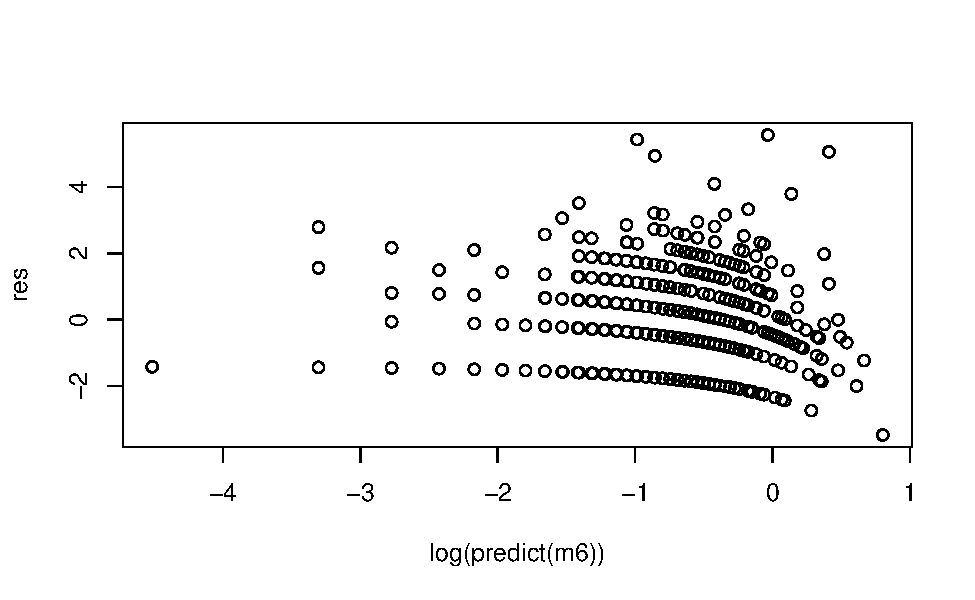
\includegraphics{03-poisson_files/figure-latex/unnamed-chunk-23-1.pdf}

Kontrollime seda ka histogrammiga:

\begin{Shaded}
\begin{Highlighting}[]
\FunctionTok{hist}\NormalTok{(res)}
\end{Highlighting}
\end{Shaded}

\includegraphics{03-poisson_files/figure-latex/unnamed-chunk-24-1.pdf}

Ka siit nähtub, et jäägid ei ole tõesti päris normaalselt jaotunud.

Lõppkokkuvõtteks tuleb tõdeda, et meie mudel ei ole päris ideaalne - ei sobitu kõige paremini andmetega ning ka jääkide struktuur jätab soovida. Põhjus võib olla näiteks selles, et mõni oluline sõltumatu tunnus on mudelist puudu või ka asjaolu, et sõltuva tunnuse jaotus ei vastanud väga hästi Poissoni jaotusele.

  \bibliography{book.bib,packages.bib}

\end{document}
